\documentclass[11pt,oneside]{book}
\usepackage{fontspec}
\usepackage{xeCJK}
\setmainfont{Latin Modern Roman}
\setCJKmainfont[ItalicFont={Noto Serif CJK TC},BoldItalicFont={Noto Serif CJK TC Bold}]{Noto Serif CJK TC}
\setCJKsansfont{Noto Sans CJK TC}
\setCJKmonofont{Noto Sans Mono CJK TC}
\newfontfamily\proseunicodefont{DejaVu Serif}
\usepackage[margin=1in]{geometry}
\usepackage{microtype}
\usepackage{amsmath,amssymb,amsthm,mathtools,bm}
\usepackage{graphicx}
\usepackage{adjustbox}
\usepackage{xcolor}
\usepackage{booktabs}
\usepackage{array}
\usepackage{longtable}
\usepackage{enumitem}
\usepackage{float}
\usepackage{caption}
\usepackage{hyperref}
\usepackage{fancyhdr}
\usepackage{tikz}
\usetikzlibrary{arrows.meta,positioning,calc,decorations.pathmorphing}

\hypersetup{
  colorlinks=true,
  linkcolor=blue!50!black,
  urlcolor=blue!50!black,
  citecolor=blue!50!black
}

\setlength{\parskip}{0.5em}
\setlength{\parindent}{0pt}
\setlist[itemize]{topsep=0.25em,itemsep=0.2em}
\setlist[enumerate]{topsep=0.25em,itemsep=0.2em}
\setlength{\headheight}{40pt}
\numberwithin{equation}{chapter}

\newtheorem{theorem}{定理}[chapter]
\newtheorem{proposition}[theorem]{命題}
\newtheorem{lemma}[theorem]{引理}
\newtheorem{corollary}[theorem]{推論}
\theoremstyle{definition}
\newtheorem{definition}[theorem]{定義}
\newtheorem{example}[theorem]{例}
\theoremstyle{remark}
\newtheorem{remark}[theorem]{註}

\providecommand{\ket}[1]{\left\lvert#1\right\rangle}
\providecommand{\bra}[1]{\left\langle#1\right\rvert}
\providecommand{\braket}[2]{\left\langle#1\,\middle|\,#2\right\rangle}
\providecommand{\expect}[1]{\left\langle#1\right\rangle}
\newcommand{\lectureoverview}[1]{\paragraph{概述。} #1}

\makeatletter
\newcommand{\course@headerfont}{\normalfont\small\itshape}
\newcommand{\course@pagefont}{\normalfont\small}
\newcommand{\course@headerraise}{14pt}
\newlength{\course@headerboxheight}
\setlength{\course@headerboxheight}{\dimexpr\headheight-\course@headerraise-9pt\relax}
\newcommand{\course@leftheadbox}[1]{%
  \raisebox{\course@headerraise}{%
    \parbox[t][\course@headerboxheight][t]{0.82\textwidth}{%
      \raggedright\course@headerfont\strut\MakeUppercase{#1}\strut%
    }%
  }%
}
\newcommand{\course@rightheadbox}[1]{%
  \raisebox{\course@headerraise}{%
    \parbox[t][\course@headerboxheight][t]{0.82\textwidth}{%
      \raggedleft\course@headerfont\strut\MakeUppercase{#1}\strut%
    }%
  }%
}
\renewcommand{\chaptermark}[1]{\markboth{\MakeUppercase{\chaptername\ \thechapter.\ #1}}{}}
\renewcommand{\sectionmark}[1]{\markright{\MakeUppercase{\thesection\hspace{0.4em}#1}}}
\fancyhf{}
\fancyhead[L]{\course@leftheadbox{\leftmark}}
\fancyhead[R]{\course@pagefont\thepage}
\renewcommand{\headrulewidth}{0.5pt}
\pagestyle{fancy}
\fancypagestyle{plain}{%
  \fancyhf{}
  \fancyhead[L]{\course@leftheadbox{\leftmark}}
  \fancyhead[R]{\course@pagefont\thepage}
  \renewcommand{\headrulewidth}{0.5pt}
}
\makeatother

% Video2Book editorial provenance macros
\newenvironment{classroomqa}{%
  \par\medskip\noindent\begin{minipage}{\linewidth}\small\hrule\medskip
}{%
  \medskip\hrule\end{minipage}\par\medskip
}
\newcommand{\audiencequestion}[1]{\noindent\textbf{聽眾提問。} #1\par\smallskip}
\newcommand{\lecturerresponse}[1]{\noindent\textbf{回答。} #1\par}
\newcommand{\lecturetimestamp}[1]{\footnote{講課時間： #1.}}
\newcommand{\lectureframe}[1]{\par\smallskip{\centering\footnotesize\itshape 講課畫面： #1.\par}}
\newcommand{\editorialnote}[1]{\footnote{編者說明： #1}}

\renewcommand{\contentsname}{目錄}
\renewcommand{\chaptername}{章}
\renewcommand{\figurename}{圖}
\renewcommand{\tablename}{表}
\renewcommand{\proofname}{證明}
\renewcommand{\bibname}{參考文獻}
\emergencystretch=2em
\pdfstringdefDisableCommands{\def\proseunicodefont{}}

\geometry{paperwidth=177.6mm,paperheight=252mm,left=16mm,right=16mm,
 top=18mm,bottom=18mm,includeheadfoot,headheight=28pt,headsep=7mm,footskip=9mm}
\usepackage{scrextend}
\changefontsizes[17pt]{12pt}
\raggedbottom
\renewenvironment{classroomqa}{\par\medskip\begingroup}{\par\endgroup\medskip}
\fancyhf{}
\setlength{\headwidth}{\textwidth}
\fancyhead[L]{\parbox{\textwidth}{\raggedright\fontsize{9}{11}\selectfont\nouppercase{\leftmark}}}
\fancyfoot[C]{\small\thepage}
\renewcommand{\headrulewidth}{0.3pt}
\fancypagestyle{plain}{\fancyhf{}\fancyfoot[C]{\small\thepage}\renewcommand{\headrulewidth}{0pt}}

\graphicspath{{../../../generated_course_notes/supplementary/advanced_quantum_mechanics/2013_fall/figures/}{../../../generated_course_notes/supplementary/advanced_quantum_mechanics/2013_fall/assets/}}
\begin{document}
\frontmatter
\hypersetup{pageanchor=false}
\begin{titlepage}
\hyphenpenalty=10000\exhyphenpenalty=10000
\thispagestyle{empty}
\begin{tikzpicture}[remember picture,overlay]
  \node[anchor=center,inner sep=0] at (current page.center) {%
    \includegraphics[height=\paperheight,keepaspectratio]{../../../generated_course_notes/supplementary/advanced_quantum_mechanics/2013_fall/assets/cover-art.png}%
  };
  \node[
    anchor=north west,
    align=left,
    text width=0.78\paperwidth,
    fill=white,
    fill opacity=0.9,
    rounded corners=8pt,
    inner xsep=10pt,
    inner ysep=8pt
  ] at ([xshift=0.08\paperwidth,yshift=-0.06\paperheight]current page.north west) {%
    {\fontsize{30}{33}\selectfont\bfseries\color{black!88} 高等量子力學\\[0.85em]}
    {\large\color{black!72} 繁體中文版 / 2013年秋季}
  };
  \node[
    anchor=south west,
    align=left,
    text width=0.68\paperwidth,
    fill=white,
    fill opacity=0.82,
    text opacity=1,
    rounded corners=6pt,
    inner sep=12pt
  ] at ([xshift=0.08\paperwidth,yshift=0.08\paperheight]current page.south west) {%
    {\normalsize\color{black!78} 原講授：Leonard Susskind\\[0.35em]}
    {\small\color{black!72} 講義輔助版本：\href{https://lazying.art}{LazyingArt LLC} / \href{https://github.com/lachlanchen/Video2Book}{Video2Book}}
  };
\end{tikzpicture}
\mbox{}
\end{titlepage}
\hypersetup{pageanchor=true}

\clearpage
\chapter*{關於本講義}
這些獨立編輯的配套講義依據 Leonard Susskind 的講課內容編寫。講義根據機器轉錄稿、字幕和部分黑板畫面重建，並對照可取得的來源資料核查。這些講義並非 Susskind 教授的原稿，也未經他審閱或認可。

本版由 \href{https://lazying.art}{LazyingArt LLC} 使用開源的 \href{https://github.com/lachlanchen/Video2Book}{Video2Book} 工作流程製作。機器轉錄稿另行提供，可能含有辨識錯誤。編輯上的釐清與實質性重建均以腳註標示。
\clearpage
\tableofcontents
\mainmatter
\chapter{態向量、么正演化與平移對稱性}
\providecommand{\ket}[1]{\left\lvert#1\right\rangle}
\providecommand{\bra}[1]{\left\langle#1\right\rvert}

隔了兩個學季，快速回顧量子力學很有幫助，但不能占滿整個學季。接下來要探討的是量子力學最初發展時所要處理的問題：原子、電子及相關粒子，以及光子。

先談原子。電子是原子的組成部分，為什麼要先講原子，再講電子？一開始只需要足以寫出氫原子基本方程的電子力學。之後再深入研究類電子粒子即可。在這些應用中，對稱性會一再派上用場：對稱性在量子力學中如何表示，以及它對系統有什麼意義。

\section{態、可觀測量與正交性}

在經典力學中，態以相空間中的一個點表示；在量子力學中，則以複向量空間中的一個向量表示。這是抽象向量，不是普通三維空間中的箭頭。態向量可以相加，也可以乘以複數；容納這些向量的空間不必是任何特定的有限維空間。

狄拉克記號將態向量寫成右矢，
\begin{equation}
\ket{\psi},
\end{equation}
並為它配上左矢，
\begin{equation}
\bra{\psi}.
\end{equation}
左矢與右矢透過厄米共軛相互關聯。將左矢與右矢結合可得內積，
\begin{equation}
\langle\phi|\psi\rangle,
\end{equation}
其值一般是複數。

可觀測量是可以測量的物理量，例如位置、動量、能量，或其他可測量的量。在量子力學中，可觀測量以線性厄米算符\(A\)表示，
\begin{equation}
A^\dagger=A.
\end{equation}
厄米性是算符對應於實數性的性質。尤其是，厄米算符的本徵值皆為實數。

\(A\)的本徵向量滿足
\begin{equation}
A\ket{\alpha}=\alpha\ket{\alpha}.
\end{equation}
測量\(A\)可能得到的結果，就是可能的本徵值。例如，若某個可觀測量只能得到\(1\)、\(3\)或\(7\)，這些數就是它的本徵值。它的本徵向量對應於測量結果確定而非統計分布的態。在態\(\ket{\alpha}\)中，測量\(A\)必定得到\(\alpha\)。

內積表達了態之間一種重要的邏輯關係。假設有一種測量，能確定地區分\(\ket{\phi}\)與\(\ket{\psi}\)，那麼這兩個態便互相正交：
\begin{equation}
\langle\phi|\psi\rangle=0.
\end{equation}
正交表示這些態在物理上可以毫無歧義地區分。對於歸一化的態，
\begin{equation}
\langle\psi|\psi\rangle=1.
\end{equation}

\section{位置表象中的粒子}

先考慮一個在直線上運動的粒子。位置\(x\)是可觀測量。對每個可能的位置\(x_0\)，都有一個態\(\ket{x_0}\)，在此態中測量位置必定得到\(x_0\)。

與不同位置相對應的態可以區分，因此彼此正交：
\begin{equation}
x\neq x'
\quad\Longrightarrow\quad
\langle x'|x\rangle=0.
\end{equation}
對任意態\(\ket{\psi}\)，它與位置態的內積定義了波函數：
\begin{equation}
\psi(x)=\langle x|\psi\rangle.
\end{equation}
這就是態向量的位置表象。

波函數本身不是機率。它可以是正數、負數、虛數，或一般的複數。位置機率密度為
\begin{equation}
P(x)=\psi^*(x)\psi(x)=|\psi(x)|^2.
\end{equation}
這個乘積非負，符合機率密度的要求。對歸一化波函數而言，
\begin{equation}
\int_{-\infty}^{\infty}dx\,|\psi(x)|^2=1.
\end{equation}

在位置表象中，位置算符以乘法作用：
\begin{equation}
(\hat x\psi)(x)=x\psi(x).
\end{equation}
它的本徵函數是集中於單一點的理想化函數，形式上以狄拉克 {\proseunicodefont δ} 函數描述，也就是以位置本徵值為中心的極窄尖峰。本次回顧不需要用到它們精確的分佈定義。

在三維空間中，位置有三個分量：\(x\)、\(y\)和\(z\)；位置態則表示三維空間中的一點。只要兩點至少有一個座標不同，對應的態便互相正交。以下通常仍採用一維記號，並假定讀者理解相應的三維推廣。

\section{動量與定動量態}

位置的每個分量都有相對應的動量分量。在位置表象中，沿\(x\)軸的動量算符為
\begin{equation}
\hat p_x=-i\hbar\frac{d}{dx}.
\end{equation}
因此，抽象的厄米算符也可以具體地視為作用於波函數的運算。

具有定動量\(p_0\)的態滿足本徵值方程
\begin{equation}
\hat p_x\psi_{p_0}(x)=p_0\psi_{p_0}(x).
\end{equation}
代入\(\hat p_x\)的微分形式可得
\begin{equation}
-i\hbar\frac{d\psi_{p_0}(x)}{dx}
=p_0\psi_{p_0}(x).
\end{equation}
波函數的導數與波函數本身成正比，因此解具有指數形式：
\begin{equation}
\psi_{p_0}(x)\propto
\exp\left(\frac{ip_0x}{\hbar}\right).
\end{equation}

\begin{classroomqa}
\lecturetimestamp{00:24:26}
\audiencequestion{這個微分方程對所有波函數都成立嗎？}
\lecturerresponse{不成立。這是定動量態的本徵值方程。大多數波函數不滿足這個方程；它選出的是動量本徵函數。}
\end{classroomqa}

位置本徵態與動量本徵態截然不同。位置本徵函數集中在一點；動量本徵函數則滿足
\begin{equation}
\left|\exp\left(\frac{ip_0x}{\hbar}\right)\right|^2=1.
\end{equation}
因此其模在整條直線上皆為常數。在這種理想化的意義下，定動量代表位置完全不確定；定位置也同樣代表動量完全不確定。這是位置--動量不確定關係的極端情形。

\begin{classroomqa}
\lecturetimestamp{00:26:36}
\audiencequestion{若已知動量為\(p_0\)，為什麼仍然有機率分布？}
\lecturerresponse{這裡顯示的量涉及位置測量，而非再次測量動量。位置和動量是不同的可觀測量。對理想化的動量本徵態而言，位置振幅的模在整條直線上皆為常數。動量振幅屬於動量表象，並透過傅立葉變換與位置波函數相互關聯。}
\end{classroomqa}

\begin{classroomqa}
\lecturetimestamp{00:28:02}
\audiencequestion{波函數若是狄拉克 {\proseunicodefont δ} 函數，位置機率會是什麼樣子？}
\lecturerresponse{機率集中在指定位置。這個理想化的尖峰表示位置確定。}
\end{classroomqa}

\editorialnote{精確位置態與定動量態都是廣義態。狄拉克 {\proseunicodefont δ} 函數和平面波都不是定義在整條直線上的普通平方可積、歸一化波函數；而 {\proseunicodefont δ} 函數的平方也不是普通的分佈。前述說法描述的是它們理想化的局域性與常數模。}

形式上，可以把波函數視為一個向量，而\(x\)的每個取值都對應一個分量。不過，它與普通的有限列向量不同，具有連續無窮多個分量。

\begin{classroomqa}
\lecturetimestamp{00:28:53}
\audiencequestion{態向量可以用列向量表示嗎？}
\lecturerresponse{可以，但位置波函數很難寫成普通的列向量，因為\(x\)可以連續取值。形式上可以將它視為連續列向量，並將相應的左矢視為連續行向量。}
\end{classroomqa}

\section{時間演化與么正性}

態如何隨時間改變？時間演化是態空間上的變換。令\(U(t)\)表示經過時間\(t\)的演化，則
\begin{equation}
U(t)\ket{\psi(t_1)}=\ket{\psi(t_1+t)}.
\end{equation}
特別是，
\begin{equation}
\ket{\psi(t)}=U(t)\ket{\psi(0)},
\qquad
U(0)=\mathbf 1.
\end{equation}

對\(U(t)\)的要求源自資訊守恆。若兩個初態可以區分，時間演化就不能抹去這項區別；正交態演化後必須仍然正交。更一般地，任意兩個態之間的內積都保持不變：
\begin{equation}
\langle U(t)\phi|U(t)\psi\rangle
=\langle\phi|\psi\rangle.
\end{equation}
由於
\begin{equation}
\langle U(t)\phi|U(t)\psi\rangle
=\langle\phi|U^\dagger(t)U(t)|\psi\rangle,
\end{equation}
要使所有內積都保持不變，就必須滿足
\begin{equation}
U^\dagger(t)U(t)=\mathbf 1.
\end{equation}
滿足此方程的算符稱為么正算符。

\begin{classroomqa}
\lecturetimestamp{00:36:36}
\audiencequestion{保持所有內積是否比只保持正交性更強？}
\lecturerresponse{對於這裡討論的線性態變換，保持正交性會導致內積也保持不變。熟悉的類比是普通旋轉：旋轉會保持正交性與點積。}
\end{classroomqa}

\editorialnote{嚴格來說，單獨保持正交性仍容許整體乘上一個非零比例因子。物理時間演化本來就必須保持歸一化；這項要求排除了該自由度，因而使內積保持不變。}

么正算符不可與厄米可觀測量混為一談。位置與動量是厄米算符，但一般不是么正算符。么正算符的本徵值是相位，也就是形如\(e^{i\theta}\)、位於單位圓上的數。

\begin{classroomqa}
\lecturetimestamp{00:38:12}
\audiencequestion{非么正變換有哪些例子？}
\lecturerresponse{位置算符與動量算符就是例子：它們是厄米可觀測量，但不是么正算符。么正算符的本徵值模長為一，因此其本徵值是相位。}
\end{classroomqa}

\section{哈密頓量與Schr\"odinger方程}

假設時間演化是連續的。那麼在極短時間間隔\(\epsilon\)內，演化算符必須接近恆等算符：
\begin{equation}
U(\epsilon)=\mathbf 1+\epsilon G+\mathcal O(\epsilon^2).
\end{equation}
利用么正性可得
\begin{align}
U^\dagger(\epsilon)U(\epsilon)
&=
\left(\mathbf 1+\epsilon G^\dagger\right)
\left(\mathbf 1+\epsilon G\right)
+\mathcal O(\epsilon^2)
\\
&=
\mathbf 1+\epsilon(G^\dagger+G)
+\mathcal O(\epsilon^2).
\end{align}
保留一階項後，
\begin{equation}
G^\dagger=-G.
\end{equation}
因此\(G\)是反厄米算符。它可以寫成
\begin{equation}
G=-\frac{i}{\hbar}H,
\end{equation}
其中\(H\)是厄米算符：
\begin{equation}
H^\dagger=H.
\end{equation}
因此，無窮小時間演化算符為
\begin{equation}
U(\epsilon)
=
\mathbf 1-\frac{i\epsilon}{\hbar}H
+\mathcal O(\epsilon^2).
\end{equation}
厄米算符\(H\)就是哈密頓量。

\begin{classroomqa}
\lecturetimestamp{00:45:48}
\audiencequestion{為什麼可以忽略\(\epsilon^2\)項？}
\lecturerresponse{此處的計算一致地只保留\(\epsilon\)的一階項。若要作二階計算，就必須納入所有二階項，包括正比於\(-\epsilon^2H^2/(2\hbar^2)\)的項。近似來自截斷\(U(\epsilon)\)的表示式，而非\(H\)的厄米性。}
\end{classroomqa}

有限時間間隔可以拆成許多小間隔。將\(t\)分成\(N\)個步驟，每一步長度為\(t/N\)。重複施行無窮小變換便得到
\begin{equation}
U(t)
=
\lim_{N\to\infty}
\left(
\mathbf 1-\frac{itH}{N\hbar}
\right)^N
=
\exp\left(-\frac{iHt}{\hbar}\right).
\end{equation}
指數形式就是無窮小變換對應的有限變換。

現在將態從\(t\)演化至\(t+\epsilon\)：
\begin{align}
\ket{\psi(t+\epsilon)}
&=
U(\epsilon)\ket{\psi(t)}
\\
&=
\left(
\mathbf 1-\frac{i\epsilon}{\hbar}H
\right)\ket{\psi(t)}
+\mathcal O(\epsilon^2).
\end{align}
減去\(\ket{\psi(t)}\)，再除以\(\epsilon\)並取極限，可得
\begin{equation}
\frac{d}{dt}\ket{\psi(t)}
=
-\frac{i}{\hbar}H\ket{\psi(t)}.
\end{equation}
等價地，
\begin{equation}
i\hbar\frac{d}{dt}\ket{\psi(t)}
=
H\ket{\psi(t)}.
\end{equation}
這就是含時Schr\"odinger方程。在位置表象中，它成為
\begin{equation}
i\hbar\frac{\partial}{\partial t}\psi(x,t)
=
H\psi(x,t),
\end{equation}
其中\(H\)作為算符作用於波函數。

定態Schr\"odinger方程是哈密頓量的本徵值方程：
\begin{equation}
H\ket{E}=E\ket{E}.
\end{equation}
本徵值\(E\)是測量能量可能得到的值，也就是能階。因此，同一個哈密頓量既決定允許的能量，也決定態如何演化。

若初態是能量本徵態，其演化為
\begin{equation}
\ket{E;t}
=
\exp\left(-\frac{iEt}{\hbar}\right)\ket{E}.
\end{equation}
它仍是同一個能量本徵向量，只多了一個相位。\footnote{負號由前文推導\(U(t)=\exp(-iHt/\hbar)\)所固定。稍後以口語描述此相位時，符號相反，與該推導不一致。}

\begin{classroomqa}
\lecturetimestamp{01:01:05}
\audiencequestion{能量本徵向量依含時Schr\"odinger方程如何演化？}
\lecturerresponse{保留右矢。由於\(H\ket{E}=E\ket{E}\)，時間演化會將能量本徵向量乘上一個由其能量決定的相位：\(\exp(-iEt/\hbar)\)。}
\end{classroomqa}

\section{什麼才算對稱性？}

時間演化是態空間上的一種么正變換。對稱變換則是另一類重要的變換。

旋轉對稱性在原子物理中至關重要。在氫原子中，電子在中心庫侖勢中運動。旋轉座標系不會改變方程；將原子實際旋轉後，它仍是由相同方程支配的氫原子。態可能隨旋轉而改變，但動力學定律不變。

平移是另一個例子。在空曠空間中的孤立系統，若將系統各部分都位移相同距離，其行為應該相同。這個條件很重要。若附近有一座爐子，而只將系統移得更靠近爐子，系統的行為可能改變；爐子會破壞平移對稱性。若系統與爐子一起平移，它們原有的相對關係便會恢復。

並非任何操作都是對稱性。將岩鹽晶體壓縮至原來的一半，通常會改變其行為。擠壓是一種定義明確的變換，但一般不具對稱性。

因此，對稱性是作用於態、並保持動力學形式不變的操作。以\(V\)表示此操作。它必須保持態的可區分性：兩個正交態經變換後仍須正交。相應地，
\begin{equation}
V^\dagger V=\mathbf 1,
\end{equation}
因此\(V\)是么正的。

\section{對稱性與時間演化對易}

假設初態\(\ket{\psi_1}\)演化成\(\ket{\psi_2}\)：
\begin{equation}
\ket{\psi_2}=U(t)\ket{\psi_1}.
\end{equation}
將候選對稱操作\(V\)作用於這兩個態：
\begin{equation}
\ket{\psi_1'}=V\ket{\psi_1},
\qquad
\ket{\psi_2'}=V\ket{\psi_2}.
\end{equation}
若\(V\)是動力學的對稱性，變換後的初態必須演化成變換後的末態：
\begin{equation}
\ket{\psi_2'}=U(t)\ket{\psi_1'}.
\end{equation}
代入定義可得
\begin{equation}
VU(t)\ket{\psi_1}
=
U(t)V\ket{\psi_1}.
\end{equation}
此式必須對所有初態成立。因此
\begin{equation}
VU(t)=U(t)V.
\end{equation}

這兩條等價路徑可以用交換圖表示。\footnote{此圖重現了01：10：30至01：16：34之間所建立的兩條路徑論證。}
\begin{figure}
\centering
\begin{tikzpicture}[>=Stealth]
\node (a) at (0,0) {$\ket{\psi_1}$};
\node (b) at (4.2,0) {$\ket{\psi_2}=U(t)\ket{\psi_1}$};
\node (c) at (0,-2.0) {$V\ket{\psi_1}$};
\node (d) at (4.2,-2.0) {$V\ket{\psi_2}=U(t)V\ket{\psi_1}$};

\draw[->] (a) -- node[above] {$U(t)$} (b);
\draw[->] (c) -- node[below] {$U(t)$} (d);
\draw[->] (a) -- node[left] {$V$} (c);
\draw[->] (b) -- node[right] {$V$} (d);
\end{tikzpicture}
\caption{無論先施行對稱操作或先作時間演化，得到的末態都相同。}
\end{figure}

\begin{classroomqa}
\lecturetimestamp{01:16:38}
\audiencequestion{對稱性是否必須在所有時間都與時間演化對易？}
\lecturerresponse{是。動力學的對稱性必須與完整的時間演化滿足對易條件。}
\end{classroomqa}

\begin{classroomqa}
\lecturetimestamp{01:17:13}
\audiencequestion{這是否表示可以先旋轉再等待，或先等待再旋轉？}
\lecturerresponse{正是如此。若旋轉是對稱性，無論採用哪個順序，得到的變換後末態都相同。}
\end{classroomqa}

對於一段很短的時間間隔，
\begin{equation}
U(\epsilon)
=
\mathbf 1-\frac{i\epsilon}{\hbar}H
+\mathcal O(\epsilon^2).
\end{equation}
對易條件變成
\begin{equation}
V\left(
\mathbf 1-\frac{i\epsilon}{\hbar}H
\right)
=
\left(
\mathbf 1-\frac{i\epsilon}{\hbar}H
\right)V
+\mathcal O(\epsilon^2).
\end{equation}
恆等算符項相消後，剩下
\begin{equation}
VH=HV,
\end{equation}
亦即
\begin{equation}
[V,H]=0.
\end{equation}
因此，么正操作若且唯若與哈密頓量對易，便是動力學的對稱性。

\begin{classroomqa}
\lecturetimestamp{01:19:29}
\audiencequestion{為什麼要求對稱算符\(V\)必須是么正的？}
\lecturerresponse{對稱性必須保留態之間的邏輯區別。它不應將兩個互斥且正交的態變成無法區分的態。要保留這些關係，就必須是么正變換。}
\end{classroomqa}

不顯含時間且與\(H\)對易的算符是守恆量。這使對稱性與守恆律相連。在經典力學中，這種關係由諾特定理表述。在此處的量子力學形式中，關鍵判準是算符與哈密頓量的對易子。

\section{離散與連續對稱性}

對稱性可以是離散的，也可以是連續的。鏡射是離散對稱操作：它交換左右，但兩者之間不存在一連串無窮小鏡射。交換兩個全同粒子也是離散操作。翻轉一個沒有標記的雙面物體，也是同類例子。

旋轉是連續的。\(90^\circ\)的旋轉可以由許多繞同一軸的小角度旋轉組成。空間平移也基於相同理由而連續：有限位移可以分解成許多微小位移。

能夠分解成小變換，使連續對稱性具有一種特殊形式。在恆等變換附近，可寫成
\begin{equation}
V(\epsilon)
=
\mathbf 1-i\epsilon G+\mathcal O(\epsilon^2),
\end{equation}
其中\(\epsilon\)是描述該變換的參數。么正性要求
\begin{equation}
G^\dagger=G.
\end{equation}
厄米算符\(G\)稱為此對稱性的生成元。

若此變換是對稱性，則
\begin{equation}
[H,V(\epsilon)]=0.
\end{equation}
展開至一階可得
\begin{equation}
[H,G]=0.
\end{equation}
因此，連續對稱性由與哈密頓量對易的厄米算符生成。這些生成元就是守恆量。

``生成''在此有明確的意思：反覆施行無窮小變換，就能構成有限變換；這和以許多短時間步構成有限時間演化相同。

\section{平移對稱性與動量}

考慮將波函數主動向右平移距離\(\epsilon\)。若原波函數在\(x_0\)處有峰值，平移後的波函數便應在\(x_0+\epsilon\)處有峰值。因此，平移後波函數在座標\(x\)處的值，等於原波函數在\(x-\epsilon\)處的值：
\begin{equation}
(T(\epsilon)\psi)(x)=\psi(x-\epsilon).
\end{equation}
對於小位移，
\begin{equation}
\psi(x-\epsilon)
=
\psi(x)-\epsilon\frac{d\psi(x)}{dx}
+\mathcal O(\epsilon^2).
\end{equation}
因此
\begin{equation}
T(\epsilon)
=
\mathbf 1-\epsilon\frac{d}{dx}
+\mathcal O(\epsilon^2).
\end{equation}
利用
\begin{equation}
\hat p_x=-i\hbar\frac{d}{dx},
\qquad
\frac{d}{dx}=\frac{i}{\hbar}\hat p_x,
\end{equation}
無窮小平移便成為
\begin{equation}
T(\epsilon)
=
\mathbf 1-\frac{i\epsilon}{\hbar}\hat p_x
+\mathcal O(\epsilon^2).
\end{equation}
相應的有限平移為
\begin{equation}
T(\epsilon)
=
\exp\left(-\frac{i\epsilon}{\hbar}\hat p_x\right).
\end{equation}
採用約定\(V(\epsilon)=\mathbf 1-i\epsilon G+\cdots\)時，有量綱的平移參數給出
\begin{equation}
G_{\mathrm{trans}}=\frac{\hat p_x}{\hbar}.
\end{equation}
換言之，若在指數中明確寫出\(\hbar\)因子，動量便稱為空間平移的生成元。

\begin{classroomqa}
\lecturetimestamp{01:34:08}
\audiencequestion{平移推導是不是漏了一個負號？}
\lecturerresponse{問題在於如何指定平移後波函數的方向。主動向右平移應以\(\psi(x-\epsilon)\)表示，而非\(\psi(x+\epsilon)\)。修正後可得\(T(\epsilon)=\mathbf 1-i\epsilon\hat p_x/\hbar+\cdots\)。}
\end{classroomqa}

動量是否守恆取決於哈密頓量。對於在一維運動的自由粒子，
\begin{equation}
H=\frac{\hat p_x^2}{2m}.
\end{equation}
由於任何算符都與自身的任意函數對易，
\begin{equation}
[H,\hat p_x]=0.
\end{equation}
因此自由粒子的哈密頓量具有平移不變性，而\(\hat p_x\)守恆。從物理上來說，無論初始位置在哪裡，粒子的行為都相同。平移初始條件只會使整個運動相應平移。

在三維中，
\begin{equation}
H
=
\frac{\hat p_x^2+\hat p_y^2+\hat p_z^2}{2m}.
\end{equation}
每個動量分量都與\(H\)對易：
\begin{equation}
[H,\hat p_x]=[H,\hat p_y]=[H,\hat p_z]=0.
\end{equation}
每個空間方向各有一種平移對稱性。動量既是守恆量，也是這些平移所對應的生成元。

接下來討論旋轉對稱性。旋轉較為複雜，因為繞不同軸旋轉通常不對易：先繞\(x\)軸旋轉再繞\(y\)軸旋轉，與反過來的順序並不相同。這會導致對稱性生成元不對易，並引出旋轉的群論結構。

\chapter{對稱性、簡併與角動量階梯}
\providecommand{\ket}[1]{\left\lvert#1\right\rangle}

\section{對稱性與簡併能階}

對稱性是一種不改變系統物理描述的操作。它不會改變哈密頓量、Schr\"odinger方程或可能的能量。若以么正算符\(S\)表示此操作，不變性便意味著
\begin{equation}
S H S^\dagger=H,
\end{equation}
或等價地
\begin{equation}
[S,H]=0.
\end{equation}

平移就是一個例子。將原子從一處移到另一處，原子的能量不會改變。這對所有原子態都成立，不只對基態如此。旋轉是另一個例子，也是本節的主要主題。

交換兩個全同粒子也是一種對稱性。把兩個電子稱為電子一和電子二，或稱為 Harry 和 Fred，都不會使它們變得不同。交換標記不會改變原子的性質。

晶體還有一種額外的平移對稱性。將整個晶體在空間中平移，是一般的平移。然而，對無限晶體而言，平移一個晶格間距後，物理排列也會保持不變。等價地說，將每個格點的標號都平移一格，就能重新標記格點。有限晶體的邊界會使這個說法不再嚴格成立；但在很長的晶體中，遠離兩端之處仍可視為具有這項近似對稱性。

空間的均勻性---也就是每個位置都和其他位置一樣---就是平移對稱性。空間的各向同性---也就是每個方向都和其他方向一樣---就是旋轉對稱性。

簡併與對稱性有關，但兩者並不相同。若不只一個態具有完全相同的能量，這個能階便是簡併的。對於具有離散譜的一般哈密頓量，兩個互不相關的能階恰好完全相等，會是驚人的巧合。即使兩者相差不到\(10^{15}\)，仍不代表完全相等。精確簡併通常暗示著對稱性。

對稱性有時會導致簡併，但並非總是如此。第一個例子會說明對稱性為何可能導致簡併，也會說明為何單靠一種對稱性有時還不夠。

\section{圓上的粒子}

考慮一顆被限制在圓形軌道上運動的珠子。它的位置可以用笛卡兒座標\(x\)和\(y\)描述，但只用一個角座標就足夠：
\begin{equation}
\psi=\psi(\theta).
\end{equation}
圓上的位置機率密度為\(\psi^*(\theta)\psi(\theta)\)。

逆時針主動旋轉一個小角度\(\epsilon\)後，波函數變為
\begin{equation}
\psi(\theta)\longrightarrow\psi(\theta-\epsilon).
\end{equation}
因此
\begin{align}
\delta\psi(\theta)
&=\psi(\theta-\epsilon)-\psi(\theta)\\
&=-\epsilon\frac{d\psi}{d\theta}
+\mathcal O(\epsilon^2).
\end{align}

算符
\begin{equation}
L_z=-i\hbar\frac{d}{d\theta}
\end{equation}
作用在週期波函數上時是厄米算符。它是
\begin{equation}
p_x=-i\hbar\frac{d}{dx}.
\end{equation}
在角座標中的類比。因子\(i\)對厄米性至關重要。以\(L_z\)表示，
\begin{equation}
\delta\psi
=-\frac{i\epsilon}{\hbar}L_z\psi
+\mathcal O(\epsilon^2),
\end{equation}
所以無窮小旋轉算符為
\begin{equation}
R(\epsilon)
=1-\frac{i\epsilon}{\hbar}L_z
+\mathcal O(\epsilon^2).
\end{equation}
這表示\(L_z\)是繞垂直於圓面的軸旋轉時的生成元。

\begin{classroomqa}
\lecturetimestamp{00:11:19}
\audiencequestion{涉及\(i\)的其中一個因子，符號是否應該相反？}
\lecturerresponse{檢查符號後，就得到上面的關係。按照約定\(\psi(\theta)\to\psi(\theta-\epsilon)\)，變化量是\(-\epsilon\,d\psi/d\theta\)，而這等於\(-i\epsilon L_z\psi/\hbar\)。}
\end{classroomqa}

現在求角動量的本徵態：
\begin{equation}
L_z\psi=M\psi.
\end{equation}
代入微分算符後得到
\begin{equation}
-i\hbar\frac{d\psi}{d\theta}=M\psi,
\end{equation}
其解的形式為
\begin{equation}
\psi(\theta)=C\exp\left(\frac{iM\theta}{\hbar}\right).
\end{equation}

這裡還有一個在無限直線上的運動不會遇到的額外條件。\(\theta=0\)和\(\theta=2\pi\)是同一個點，因此單值的軌道波函數必須滿足
\begin{equation}
\psi(\theta+2\pi)=\psi(\theta).
\end{equation}
對於上面的本徵函數，這表示
\begin{equation}
\exp\left(\frac{2\pi iM}{\hbar}\right)=1.
\end{equation}
因此，
\begin{equation}
M=m\hbar,
\qquad
m\in\mathbb Z.
\end{equation}
圓上的軌道角動量可能值為
\begin{equation}
\ldots,-2\hbar,-\hbar,0,\hbar,2\hbar,\ldots.
\end{equation}

角動量為\(m\hbar\)的態，是否必須與角動量為\(-m\hbar\)的態具有相同能量？正、負\(m\)代表環流方向相反。問題是，單靠旋轉對稱性，是否就能要求這兩種運動具有相同能量？

\begin{classroomqa}
\lecturetimestamp{00:22:51}
\audiencequestion{採用\(\psi(\theta-\epsilon)\)這個形式，是否表示粒子正順時針運動？}
\lecturerresponse{不是。這個約定只決定哪個方向稱為正向旋轉。它定義角位置和角動量的正負號，卻不決定粒子實際運動的方向。}
\end{classroomqa}

垂直於圓面方向的磁場提供了一個反例。它可以使正、負角動量對應的能量朝相反方向移動，因而使兩者的能量分裂。能量位移的正負取決於電荷與方向的約定；此處重要的是能量分裂這件事。

這種磁場仍保有繞垂直軸的旋轉對稱性。因此，它顯示單靠旋轉對稱性並不能要求
\begin{equation}
E(m)=E(-m).
\end{equation}
若沒有能量分裂，\(m=1\)和\(m=-1\)可以形成一對簡併態，\(m=2\)和\(m=-2\)也可以。態\(m=0\)則沒有這種不同的配對態。

\section{\texorpdfstring{\(m,-m\)}{m, -m}對與反射對稱性}

再加入一種離散反射對稱性。令\(\mathcal M\)表示對圓的一條直徑作鏡射：
\begin{equation}
(\mathcal M\psi)(\theta)=\psi(-\theta).
\end{equation}
它會反轉環流方向：
\begin{equation}
\mathcal M\psi_m=\psi_{-m}.
\end{equation}

若反射是對稱操作，則
\begin{equation}
[\mathcal M,H]=0.
\end{equation}
假設
\begin{equation}
H\ket{m}=E_m\ket{m}.
\end{equation}
作用\(\mathcal M\)後得到
\begin{align}
H\mathcal M\ket{m}
&=\mathcal M H\ket{m}\\
&=E_m\mathcal M\ket{m}.
\end{align}
由於\(\mathcal M\ket{m}\)是角動量為\(-m\hbar\)的態，
\begin{equation}
E_{-m}=E_m.
\end{equation}
旋轉對稱性使角動量守恆；反射對稱性則把兩個相反的角動量值聯繫起來。兩者合在一起，便要求這一對態簡併。

\begin{classroomqa}
\lecturetimestamp{00:29:54}
\audiencequestion{既然\(m\)和\(-m\)態具有相同的機率密度，這是否已足以顯示它們的能量相等？}
\lecturerresponse{不。波函數\(e^{im\theta}\)和\(e^{-im\theta}\)本身不同，儘管它們的絕對值平方相同。角動量本徵值方程涉及波函數本身，而不只是\(\psi^*\psi\)。量子力學需要的是振幅，不能只看機率。}
\end{classroomqa}

磁場保有繞其軸的旋轉對稱性，卻破壞了前面所用的反射對稱性。

\begin{classroomqa}
\lecturetimestamp{00:33:05}
\audiencequestion{反射對稱性會使磁場反向嗎？}
\lecturerresponse{會。磁場是軸向量。將指向紙面內的磁場作鏡射，會得到指向紙面外的磁場。等價地說，電流環及其鏡像中的電流方向相反，因此產生方向相反的磁場。}
\end{classroomqa}

旋轉與反射不對易，這點可以直接看出。作用在角動量本徵函數上時，
\begin{align}
\mathcal M L_z\psi_m
&=m\hbar\,\psi_{-m},\\
L_z\mathcal M\psi_m
&=-m\hbar\,\psi_{-m}.
\end{align}
因此
\begin{equation}
[\mathcal M,L_z]\psi_m
=2m\hbar\,\psi_{-m},
\end{equation}
當\(m\neq0\)時，結果不為零。先旋轉再反射，與先反射再旋轉，並非同一個操作。

當兩種變換都是對稱操作時，兩個算符都與\(H\)對易，但兩者彼此不對易。這就是導致簡併的模式。

\begin{classroomqa}
\lecturetimestamp{00:40:28}
\audiencequestion{任意一對不對易的海森堡算符，例如\(x\)和\(p\)，都會產生簡併嗎？}
\lecturerresponse{一般而言不會。這些算符還必須是對稱性，也就是必須與哈密頓量對易。位置和動量通常不會同時守恆。若兩者確實都與\(H\)對易，那麼它們的不對易性就會意味著簡併。}
\end{classroomqa}

\section{對稱性的對易子代數}

假設\(A\)和\(B\)是兩個連續對稱性的厄米生成元：
\begin{equation}
[A,H]=0,
\qquad
[B,H]=0.
\end{equation}
這些方程並未要求\(A\)和\(B\)彼此對易。

對易子\([A,B]\)是反厄米的，因此定義一個厄米算符
\begin{equation}
C=i[A,B].
\end{equation}
此處數值因子和整體正負號並不重要。關鍵是\(C\)也與哈密頓量對易。確實，
\begin{equation}
[AB,H]
=A[B,H]+[A,H]B=0,
\end{equation}
同樣地
\begin{equation}
[BA,H]=0.
\end{equation}
因此
\begin{equation}
[C,H]
=i\bigl([AB,H]-[BA,H]\bigr)=0.
\end{equation}

新的生成元\(C\)可能獨立於\(A\)和\(B\)，也可能只是已知生成元的線性組合。若它是新的，就將它加入列表，再計算更多對易子。這個過程可能無限延續，但通常會在有限個生成元之後閉合：所有後續對易子都是現有生成元的線性組合。這個閉合的系統稱為對易子代數或李代數。

有限的對稱變換構成一個群；它們的無窮小生成元則構成相應的李代數。

簡併之所以重要，是因為它能整理能譜。若兩個態能量相同，一個態就不能藉由發射能量等於兩態能量差的光子而衰變至另一個態。在原子光譜學中，能階的排列方式及其簡併情形決定可能出現的譜線。同樣的道理也適用於激發態強子及其躍遷。

\begin{classroomqa}
\lecturetimestamp{00:49:07}
\audiencequestion{這些對易子本身是對稱群的元素嗎？}
\lecturerresponse{這裡討論的是生成元。生成元及其對易子構成對易子代數，也就是李代數。由生成元構成的有限對稱操作才是群元素。}
\end{classroomqa}

若所有對稱性生成元彼此對易，這種對稱性稱為阿貝爾對稱性。若有些生成元的對易子不為零，則稱為非阿貝爾對稱性。

\begin{classroomqa}
\lecturetimestamp{00:50:25}
\audiencequestion{生成元的根本定義是什麼？}
\lecturerresponse{取一個非常接近恆等變換的么正對稱變換，將它寫成\(1-i\epsilon G/\hbar+\cdots\)。厄米算符\(G\)就是這個變換的生成元。重複相應的無窮小變換，就能構成有限變換。}
\end{classroomqa}

\begin{classroomqa}
\lecturetimestamp{00:52:08}
\audiencequestion{對稱性生成元的代數是什麼意思？}
\lecturerresponse{它是由一組生成元構成的集合；這些生成元可以相加、相減、乘以一般數值，也可以彼此取對易子。在這個代數中，對易子扮演乘法的角色；封閉性表示這些運算不會產生集合以外的生成元。}
\end{classroomqa}

\section{繞不同軸旋轉}

旋轉是非阿貝爾對稱性最重要的例子。先繞\(x\)軸旋轉，再繞\(y\)軸旋轉，一般不等同於以相反順序進行這兩次旋轉。兩種順序之間的差異本身與繞第三軸旋轉有關。

\begin{classroomqa}
\lecturetimestamp{00:54:22}
\audiencequestion{有限旋轉不對易，但無窮小旋轉是否對易？}
\lecturerresponse{兩者的差異出現在兩個小旋轉角的二階項。這就足夠了：提出這兩個小角度因子後，生成元本身的對易子仍不為零。}
\end{classroomqa}

在計算量子對易子之前，先看看對應的經典圖像。考慮一個圓形行星軌道，其角動量垂直於軌道平面。將整個軌道繞\(y\)軸旋轉，會得到另一個能量完全相同的允許軌道。不過，這個軌道的角動量向量現在具有不同的\(x\)分量。

因此，旋轉不變性會產生能量相同、角動量分量不同的組態。在量子力學中，這表現為繞不同軸旋轉的生成元彼此不對易。

\section{笛卡兒座標中的角動量}

先考慮一個在\(xy\)平面內運動、但不受限於圓周的粒子。作微小的逆時針旋轉時，
\begin{equation}
\delta x=-\epsilon y,
\qquad
\delta y=\epsilon x.
\end{equation}
對於主動旋轉後的態，變換後的波函數要在逆旋轉後的座標處取值：
\begin{equation}
\psi_\epsilon(x,y)
=\psi(x+\epsilon y,y-\epsilon x).
\end{equation}
因此，
\begin{align}
\delta\psi
&=\epsilon\left(
y\frac{\partial}{\partial x}
-x\frac{\partial}{\partial y}
\right)\psi
+\mathcal O(\epsilon^2)\\
&=-\frac{i\epsilon}{\hbar}
\left(xp_y-yp_x\right)\psi
+\mathcal O(\epsilon^2).
\end{align}
所以，繞\(z\)軸旋轉的生成元為
\begin{equation}
L_z=xp_y-yp_x.
\end{equation}
這就是熟知的經典向量
\begin{equation}
\mathbf L=\mathbf r\times\mathbf p.
\end{equation}
的\(z\)分量。它不只是力學角動量；在量子力學中，它也是使波函數旋轉的算符。\footnote{採用主動旋轉約定，是為了與先前的變換\(\psi(\theta)\mapsto\psi(\theta-\epsilon)\)以及口頭推導中經過符號確認後得到的結果\(L_z=xp_y-yp_x\)一致。}

對\(x\to y\to z\to x\)作循環置換，就能得到其他分量。\footnote{\(L_x\)和\(L_y\)的公式，是依照講課中明確指定的循環置換\(x\to y\to z\to x\)，由\(L_z=xp_y-yp_x\)推得的。}
\begin{align}
L_x&=yp_z-zp_y,\\
L_y&=zp_x-xp_z,\\
L_z&=xp_y-yp_x.
\end{align}

對於旋轉不變的系統，這些算符都與哈密頓量對易：
\begin{equation}
[H,L_x]=[H,L_y]=[H,L_z]=0.
\end{equation}
在中心力場中運動的粒子是標準例子。這些方程就是角動量守恆的量子形式。

\section{角動量李代數}

正則對易關係為
\begin{align}
[x_i,x_j]&=0,\\
[p_i,p_j]&=0,\\
[x_i,p_j]&=i\hbar\,\delta_{ij}.
\end{align}
座標與不同方向的動量分量彼此對易。因此，例如\(x\)與\(p_y\)對易，而\(x\)與\(p_x\)不對易。

現在計算
\begin{equation}
[L_x,L_y]
=
[yp_z-zp_y,\;zp_x-xp_z].
\end{equation}
大多數項都會消失。僅有兩個非零項：
\begin{align}
[yp_z,zp_x]&=-i\hbar\,yp_x,\\
[zp_y,xp_z]&=i\hbar\,xp_y.
\end{align}
因此
\begin{align}
[L_x,L_y]
&=i\hbar\left(xp_y-yp_x\right)\\
&=i\hbar L_z.
\end{align}
對座標標記作循環置換，可得
\begin{align}
[L_x,L_y]&=i\hbar L_z,\\
[L_y,L_z]&=i\hbar L_x,\\
[L_z,L_x]&=i\hbar L_y.
\end{align}

\begin{classroomqa}
\lecturetimestamp{01:14:50}
\audiencequestion{當對易子產生\(L_z\)時，我們是否仍須證明\(L_z\)不是\(L_x\)和\(L_y\)的線性組合？}
\lecturerresponse{是的。必須證明它們彼此獨立，不能直接假定如此。此處不進一步作直接的代數證明。}
\end{classroomqa}

上面列出的對易關係在\(L_x\)、\(L_y\)和\(L_z\)所張成的空間中閉合：將三者都納入後，後續的對易運算不會產生此空間以外的算符。這就是角動量李代數。再加上
\begin{equation}
[H,L_i]=0,
\qquad i=x,y,z,
\end{equation}
這些關係便包含了能譜的大量資訊，無須直接求解角向Schr\"odinger方程。

量子諧振子也採用類似的代數方法，以產生算符和湮滅算符生成其能譜。在這裡，類似的算符改變的是角動量的\(z\)分量，而不是能量。

選擇\(z\)軸只是選擇一種表象。物理上並沒有理由認為\(z\)比\(x\)或\(y\)更特殊，但選定一個分量可得到方便的基底。令
\begin{equation}
L_z\ket{m}=m\hbar\ket{m}.
\end{equation}
我們要找出\(m\)可能取哪些值，以及不同\(m\)的態之間有何關係。

\begin{classroomqa}
\lecturetimestamp{01:24:02}
\audiencequestion{你將這個構造和諧振子比較時，指的是量子諧振子嗎？上一堂課並沒有講到它。}
\lecturerresponse{是的，比較的對象是量子諧振子。這裡的角動量論證本身完整，不需要先了解諧振子。之後也可以反過來看這個類比：諧振子同樣運用了類似的代數方法。}
\end{classroomqa}

\section{角動量的升降算符}

定義
\begin{equation}
L_+=L_x+iL_y,
\qquad
L_-=L_x-iL_y.
\end{equation}
角動量的對易關係給出
\begin{equation}
[L_z,L_+]=\hbar L_+,
\qquad
[L_z,L_-]=-\hbar L_-.
\end{equation}

將第一個關係式作用在\(L_z\)的本徵態上：
\begin{align}
L_zL_+\ket{m}
&=\left(L_+L_z+[L_z,L_+]\right)\ket{m}\\
&=(m+1)\hbar\,L_+\ket{m}.
\end{align}
除非\(L_+\ket{m}=0\)，否則所得結果是\(L_z\)的另一個本徵態，其本徵值為\((m+1)\hbar\)。同樣地，
\begin{equation}
L_zL_-\ket{m}
=(m-1)\hbar\,L_-\ket{m}.
\end{equation}
因此，\(L_+\)會使\(m\)增加一，而\(L_-\)會使它減少一。

從任一個本徵值出發，代數會產生一個彼此相差整數的序列。這個序列可能無限延伸，也可能因為在上端有
\begin{equation}
L_+\ket{m_{\mathrm{top}}}=0
\end{equation}
以及在下端有
\begin{equation}
L_-\ket{m_{\mathrm{bottom}}}=0
\end{equation}
而終止。

\begin{classroomqa}
\lecturetimestamp{01:35:11}
\audiencequestion{圓的例子不是已經要求角動量必須是整數了嗎？}
\lecturerresponse{那個論證證明，由單值的位置波函數表示的軌道角動量必須取整數值。抽象的角動量代數給出的結果較寬鬆：階梯上可以是整數，也可以是半整數。}
\end{classroomqa}

如果階梯終止，旋轉不變性會把它的兩端聯繫起來。繞垂直於\(z\)的軸旋轉\(180^\circ\)，會使
\begin{equation}
L_z\longrightarrow-L_z.
\end{equation}
因此，譜必須以零為中心對稱：
\begin{equation}
m_{\mathrm{bottom}}=-m_{\mathrm{top}}.
\end{equation}
由於相鄰值相差一，可能的情形有兩種。階梯上的值可以是整數，
\begin{equation}
\ldots,-2,-1,0,1,2,\ldots,
\end{equation}
也可以是半整數，
\begin{equation}
\ldots,-\frac{5}{2},-\frac{3}{2},-\frac{1}{2},
\frac{1}{2},\frac{3}{2},\frac{5}{2},\ldots,
\end{equation}
其端點則位於升算符或降算符作用後結果為零之處。

圓上的單值波函數論證，為軌道角動量選出整數這種可能性，
\begin{equation}
\mathbf L=\mathbf r\times\mathbf p.
\end{equation}
半整數的可能性也符合物理實況，屬於自旋角動量，稍後會另外討論。

最後，若哈密頓量具有旋轉不變性，階梯上的態就具有相同能量。假設
\begin{equation}
H\ket{m}=E\ket{m}.
\end{equation}
由於每個分量\(L_i\)都與\(H\)對易，\(L_+\)和\(L_-\)也會與它對易。因此
\begin{align}
H L_+\ket{m}
&=L_+H\ket{m}\\
&=E L_+\ket{m}.
\end{align}
只要\(L_+\ket{m}\neq0\)，升階後的態就與原態具有相同能量。同樣的計算也會得到
\begin{equation}
H L_-\ket{m}=E L_-\ket{m}.
\end{equation}
因此，升降算符會生成一族\(L_z\)本徵值不同、能量卻完全相同的態。這就是本講一路探討的非對易對稱性與簡併之間的關聯。

\begin{classroomqa}
\lecturetimestamp{01:44:13}
\audiencequestion{這些階梯態是否對應於選擇不同的旋轉軸？}
\lecturerresponse{它們彼此可透過旋轉聯繫。\(L_x\)或\(L_y\)的本徵向量，都是所選\(L_z\)本徵向量的線性組合。旋轉一個態會改變它的角動量分量，但不改變它的能量。}
\end{classroomqa}

選擇\(L_+\)和\(L_-\)很方便，因為這兩個組合能直接呈現階梯結構。這種技巧在量子力學中一再出現：若對易子代數閉合，升算符和降算符往往能整理本徵值譜。

\begin{classroomqa}
\lecturetimestamp{01:46:33}
\audiencequestion{當\(L_+\)作用在最高態上時會怎樣？最高態如何定義？}
\lecturerresponse{作用結果為零，這就是終止階梯頂端的定義。同樣地，\(L_-\)在底端作用時也會得到零。抽象的階梯不一定會終止；不過，對於稍後要討論的原子角動量態，階梯通常會終止。}
\end{classroomqa}

下一步是進一步發展這套角動量結構，並將它應用於原子，包括氫原子。這裡找到的旋轉多重態解釋了部分簡併模式，還有其他結構需要進一步探討。
\chapter{角動量多重態、徑向運動與振子階梯}

\section{波函數的角度依賴}

中心力場中的粒子具有徑向座標和兩個角座標。經典力學中，
\begin{equation}
\mathbf L=\mathbf r\times\mathbf p
\end{equation}
是一個守恆向量。它的方向決定軌道平面，但軌道不一定是圓形。

量子力學中，粒子以
\begin{equation}
\Psi=\Psi(r,\theta,\phi),
\end{equation}
描述；角動量則與此波函數對角度的依賴有關。

在二維中，角動量只有一個分量，也就是繞垂直於平面的軸旋轉的生成元：
\begin{equation}
L_z=-i\hbar\frac{\partial}{\partial\theta}.
\end{equation}
本徵值為\(\hbar\ell\)的本徵函數滿足
\begin{equation}
-i\hbar\frac{\partial}{\partial\theta}\psi(r,\theta)
=\hbar\ell\,\psi(r,\theta).
\end{equation}
在這個方程中，座標\(r\)不受影響。方程的解具有以下形式：
\begin{equation}
\psi(r,\theta)=\chi(r)e^{i\ell\theta}.
\end{equation}
對於普通的單值軌道波函數，當\(\theta\to\theta+2\pi\)後回到同一點，要求\(\ell\)為整數。徑向因子\(\chi(r)\)可能影響能量，但不影響這個角動量本徵值。

三維的對應情形也能將徑向依賴與球面上的函數分離：
\begin{equation}
\Psi(r,\theta,\phi)=R(r)Y_{\ell m}(\theta,\phi).
\end{equation}
函數\(Y_{\ell m}\)稱為球諧函數。此處不需要它們的明確公式。旋轉作用在角度因子上，而徑向函數不變。

\section{有限角動量多重態}

角動量的分量滿足
\begin{equation}
\begin{aligned}
[L_x,L_y]&=i\hbar L_z,\\
[L_y,L_z]&=i\hbar L_x,\\
[L_z,L_x]&=i\hbar L_y.
\end{aligned}
\end{equation}
選取\(L_z\)的本徵態，
\begin{equation}
L_z|\ell,m\rangle=\hbar m\,|\ell,m\rangle,
\end{equation}
並定義
\begin{equation}
L_\pm=L_x\pm iL_y.
\end{equation}
由對易關係
\begin{equation}
[L_z,L_\pm]=\pm\hbar L_\pm
\end{equation}
可得
\begin{align}
L_z\bigl(L_\pm|\ell,m\rangle\bigr)
&=\bigl(L_\pm L_z+[L_z,L_\pm]\bigr)|\ell,m\rangle \\
&=\hbar(m\pm1)L_\pm|\ell,m\rangle.
\end{align}
因此，\(L_+\)會使\(m\)增加一，而\(L_-\)會使它減少一，除非所得向量為零。

有限多重態有一個最高態和一個最低態：
\begin{equation}
L_+|\ell,\ell\rangle=0,
\qquad
L_-|\ell,-\ell\rangle=0.
\end{equation}
\(+z\)與\(-z\)方向可以透過旋轉互相對應，因此有限譜以零為中心對稱。其取值為
\begin{equation}
m=-\ell,-\ell+1,\ldots,\ell-1,\ell,
\end{equation}
態的數目則是
\begin{equation}
2\ell+1.
\end{equation}
相鄰取值相差一，因此端點可以是整數或半整數。普通軌道球諧函數實現整數情形；抽象的角動量代數也容許半整數多重態。

\begin{classroomqa}
\lecturetimestamp{00:16:12}
\audiencequestion{角動量多重態能否包含無限多個態？}
\lecturerresponse{可以考慮這種可能性，但此處用不到。若態的其他性質保持不變，角動量通常會提高能量，因此討論有限能量態時，不必考慮角動量無限大的態。}
\end{classroomqa}

\section{\texorpdfstring{\(L^2\)}{角動量平方}的共同值}

測量角動量大小平方的算符是
\begin{equation}
L^2=L_x^2+L_y^2+L_z^2.
\end{equation}
階梯算符的有序乘積為
\begin{align}
L_-L_+
&=(L_x-iL_y)(L_x+iL_y) \\
&=L_x^2+L_y^2+i[L_x,L_y] \\
&=L_x^2+L_y^2-\hbar L_z.
\end{align}
因此，
\begin{equation}
L^2=L_z^2+\hbar L_z+L_-L_+.
\end{equation}
將這個恆等式作用於最高態。由於\(L_+|\ell,\ell\rangle=0\)，
\begin{align}
L^2|\ell,\ell\rangle
&=\left(L_z^2+\hbar L_z+L_-L_+\right)|\ell,\ell\rangle \\
&=\hbar^2\left(\ell^2+\ell\right)|\ell,\ell\rangle,
\end{align}
因此
\begin{equation}
L^2|\ell,\ell\rangle
=\hbar^2\ell(\ell+1)|\ell,\ell\rangle.
\end{equation}
角動量大小平方的本徵值不是\(\hbar^2\ell^2\)。多出的那一項源自角動量分量不對易。

多重態中的每個態都有相同的本徵值，不只有最高態如此。

\begin{classroomqa}
\lecturetimestamp{00:26:08}
\audiencequestion{這道證明其他態具有相同\(L^2\)的練習，究竟要說明什麼？}
\lecturerresponse{證明\(L^2\)與角動量的每個分量都對易，因此也與\(L_-\)對易。接著將\(L^2\)移過\(L_-\)：如果最高態的本徵值是\(\hbar^2\ell(\ell+1)\)，那麼下一個較低態的本徵值也相同。重複這個論證，就能將這個本徵值推到整個階梯上的所有態。}
\end{classroomqa}

確實，
\begin{equation}
[L^2,L_i]=0,
\qquad i=x,y,z,
\end{equation}
所以
\begin{equation}
[L^2,L_\pm]=0.
\end{equation}
例如，
\begin{align}
L^2\bigl(L_-|\ell,\ell\rangle\bigr)
&=L_-L^2|\ell,\ell\rangle \\
&=\hbar^2\ell(\ell+1)L_-|\ell,\ell\rangle.
\end{align}
依序往下可得
\begin{equation}
L^2|\ell,m\rangle
=\hbar^2\ell(\ell+1)|\ell,m\rangle
\end{equation}
對每個\(m=-\ell,\ldots,\ell\)皆成立。

將乘積以相反順序排列，也可得到等價的因式分解：
\begin{align}
L_+L_-
&=(L_x+iL_y)(L_x-iL_y) \\
&=L_x^2+L_y^2-i[L_x,L_y] \\
&=L_x^2+L_y^2+\hbar L_z,
\end{align}
因此
\begin{equation}
L^2=L_z^2-\hbar L_z+L_+L_-.
\end{equation}

\begin{classroomqa}
\lecturetimestamp{00:32:05}
\audiencequestion{能否使用\(L_+L_-\)，以相反順序將\(L_x^2+L_y^2\)因式分解？}
\lecturerresponse{可以。\(L_z\)項的正負號會反轉。依此順序，將恆等式作用於最低態；\(L_-\)會消去這個態，因此要用最低態，而不是最高態。同樣可得本徵值\(\hbar^2\ell(\ell+1)\)。}
\end{classroomqa}

因此，球諧函數滿足
\begin{align}
L^2Y_{\ell m}
&=\hbar^2\ell(\ell+1)Y_{\ell m}, \\
L_zY_{\ell m}
&=\hbar m\,Y_{\ell m}.
\end{align}
對每個軌道角動量值\(\ell=0,1,2,\ldots\)，都有\(2\ell+1\)個以\(m=-\ell,\ldots,\ell\)為標記的函數。

對於中心勢，
\begin{equation}
[H,L_i]=0.
\end{equation}
固定徑向能量本徵態和\(\ell\)後，若改變\(m\)並以\(L_\pm\)連接各態，能量不會改變。因此，每個這樣的徑向本徵態都形成一個維度為\(2\ell+1\)的磁量子數多重態。

以下顯示整數軌道角動量的階梯。\footnote{此圖依據講課影片\(00{:}35{:}53\)處可見的多重態草圖與算符恆等式重繪。}

\begin{figure}[htbp]
\centering
\begin{tikzpicture}[x=1cm,y=0.85cm,>=stealth]
\draw[->] (0,-3.5) -- (0,3.5) node[above] {$m$};

\fill (0,3) circle (2.2pt);
\fill (0,2) circle (2.2pt);
\fill (0,0) circle (2.2pt);
\fill (0,-2) circle (2.2pt);
\fill (0,-3) circle (2.2pt);

\node[left] at (0,3) {$\ell$};
\node[left] at (0,2) {$\ell-1$};
\node[left] at (0,0) {$0$};
\node[left] at (0,-2) {$-\ell+1$};
\node[left] at (0,-3) {$-\ell$};

\node at (0,1) {$\vdots$};
\node at (0,-1) {$\vdots$};

\draw[->] (-1.15,-2.65) -- (-1.15,2.65)
node[midway,left] {$L_+$};
\draw[->] (1.15,2.65) -- (1.15,-2.65)
node[midway,right] {$L_-$};

\node[anchor=west] at (2.1,1.35)
{$L_z|\ell,m\rangle=\hbar m|\ell,m\rangle$};
\node[anchor=west] at (2.1,0.25)
{$L^2|\ell,m\rangle=\hbar^2\ell(\ell+1)|\ell,m\rangle$};
\node[anchor=west] at (2.1,-0.85)
{$L_\pm|\ell,m\rangle\propto|\ell,m\pm1\rangle$};
\end{tikzpicture}
\caption{整數軌道角動量多重態。\(L_+\)和\(L_-\)會使\(m\)改變一，而\(L^2\)在整個多重態中保持為\(\hbar^2\ell(\ell+1)\)。}
\lectureframe{00:35:53}
\end{figure}

\section{中心力問題}

考慮
\begin{equation}
H=\frac{\mathbf p^2}{2m}+V(r),
\end{equation}
其中\(V\)只與到原點的距離有關。旋轉對稱性意味著角動量守恆。經典力學中，\(\mathbf L\)的大小和方向固定，因此軌道會保持在垂直於\(\mathbf L\)的平面內。軌道不一定是圓形，甚至不一定是封閉的。

選取座標，使這個經典軌道平面為\(xy\)平面，並將動量分解為徑向與切向分量：
\begin{equation}
\mathbf p^2=p_r^2+p_\theta^2.
\end{equation}
角動量的大小為
\begin{equation}
L=r p_\theta,
\end{equation}
因此切向分量的平方可寫成
\begin{equation}
p_\theta^2=\frac{L^2}{r^2}.
\end{equation}
哈密頓量便成為
\begin{equation}
H=\frac{p_r^2}{2m}+\frac{L^2}{2mr^2}+V(r).
\end{equation}
固定\(L\)後，這就成為一個以徑向座標為變數的一維問題，其有效勢為
\begin{equation}
V_{\mathrm{eff}}(r)=\frac{L^2}{2mr^2}+V(r).
\end{equation}
下方黑板上顯示的是徑向哈密頓量。\footnote{來源影格：\texttt{\detokenize{lecture_03_frame_02.png}}，講課影片時間\(00{:}47{:}15\)。}

\begin{figure}[htbp]
\centering
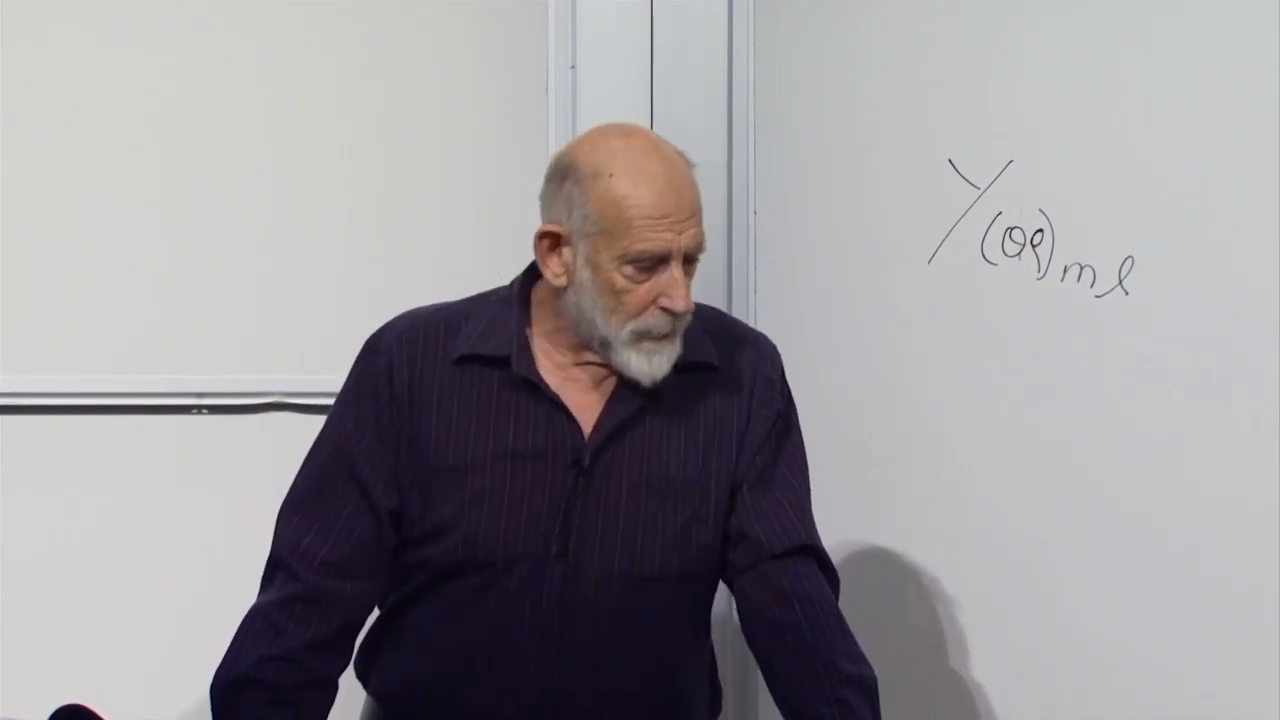
\includegraphics[width=0.9\linewidth]{lecture_03_frame_02.png}
\caption{固定經典角動量後，徑向哈密頓量包含徑向動能、離心項\(L^2/(2mr^2)\)和中心勢\(V(r)\)。}
\lectureframe{00:47:15}
\end{figure}

\(1/r^2\)項就是離心勢壘。粒子越接近原點，這一項越大，因此相應的力指向外。對於此處討論的類庫侖吸引勢，當\(L\neq0\)時，軌跡會繞著中心轉，而不會抵達中心。當\(L=0\)時，勢壘便不存在。

對於吸引庫侖勢，
\begin{equation}
V(r)=-\frac{\kappa}{r},
\end{equation}
在\(r\)較小處，離心項占優勢；庫侖項衰減得較慢，因此在\(r\)較大處占優勢。當\(L\neq0\)時，兩項之和有一個極小值。粒子在極小值處運動時，半徑保持不變，因此軌道是圓形。能量高於極小值、低於逃逸閾值的束縛運動，會在最小半徑和最大半徑之間來回振盪；在庫侖問題中，這就是橢圓軌道的徑向振盪。

\section{約化徑向方程}

量子力學中，具有確定軌道角動量的態，其角度部分是球諧函數。將分離變數後的態寫成
\begin{equation}
\Psi_{n_r\ell m}(r,\theta,\phi)
=\frac{u_{n_r\ell}(r)}{r}\,
Y_{\ell m}(\theta,\phi).
\end{equation}
角算符\(L^2\)的本徵值為
\begin{equation}
L^2Y_{\ell m}
=\hbar^2\ell(\ell+1)Y_{\ell m}.
\end{equation}
固定\(n_r,\ell\)後，將\(u_{n_r\ell}(r)\)簡寫為\(u(r)\)。剩下的約化徑向函數滿足方程
\begin{equation}
\begin{aligned}
&-\frac{\hbar^2}{2m}\frac{d^2u}{dr^2}
+\frac{\hbar^2\ell(\ell+1)}{2mr^2}u(r)\\
&\qquad+V(r)u(r)=E_{n_r\ell}\,u(r).
\end{aligned}
\end{equation}

\editorialnote{純粹的一維二階導數方程使用約化徑向函數\(u=rR\)。因此，講課方程中顯示的\(\psi(r)\)對應於\(u(r)\)；而在\(\Psi=R(r)Y_{\ell m}\)中，普通的徑向因子是\(R=u/r\)。採用這種寫法，可避免把\(-i\hbar\,d/dr\)當成三維徑向希爾伯特空間上的獨立厄米徑向動量算符。}

下方黑板上顯示的是約化徑向方程。\footnote{來源影格：\texttt{\detokenize{lecture_03_frame_03.png}}，講課影片時間\(00{:}54{:}32\)。}

\begin{figure}[htbp]
\centering
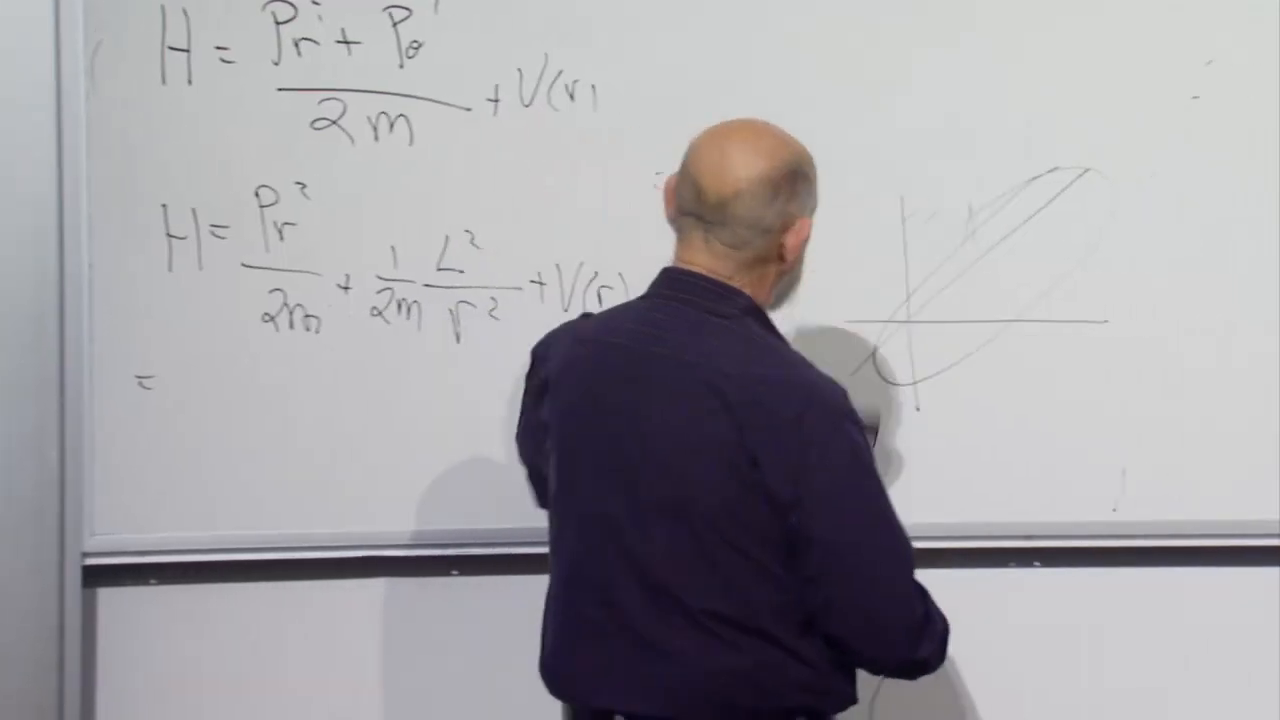
\includegraphics[width=0.9\linewidth]{lecture_03_frame_03.png}
\caption{固定\(\ell\)後，約化徑向波函數滿足一維Schr\"odinger方程，其中包含一個正比於\(\ell(\ell+1)/r^2\)的離心項。}
\lectureframe{00:54:32}
\end{figure}

三維角度結構的影響已濃縮在參數\(\ell\)中。徑向方程不含磁量子數\(m\)。

\begin{classroomqa}
\lecturetimestamp{00:55:34}
\audiencequestion{給定\(\ell\)後，\(2\ell+1\)個磁量子數態的能量是否相同？}
\lecturerresponse{是，只要徑向本徵態也固定即可。對每個選定的\(u_{n_r\ell}\)，所有\(m=-\ell,\ldots,\ell\)取值的態能量都相同，因為\(m\)不會出現在徑向方程中。同一\(\ell\)下，不同徑向本徵態的能量通常不同。}
\end{classroomqa}

\begin{classroomqa}
\lecturetimestamp{00:56:03}
\audiencequestion{為什麼可以用\(\hbar^2\ell(\ell+1)\)取代\(L^2\)？\(\ell\)與\(m\)的允許值有何關係？}
\lecturerresponse{數值\(\ell\)用來標記一個角動量多重態，也是該多重態中\(m\)的最大值。多重態中的每個態都具有相同的\(L^2\)本徵值\(\hbar^2\ell(\ell+1)\)，因此將此本徵值代入徑向方程。}
\end{classroomqa}

此處的論證不需要特殊函數解的明確形式。重要的是了解這些解如何排列。

\section{徑向節點與能階}

固定\(\ell\)後，約化徑向方程就是一個普通的一維本徵值問題。束縛態依內部節點數目排列。最低徑向態沒有內部節點，下一個有一個，再下一個有兩個。節點越多，波函數變化越快；變化越快，動量越大，因此動能也越大。

每個\(\ell\)取值都對應不同的徑向算符，因為離心項會隨\(\ell\)改變。因此，\(\ell=0,1,2,\ldots\)各自形成一系列徑向能階。隨角動量增加，正的離心項會使能階上移。固定\(\ell\)後，每個徑向本徵值都對應一個維度為
\begin{equation}
2\ell+1.
\end{equation}
的磁量子數多重態。\(\ell=0\)能階是單重態，\(\ell=1\)能階是三重態，\(\ell=2\)能階是五重態。這些簡併是旋轉對稱性所保證的；額外的對稱性也可能使不同\(\ell\)的態具有相同能量。

對於在\(r\)很大時滿足\(V(r)\to0\)的原子型勢，逃逸閾值依慣例取為\(E=0\)。能量為負的態構成離散束縛譜。在\(E=0\)及其以上則是散射連續譜。這項敘述取決於勢在\(r\)很大時的行為，因此不適用於具束縛作用的中心勢。

\section{特殊的庫侖簡併}

精確的非相對論庫侖勢還會使能階呈現另一種對應關係。最低的\(\ell=1\)徑向態與第一激發\(\ell=0\)態能量相同。下一個\(\ell=1\)態與第二激發\(\ell=0\)態能量相同，而最低的\(\ell=2\)態也與它們能量相同。這種模式會延續到更高的徑向與角動量能階序列。

\begin{classroomqa}
\lecturetimestamp{01:09:57}
\audiencequestion{這種額外的庫侖簡併是否代表另一種對稱性？}
\lecturerresponse{是。這是精確庫侖勢所具有的一種特殊額外對稱性。勢稍有變化，這種能階對應關係就會消失；此處不推導這種對稱性。}
\end{classroomqa}

由此得到的軌道殼層簡併度為
\begin{equation}
1,\qquad 4,\qquad 9,\qquad 16,\qquad \ldots
\end{equation}
這還未計入電子自旋。

\begin{classroomqa}
\lecturetimestamp{01:11:46}
\audiencequestion{這種簡併適用於氫原子，還是只適用於理想庫侖問題？}
\lecturerresponse{氫原子非常接近這種情形，但並非完全如此。相對論修正與原子核的有限大小都會擾動理想庫侖能階排列。}
\end{classroomqa}

點原子核產生精確的\(1/r\)勢。若原子核的電荷分布在一個小體積內，電子進入該體積時所受的勢就會略有不同；即使這個偏差很小，也會解除部分特殊簡併。

此處也尚未計入自旋。計入電子的兩種自旋態後，殼層態數加倍為
\begin{equation}
2,\qquad 8,\qquad 18,\qquad 32,\qquad \ldots
\end{equation}
這還未包含更完整原子理論所描述的進一步能階分裂。

\section{重新檢視笛卡兒座標下的方程}

徑向問題起始於三維定態Schr\"odinger方程：
\begin{equation}
\begin{aligned}
-\frac{\hbar^2}{2m}\nabla^2\Psi+V(r)\Psi&=E\Psi,\\
\nabla^2&=\frac{\partial^2}{\partial x^2}
+\frac{\partial^2}{\partial y^2}
+\frac{\partial^2}{\partial z^2},\\
r&=\sqrt{x^2+y^2+z^2}.
\end{aligned}
\end{equation}
改用徑向與角度座標，並選取\(L^2\)的本徵態。接著以\(\hbar^2\ell(\ell+1)\)取代\(L^2\)，便能將偏微分方程化約為前述的常微分徑向方程。

\begin{classroomqa}
\lecturetimestamp{01:16:42}
\audiencequestion{能否利用理想庫侖能譜的偏差來測定原子核大小？}
\lecturerresponse{無法只靠這種簡單比較來測定。其他修正大得多，必須先納入考量。此處提到原子核大小，是因為它是偏離點庫侖勢的一個直接例子。}
\end{classroomqa}

\begin{classroomqa}
\lecturetimestamp{01:17:09}
\audiencequestion{經典與量子角動量項的主要差異是什麼？}
\lecturerresponse{經典力學中，\(L^2\)是守恆向量大小的普通平方。在量子軌道多重態中，它的本徵值是\(\hbar^2\ell(\ell+1)\)，而不只是\(\hbar^2\ell^2\)。多出的那一項源自角動量分量不對易。}
\end{classroomqa}

\begin{classroomqa}
\lecturetimestamp{01:17:58}
\audiencequestion{束縛態波函數的支集是否為緊集？}
\lecturerresponse{不是。波函數會延伸到離中心任意遠處。對於此處討論的原子束縛態，波函數在遠處呈指數衰減，所以機率會變得微不足道，但在任何有限半徑之外都不會完全為零。}
\end{classroomqa}

\begin{classroomqa}
\lecturetimestamp{01:18:48}
\audiencequestion{當\(\ell=0\)使離心勢阱消失後，穩定點會如何變化？}
\lecturerresponse{離心勢壘與吸引力之間的競爭不再形成極小值。在點庫侖勢的理想化模型中，經典粒子會朝奇異中心運動。量子力學中，最低態不可能同時具有確定在中心的位置和零動量，因此最低態波函數會有有限的空間展寬。}
\end{classroomqa}

\editorialnote{對於正則的中心勢，經典零角動量軌跡可以穿過原點繼續運動。對於理想點庫侖勢，\(r=0\)則是碰撞奇點；若要延續經典軌跡，就需要另外訂定處理方式。}

經典力學的化約將單一軌道置於一個平面內，但量子波函數不能以同樣方式處理。量子軌道態遍布三維空間。完整的角動量算符為\(L^2=L_x^2+L_y^2+L_z^2\)，其本徵值保留了三維的結果\(\hbar^2\ell(\ell+1)\)。

\begin{classroomqa}
\lecturetimestamp{01:21:30}
\audiencequestion{經典軌道置於平面後，量子問題為何仍是三維的？}
\lecturerresponse{只有經典軌道被置於固定平面內：選取垂直於守恆角動量向量的座標即可做到。量子波函數仍佔據三維空間。其他角動量分量仍透過\(L^2\)保留下來，因此徑向方程包含\(\ell(\ell+1)\)，而不是只有單一分量的平方。}
\end{classroomqa}

\begin{classroomqa}
\lecturetimestamp{01:22:54}
\audiencequestion{每個量子問題都有升降算符嗎？}
\lecturerresponse{沒有。只有在一些特別有利的情況下才會出現升降算符。角動量問題是其中一例，諧振子問題則是另一例。諧振子的例子特別有用，因為穩定平衡附近的運動往往近似簡諧運動，包括有效勢極小值附近的小幅徑向振盪。}
\end{classroomqa}

此處先暫擱原子問題，接著以諧振子為例，說明如何利用階梯算符決定能譜。

\section{小振動與諧振子}

在穩定平衡附近，足夠小的位移往往會產生簡諧運動。非零角動量時的有效徑向勢就是一例：在勢阱底部附近，徑向運動近似為簡諧運動。

考慮質量為一的一維振子。令\(x\)表示偏離平衡位置的位移，並以\(k=\omega^2\)表示彈簧常數。經典哈密頓量為
\begin{equation}
H=\frac{p^2}{2}+\frac{\omega^2x^2}{2}.
\end{equation}
由哈密頓方程可得
\begin{equation}
\dot{x}=\frac{\partial H}{\partial p}=p,
\qquad
\dot{p}=-\frac{\partial H}{\partial x}=-\omega^2x,
\end{equation}
因此
\begin{equation}
\ddot{x}=-\omega^2x.
\end{equation}
所以\(\omega\)就是經典振盪頻率。

\section{因式分解與零點能}

量子力學中，
\begin{equation}
[x,p]=i\hbar.
\end{equation}
哈密頓量由平方項相加而成，因此可以嘗試以下因式分解：
\begin{align}
\frac{1}{2}(p+i\omega x)(p-i\omega x)
&=\frac{1}{2}\left(p^2+\omega^2x^2+i\omega[x,p]\right) \\
&=\frac{1}{2}\left(p^2+\omega^2x^2-\hbar\omega\right).
\end{align}
於是
\begin{equation}
H=\frac{1}{2}(p+i\omega x)(p-i\omega x)
+\frac{1}{2}\hbar\omega.
\end{equation}
加上的項\(\hbar\omega/2\)就是零點能。

經典力學中，最低能量會出現在\(x=p=0\)。量子力學中，沒有任何態能同時將位置和動量精確固定為零。此外，\(p^2/2\)與\(\omega^2x^2/2\)兩項都是正的，無法互相抵消。因此，基態能量必定不為零。

進行階梯算符計算時，可以先暫時略去共同的加性常數，最後再加回去。

\begin{classroomqa}
\lecturetimestamp{01:36:10}
\audiencequestion{零點能項為正，是否還能告訴我們其他事情？}
\lecturerresponse{振子哈密頓量是正算符：它是正平方項的總和，因此能量不可能為負。}
\end{classroomqa}

\section{振子階梯}

引入無因次算符。\footnote{在\(01{:}37\)--\(01{:}42\)附近的推導中，取\(\hbar=1\)。在這些歸一化定義中加回\(\hbar\)因子，使\(A_\pm\)成為無因次量，且其對易子為一。}
\begin{equation}
A_+=\frac{p+i\omega x}{\sqrt{2\hbar\omega}},
\qquad
A_-=\frac{p-i\omega x}{\sqrt{2\hbar\omega}}.
\end{equation}
它們互為厄米共軛：
\begin{equation}
A_+^\dagger=A_-.
\end{equation}
它們的對易子為
\begin{align}
[A_-,A_+]
&=\frac{1}{2\hbar\omega}
\left([p,i\omega x]+[-i\omega x,p]\right) \\
&=1.
\end{align}

定義
\begin{equation}
N=A_+A_-.
\end{equation}
哈密頓量便是
\begin{equation}
H=\hbar\omega\left(N+\frac{1}{2}\right).
\end{equation}
因此，求能譜就化約為求\(N\)的本徵值。

假設
\begin{equation}
N|n\rangle=n|n\rangle.
\end{equation}
與\(N\)的對易關係為\footnote{在\(01{:}45{:}37\)--\(01{:}48{:}10\)處的中間步驟，是直接根據已給出的關係\(N=A_+A_-\)和\([A_-,A_+]=1\)重建的。}
\begin{align}
[N,A_+]
&=A_+[A_-,A_+]=A_+, \\
[N,A_-]
&=[A_+,A_-]A_-=-A_-.
\end{align}
因此可得
\begin{align}
N\bigl(A_+|n\rangle\bigr)
&=(n+1)A_+|n\rangle, \\
N\bigl(A_-|n\rangle\bigr)
&=(n-1)A_-|n\rangle.
\end{align}
只要所得向量不為零，\(A_+\)就會使\(N\)的本徵值增加一，而\(A_-\)則會使它減少一。

算符\(N\)是非負的：
\begin{equation}
\langle\psi|N|\psi\rangle
=\langle\psi|A_+A_-|\psi\rangle
=\|A_-|\psi\rangle\|^2
\geq0.
\end{equation}
因此，降階過程不可能繼續到負本徵值。在底態\(|b\rangle\)處，這個過程必須終止：
\begin{equation}
A_-|b\rangle=0.
\end{equation}

對歸一化本徵態而言，階梯上的係數由範數決定：
\begin{align}
\|A_-|n\rangle\|^2
&=\langle n|A_+A_-|n\rangle=n, \\
\|A_+|n\rangle\|^2
&=\langle n|A_-A_+|n\rangle=n+1.
\end{align}
因此可以選擇相位，使得
\begin{equation}
A_-|n\rangle=\sqrt{n}\,|n-1\rangle,
\qquad
A_+|n\rangle=\sqrt{n+1}\,|n+1\rangle.
\end{equation}

\begin{classroomqa}
\lecturetimestamp{01:52:42}
\audiencequestion{如果\(A_-\)使一個態降低，而\(A_+\)又把它升回去，那麼\(A_+A_-\)怎麼會得到本徵值\(n\)？}
\lecturerresponse{階梯算符作用時會帶有歸一化因子。先作用\(A_-\)會帶來因子\(\sqrt n\)；接著對所得態作用\(A_+\)，又會帶來因子\(\sqrt n\)。兩者相乘就是\(n\)。}
\end{classroomqa}

確實，
\begin{equation}
A_+A_-|n\rangle
=\sqrt n\,A_+|n-1\rangle
=n|n\rangle.
\end{equation}

\begin{classroomqa}
\lecturetimestamp{01:55:52}
\audiencequestion{\(N\)的最低本徵值必須是零嗎？它也可能是正值嗎？}
\lecturerresponse{最低本徵值必定是零，而\(N\)的譜由非負整數構成。此處尚未證明這個端點結果。}
\end{classroomqa}

\editorialnote{令\(|b\rangle\)為最低態。由於降階過程必須終止，\(A_-|b\rangle=0\)。因此立即可得\(N|b\rangle=A_+A_-|b\rangle=0\)，所以\(N\)的最低本徵值為零。}

從這個最低態出發，作用\(A_+\)可得
\begin{equation}
n=0,1,2,\ldots.
\end{equation}
加回零點能這個加性項後，振子的能量為
\begin{equation}
E_n=\hbar\omega\left(n+\frac{1}{2}\right),
\qquad n=0,1,2,\ldots.
\end{equation}

接下來會進一步發展振子代數，並用它來求解其他量子問題。
\chapter{振子波函數、自旋二分之一與粒子交換}

\section{無所不在的振子}

任何具有穩定平衡位置的系統，受到偏離平衡位置的擾動時都可能振盪。它可能只有一個頻率，也可能有許多頻率。例如，小提琴弦有基音模態和更高次的諧波。撥動琴弦會激發這些模態的某種組合。

這裡更重要的例子是場。電磁場的平衡態是真空：沒有電場、沒有磁場，也沒有電磁振盪。將輻射導入腔體或波導後，場可以在其允許的模態中振盪，每個模態都有自己的頻率。在量子理論中，這些模態描述的是光子的集合。

同樣的想法也適用於晶體。若把每個原子都想成獨立的振子，便會產生誤解。原子彼此施力，因此一個原子的位移會影響鄰近原子，波也會在晶體中傳播。這種耦合運動的正規模態是諧振子，其量子稱為聲子。光子和聲子是不同的物理對象，但兩者都可歸結為相同的振子代數。

\section{振子代數}

討論振子時，令質量和約化普朗克常數都等於一：
\[
m=1,\qquad \hbar=1.
\]
哈密頓量為
\begin{equation}
H=\frac{p^{2}}{2}+\frac{\omega^{2}x^{2}}{2}.
\end{equation}
參數\(\omega\)決定勢能的曲率，也就是振盪頻率。

定義升算符和降算符如下：
\begin{equation}
A_{\pm}=\frac{p\pm i\omega x}{\sqrt{2\omega}}.
\end{equation}
其正規化方式使得
\begin{equation}
[A_{-},A_{+}]=1.
\end{equation}
數算符為
\begin{equation}
N=A_{+}A_{-}.
\end{equation}
這些方程合起來表示，\(A_{+}\)會使\(N\)的本徵值增加一，而\(A_{-}\)會使之減少一。因此，能譜為
\begin{equation}
n=0,1,2,3,\ldots .
\end{equation}

將兩個階梯算符相乘，也可看出經典能量的量子修正：
\begin{align}
N
&=\frac{1}{2\omega}(p+i\omega x)(p-i\omega x)\\
&=\frac{1}{2\omega}\left(p^{2}+\omega^{2}x^{2}
 +i\omega[x,p]\right)\\
&=\frac{1}{2\omega}\left(p^{2}+\omega^{2}x^{2}-\omega\right),
\end{align}
其中\([x,p]=i\)。因此，
\begin{equation}
H=\omega\left(N+\frac12\right).
\end{equation}
若附加常數與問題無關，使用平移後的哈密頓量會較方便：
\begin{equation}
H_{\mathrm{shifted}}=H-\frac{\omega}{2}=\omega N.
\end{equation}
項\(\omega/2\)是振子的零點能，也就是基態能量。對場模態而言，相應的項稱為真空能。它反映了不確定性原理：沒有任何態能讓\(x\)和\(p\)同時精確等於零，因此\(H\)中的兩個正二次項，其期望值不可能同時為零。

\begin{classroomqa}
\lecturetimestamp{00:09:46}
\audiencequestion{為什麼數算符的譜包含零？}
\lecturerresponse{可以藉由明確構造基態波函數來證明。這個構造會找出一個滿足\(N=0\)的態。}
\end{classroomqa}

要開始這個構造，可以用位置波函數取代態向量。能量本徵態變成
\[
\psi_{0}(x),\ \psi_{1}(x),\ \psi_{2}(x),\ldots,
\]
而基本算符的作用方式為
\begin{equation}
X\longmapsto x,\qquad
P\longmapsto -i\frac{d}{dx}.
\end{equation}
恢復\(\hbar\)後，第二個替換應為
\(P\mapsto-i\hbar\,d/dx\)。

在求解\(\psi_{0}\)之前，這個問題有個更快的抽象解答。在可正規化振子本徵態構成的離散階梯上，\(N=A_{+}A_{-}\)是非負的，因此不可能以單位步長無限地反覆降低。在階梯底端---其可正規化波函數將於下文構造---處，必定有一個態，記為\(\lvert0\rangle\)，滿足
\begin{equation}
A_{-}\lvert0\rangle=\mathbf 0.
\end{equation}
否則，\(A_{-}\lvert0\rangle\)會是再低一階的另一個態。立即可得
\begin{equation}
N\lvert0\rangle
=A_{+}A_{-}\lvert0\rangle
=\mathbf 0
=0\,\lvert0\rangle.
\end{equation}
因此，底端態的數本徵值為零。

\begin{classroomqa}
\lecturetimestamp{00:14:57}
\audiencequestion{若本徵值是零，等式右側是否應該是零本徵向量？}
\lecturerresponse{右矢\(\lvert0\rangle\)是正規化的非零向量，其標記為零。在\(N\lvert0\rangle=0\,\lvert0\rangle\)中，等式右側是零向量。基態右矢和零向量是不同的對象。}
\end{classroomqa}

\section{薛丁格Schr\"odinger方程與物理解}

現在回到位置表象。不含時的Schr\"odinger方程為
\begin{equation}
\left[
-\frac12\frac{d^{2}}{dx^{2}}
+\frac12\omega^{2}x^{2}
\right]\psi(x)=E\psi(x).
\end{equation}
作為一個二階微分方程，它對任意\(E\)值都有形式解。但其中大多數形式解都不是物理上可接受的振子態；它們在\(\lvert x\rvert\)很大時會指數增長，使其範數發散。

束縛態的波函數必須平方可積：
\begin{equation}
\int_{-\infty}^{\infty}\psi^{*}(x)\psi(x)\,dx<\infty.
\end{equation}
如此一來，就可以將波函數正規化，使積分等於一。只有特定的能量值才會產生這類解。無限直線上的位置態和動量態在這方面是例外；至於指數增長的振子解，則直接排除於態空間之外。

\section{高斯基態}

這個二階方程可以求解，但利用階梯代數可得到更簡單的一階方程：
\begin{equation}
A_{-}\psi_{0}(x)=0.
\end{equation}
等式右側為零時，\(A_{-}\)的整體因子不影響結果，因此這等價於
\begin{equation}
(p-i\omega x)\psi_{0}(x)=0.
\end{equation}
利用\(p=-i\,d/dx\)可得
\begin{equation}
\left(\frac{d}{dx}+\omega x\right)\psi_{0}(x)=0.
\end{equation}

\begin{classroomqa}
\lecturetimestamp{00:22:32}
\audiencequestion{可以用變數分離法求解嗎？}
\lecturerresponse{只有一個自變數，沒有兩個變數可以分離。把方程寫成\(\psi_{0}'/\psi_{0}=-\omega x\)的形式，就能看出它是對數導數。這提示我們將波函數寫成指數形式。}
\end{classroomqa}

一種簡便的解法是令
\begin{equation}
\psi_{0}(x)=e^{f(x)}.
\end{equation}
於是
\[
\psi_{0}'(x)=f'(x)e^{f(x)},
\]
約去兩邊相同的指數因子後，方程化為
\begin{equation}
\frac{df}{dx}+\omega x=0.
\end{equation}

\begin{classroomqa}
\lecturetimestamp{00:26:28}
\audiencequestion{\(f(x)\)裡應該有一個負號嗎？}
\lecturerresponse{是的。由於\(df/dx=-\omega x\)，積分後會得到負的二次項。}
\end{classroomqa}

因此
\begin{equation}
f(x)=-\frac12\omega x^{2}+C,
\end{equation}
而且
\begin{equation}
\psi_{0}(x)\propto e^{-\omega x^{2}/2}.
\end{equation}
乘法正規化常數不必明確指定。關鍵在於其高斯形狀：波函數平滑、集中在原點附近，並在\(\lvert x\rvert\)很大時迅速衰減。顯然它是平方可積的。

無須將答案代回二階方程，就能求出其能量。代數已經給出
\begin{equation}
E_{0}=\frac{\omega}{2}.
\end{equation}

\section{激發態、節點與經典運動}

對基態作用升算符，即可得到第一激發態：
\begin{equation}
\psi_{1}(x)\propto A_{+}\psi_{0}(x)
\propto(p+i\omega x)e^{-\omega x^{2}/2}.
\end{equation}
基態方程給出
\[
p\psi_{0}=i\omega x\,\psi_{0}.
\]
改變階梯算符中的符號，就會把相消變成相加：
\begin{equation}
(p+i\omega x)\psi_{0}
=2i\omega x\,\psi_{0}.
\end{equation}
略去整體常數後，
\begin{equation}
\psi_{1}(x)\propto x\,e^{-\omega x^{2}/2}.
\end{equation}

這個波函數是奇函數：
\begin{equation}
\psi_{1}(-x)=-\psi_{1}(x).
\end{equation}
它的機率密度是偶函數，但在原點有一個節點：
\begin{equation}
\lvert\psi_{1}(0)\rvert^{2}=0.
\end{equation}
因此，第一激發態的機率密度在\(x=0\)有一個節點。

反覆作用\(A_{+}\)，會得到乘上相同高斯包絡的高次多項式。\footnote{講課中說明，高次多項式因子每升一階便多一個節點，對稱性則從\(00{:}34{:}25\)到\(00{:}35{:}49\)交替變化。Leonard Susskind 與 Art Friedman 在\emph{Quantum Mechanics: The Theoretical Minimum}（2014）討論振子本徵函數時，也印證了高斯函數乘上多項式的形式。}略去正規化因子後，
\begin{equation}
\psi_{n}(x)=P_{n}(x)e^{-\omega x^{2}/2}.
\end{equation}
宇稱在偶與奇之間交替，每升一階便增加一個節點。隨著\(n\)增大，波函數會延伸到離原點更遠處，並且振盪得更快。

這兩個特徵都有直接的物理意義。波函數延伸到離原點更遠處，表示勢能較大，因為勢能隨\(x^{2}\)增加。位置空間中的快速振盪則代表較大的動量。高度激發的振子更可能到達離中心較遠處；它通過中心區域時，動量較大，波函數在該處也振盪得更快。

\begin{classroomqa}
\lecturetimestamp{00:37:18}
\audiencequestion{當\(n\)變大時，諧振子會不會仍無法呈現經典行為？}
\lecturerresponse{經典運動並非由單一定態能量本徵態表示，而是出現在包含許多能階的波包中。例如，位移後的高斯波包會像經典振子一樣來回運動；而擺動幅度越大，相對不確定度就越小。}
\end{classroomqa}

從基態高斯波包開始，將它從原點平移開來。平移後的波包不再是能量本徵態，而是許多能量本徵態的疊加。在含時Schr\"odinger方程的演化下，各分量會獲得不同的相位。波包在勢能的一側和另一側之間往返，在中心附近產生快速的相位變化，到了轉折點附近則再次變得平滑。相較於波包的寬度，位移越大，運動就越接近經典情況。

\begin{classroomqa}
\lecturetimestamp{00:39:29}
\audiencequestion{第二激發態的波函數是否應該在原點為零？}
\lecturerresponse{不會。它的多項式因子不只是\(x^{2}\)，還包含一個常數項，因此波函數不一定在\(x=0\)為零。}
\end{classroomqa}

階梯論證也假設\(A_{+}\)和\(A_{-}\)在振子的平方可積函數定義域上互為厄米共軛，並滿足伴隨關係所需的邊界條件。指數增長的形式解不屬於這個定義域。

\begin{classroomqa}
\lecturetimestamp{00:40:45}
\audiencequestion{有沒有通用的方法，能判斷哪些哈密頓量可以用這些代數方法求解？}
\lecturerresponse{沒有這樣的通用規則。精確可解的例子很少。諧振子和理想的非相對論氫原子是少數能用代數方法求解的例子。}
\end{classroomqa}

\section{自旋二分之一作為角動量}

自旋是粒子本身攜帶的角動量，與其質心的軌道運動無關。靜止的粒子沒有軌道角動量\(\mathbf R\times\mathbf P\)，但仍可能有自旋。可以試著把它想像成微小的旋轉物體，也可以把自旋視為內禀的量子性質。關鍵的陳述在於數學形式：自旋的分量會隨空間旋轉而變換，並遵守角動量對易關係。

從此處起恢復\(\hbar\)。角動量分量滿足
\begin{equation}
[L_{z},L_{x}]=i\hbar L_{y},
\end{equation}
另外兩個關係可由循環置換得到。無因次的泡利矩陣為
\begin{equation}
\begin{aligned}
\sigma_{z}&=
\begin{pmatrix}
1&0\\
0&-1
\end{pmatrix},\\[0.4em]
\sigma_{x}&=
\begin{pmatrix}
0&1\\
1&0
\end{pmatrix},\\[0.4em]
\sigma_{y}&=
\begin{pmatrix}
0&-i\\
i&0
\end{pmatrix}.
\end{aligned}
\end{equation}
在這個基底中，\(\sigma_{z}\)是對角矩陣，其本徵值為\(+1\)和
\(-1\)。

\begin{classroomqa}
\lecturetimestamp{00:47:35}
\audiencequestion{\(\sigma_x\)裡有負號嗎？}
\lecturerresponse{沒有。\(\sigma_x\)的兩個非對角元素都是正的。}
\end{classroomqa}

\(00{:}49{:}35\)的板書計算從逐項相乘開始。完成矩陣乘法後可得
\begin{align}
\sigma_{z}\sigma_{x}
&=
\begin{pmatrix}
0&1\\
-1&0
\end{pmatrix}
=i\sigma_{y},\\
\sigma_{x}\sigma_{z}
&=
\begin{pmatrix}
0&-1\\
1&0
\end{pmatrix}
=-i\sigma_{y}.
\end{align}
因此
\begin{equation}
[\sigma_{z},\sigma_{x}]=2i\sigma_{y}.
\end{equation}
定義物理自旋算符時加入下式，即可消去多出的因子二。\footnote{板書計算省略了\(\hbar\)；此處將它補回，使\(S_i\)具有角動量的單位。}
\begin{equation}
S_{i}=\frac{\hbar}{2}\sigma_{i}.
\end{equation}
於是
\begin{equation}
[S_{z},S_{x}]=i\hbar S_{y},
\end{equation}
循環置換的情形也相同。因此，將\(\hbar\)因子補回後，半個泡利矩陣便構成一組角動量算符。

令\(\hbar=1\)，即可得到如下形式。\footnote{來源影格為\texttt{lecture\_04\_frame\_02.png}。}
\begin{figure}[htbp]
\centering
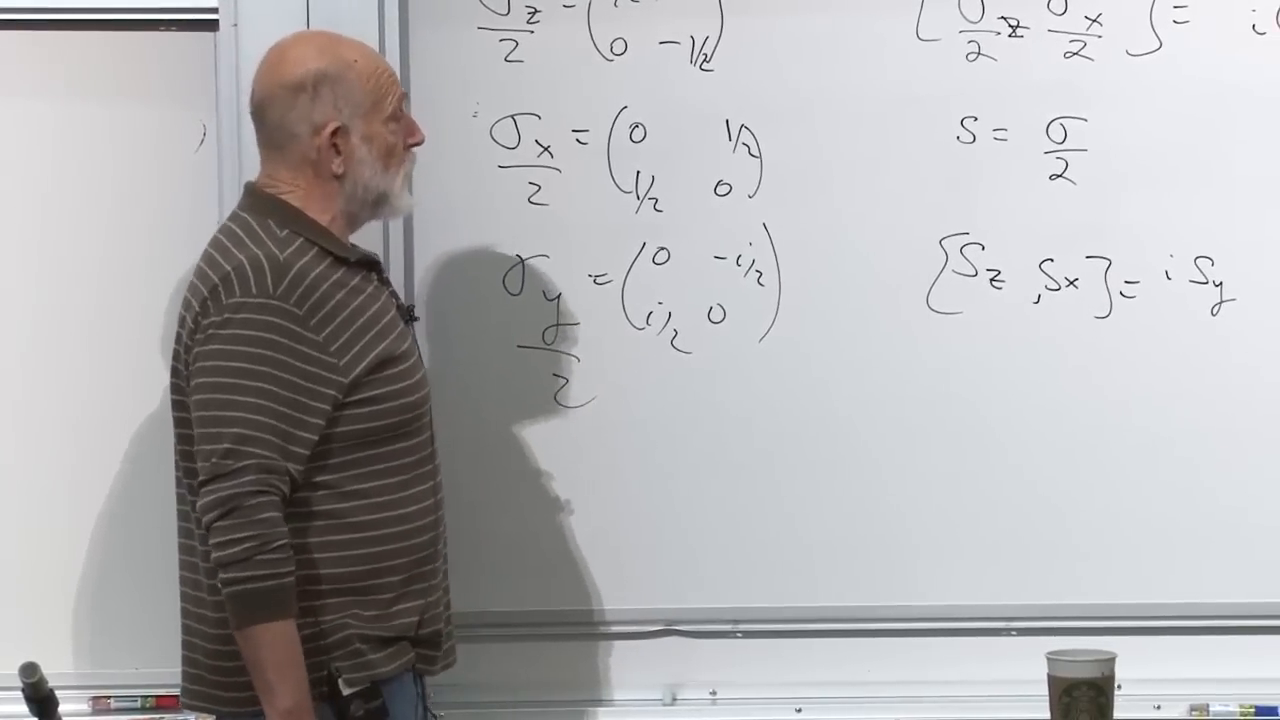
\includegraphics[width=0.9\linewidth]{lecture_04_frame_02.png}
\caption{在\(\hbar=1\)的單位制下，泡利矩陣的一半是自旋二分之一的角動量算符，並滿足\([S_z,S_x]=iS_y\)。}
\lectureframe{00:55:41}
\end{figure}

兩個\(S_z\)本徵值方程為
\begin{equation}
S_z\lvert\pm\rangle
=\pm\frac{\hbar}{2}\lvert\pm\rangle.
\end{equation}
等價地，無因次的磁量子數為
\begin{equation}
m_{s}=\pm\frac12,
\qquad
S_{z}\lvert m_{s}\rangle
=m_{s}\hbar\,\lvert m_{s}\rangle.
\end{equation}
角動量升、降算符會使\(m\)以整數步長改變，但這不表示每個階梯都必須經過零。整數多重態包含整數\(m\)值，半整數多重態則包含半整數值。自旋二分之一的階梯只有\(m_s=+1/2\)和\(m_s=-1/2\)兩個態。

這兩個態構成自旋二分之一的雙重態。電子、{\proseunicodefont μ}子、中微子和夸克都是以這類半整數自旋多重態描述的粒子。

\section{軌道角動量與自旋角動量}

現在有兩種角動量。軌道角動量描述相對於原點的運動：
\begin{equation}
\mathbf L=\mathbf R\times\mathbf P,
\end{equation}
而\(\mathbf S\)是內禀自旋。兩者的向量和就是總角動量：
\begin{equation}
\mathbf J=\mathbf L+\mathbf S.
\end{equation}

\begin{classroomqa}
\lecturetimestamp{00:56:49}
\audiencequestion{若系統的總角動量為\(\mathbf J\)，要如何判定它的自旋\(\mathbf S\)？}
\lecturerresponse{自旋量子數和軌道量子數通常會分別給定。若\(L=0\)，所有角動量都是自旋；否則就需要用到角動量相加的量子規則，這裡暫不討論。}
\end{classroomqa}

角動量相加規則同樣適用於軌道角動量與自旋相加、兩個自旋相加，或兩個軌道角動量相加。組合後的系統有自己的總角動量允許值，但目前還不需要用到這些規則。

\begin{classroomqa}
\lecturetimestamp{00:58:18}
\audiencequestion{什麼實驗證據促使物理學家引入自旋？}
\lecturerresponse{光譜學提供了證據；不過，元素週期表的殼層結構尤其清楚地說明了引入自旋的理由：電子必須具有額外的二值性質。}
\end{classroomqa}

\section{類氫能階簡併與殼層計數}

軌道角動量的\(L^{2}\)本徵值方程為
\begin{equation}
L^{2}\lvert\ell,m\rangle
=\hbar^{2}\ell(\ell+1)\lvert\ell,m\rangle,
\end{equation}
固定的\(\ell\)值對應
\begin{equation}
2\ell+1
\end{equation}
個磁態，其磁量子數為\(m=-\ell,-\ell+1,\ldots,\ell\)。

理想的非相對論庫侖問題還有額外的簡併。束縛態能量為負，並由下方趨近於零；但計數時只需關注能階的對應關係。第一個\(\ell=1\)能階與下一個\(\ell=0\)能階重合；第一個\(\ell=2\)能階則與下一個主殼層中的能階重合；此模式依此延續。\footnote{\texttt{lecture\_04\_frame\_03.png}，見\(01{:}02{:}01\)；完整的主殼層能階對應則從\(01{:}02{:}33\)延續至\(01{:}04{:}10\)。}

\begin{figure}[htbp]
\centering
\begin{tikzpicture}[x=1.55cm,y=1.0cm]
\draw[->] (-0.65,0) -- (-0.65,4.35);
\draw[->] (-0.85,0) -- (4.75,0);
\node at (-0.95,4.08) {\(E\)};
\node at (4.55,-0.28) {\(\ell\)};
\node at (0,-0.30) {\(0\)};
\node at (2,-0.30) {\(1\)};
\node at (4,-0.30) {\(2\)};

\draw (-0.20,0.75) -- (0.20,0.75);

\draw (-0.20,2.00) -- (0.20,2.00);
\foreach \dx in {-0.18,0,0.18}
  \draw (2+\dx-0.06,2.00) -- (2+\dx+0.06,2.00);

\draw (-0.20,3.15) -- (0.20,3.15);
\foreach \dx in {-0.18,0,0.18}
  \draw (2+\dx-0.06,3.15) -- (2+\dx+0.06,3.15);
\foreach \dx in {-0.32,-0.16,0,0.16,0.32}
  \draw (4+\dx-0.05,3.15) -- (4+\dx+0.05,3.15);

\node[anchor=west] at (0.35,0.75) {\(n=1\)};
\node[anchor=west] at (2.35,2.00) {\(n=2\)};
\node[anchor=west] at (4.40,3.15) {\(n=3\)};
\end{tikzpicture}
\caption{前三個理想庫侖殼層中，具有相同主能量的軌道多重態合併在一起：第一個殼層有一個態，第二個殼層有\(1+3\)個，第三個殼層有\(1+3+5\)個。}
\lectureframe{01:02:01}
\end{figure}

在主殼層\(n\)中，允許的軌道角動量值為\footnote{這個簡潔的\(\ell\)範圍及下方的總和，重現了從\(01{:}02{:}33\)到\(01{:}04{:}10\)所述的能階對應關係，以及\(1,4,9,16,\ldots\)這組計數。能譜圖的開頭見\texttt{lecture\_04\_frame\_03.png}，時間點為\(01{:}02{:}01\)。}
\[
\ell=0,1,\ldots,n-1.
\]
因此，空間態的數目為
\begin{equation}
\sum_{\ell=0}^{n-1}(2\ell+1)=n^{2},
\end{equation}
依序為
\begin{equation}
1,\ 4,\ 9,\ 16,\ldots .
\end{equation}
這裡只計算軌道態。每個空間態都允許兩種自旋值，因此相應的理想化總數為
\begin{equation}
2,\ 8,\ 18,\ 32,\ldots=2n^{2}.
\end{equation}

\section{泡利不相容原理與電子的二值性質}

先考慮獨立電子近似下的氦原子。氦原子核的質子電荷是氫核的兩倍，因此類氫能階會重新縮放，電子也會被拉得更靠近原子核。暫且忽略電子--電子間的交互作用，兩個電子可以佔據最低的空間軌域，這是氦基態的一個合理初步近似。

為什麼不能再放入第三個電子？那會降低它的軌域能量，但實際上並不會如此。限制來自泡利不相容原理：兩個電子不能佔據相同的完整單粒子態。若把這稱為一般的排斥力，就會造成誤解；這其實是對允許量子態的限制。

這裡看似有個矛盾：兩個氦電子確實佔據同一個空間軌域。解答在於，完整的電子態不只有軌域波函數，還包含一個二值自由度，稱為自旋向上和自旋向下。一個電子可以在最低軌域中自旋向上，另一個則自旋向下；它們的空間態相同，但完整的量子態不同。

這裡先往前計算到鋰，再回頭推敲。這個回溯揭示了不相容原理和自旋為何缺一不可。假設不相容規則中完全沒有自旋，那麼只有一個電子能佔據最低空間態；第二個電子便得進入下一個主殼層中的四個空間態之一。如此會有好幾種可能的基態，但觀測到的氦基態卻是唯一的。因此，這種沒有自旋的不相容原理並不正確。

加回兩種自旋值後，兩個電子便以相反的自旋填入最低軌域。第三個電子（例如中性鋰原子的第三個電子）必須進入下一個主殼層。該殼層有一個\(\ell=0\)空間態和三個\(\ell=1\)空間態。在計入自旋之前，共有四種可能。

\begin{classroomqa}
\lecturetimestamp{01:14:58}
\audiencequestion{\(s\)態和\(p\)態如何在第一激發殼層中形成八種可能？}
\lecturerresponse{有一個\(\ell=0\)空間態和三個\(\ell=1\)空間態，共計四個空間態。每個空間態都允許兩種自旋值，因此總數是\(2(1+3)=8\)。}
\end{classroomqa}

元素週期表第二週期有八個元素，背後的簡單計數就是如此。這是刻意採用的理想化模型：後文會說明，電子--電子間的交互作用很快就會使獨立類氫殼層的圖像失效。

也可以透過角動量來檢驗這種二值性質。電子自旋伴隨磁矩，因此磁場會使兩種自旋投影的能量不同。原本在零磁場下簡併的能階會分裂成兩個，這正符合小磁矩順著或逆著磁場排列時的預期。這種能階分裂可檢驗新增的二值自由度是否具有角動量的性質，而非任意的二元標籤。

\section{光子、電子與殼層模型的適用範圍}

粒子並非都遵守相同的佔據規則。許多光子可以佔據同一個電磁模態；經典光波可以理解為該模態中含有大量光子的態。電子則不同：不相容原理禁止它們全都進入同一個完整量子態。這種差異引出了兩種粒子統計的區分。

\begin{classroomqa}
\lecturetimestamp{01:20:28}
\audiencequestion{如果是自由電子流，而非束縛在原子中的電子，情況會如何？}
\lecturerresponse{不相容規則仍然適用：電子不能全都佔據同一個量子態。雷射可以讓許多光子進入同一個模態，但電子流無法用這種方式製備。}
\end{classroomqa}

這項限制是電子本身的性質，並非原子束縛所特有。

\begin{classroomqa}
\lecturetimestamp{01:21:12}
\audiencequestion{軌道角動量是否特指繞著原子核旋轉？}
\lecturerresponse{角動量是相對於選定的原點來定義的。在原子中，原子核是自然的原點；自由粒子則相對於所選原點具有角動量\(\mathbf R\times\mathbf P\)。}
\end{classroomqa}

討論旋轉時，都要選定旋轉所繞的點。原子有自然的中心，因為原子核是近似中心勢的中心。在自由空間中，沒有特別優先的原點，但仍可相對於任意選定的原點計算角動量。

\begin{classroomqa}
\lecturetimestamp{01:22:34}
\audiencequestion{為什麼元素週期表會先有一列列重複的八個元素，之後又有一列列重複的十八個元素？}
\lecturerresponse{簡單的獨立電子殼層模型無法解釋完整的週期規律。由於忽略了電子間的交互作用，這個模型很快就會失效。}
\end{classroomqa}

對大型原子而言，外層電子不僅與原子核作用，也會與數量可觀的內層電子雲作用。若將每個電子都視為在未受遮蔽的庫侖場中獨立運動，便不再合理。

\begin{classroomqa}
\lecturetimestamp{01:23:33}
\audiencequestion{為什麼原子加入更多電子後，體積不會大幅增加？}
\lecturerresponse{加入電子的同時，原子核中的質子也會增加。核電荷增加會將內層電子往內拉，而內層電子又會遮蔽原子核。在這個簡化的圖像中，外層價電子感受到的有效電荷大約為一個單位。}
\end{classroomqa}

核電荷增加會使內層電子雲收縮。對於只有一個外層價電子的原子，在遠處看來，原子核與內層電子的電荷幾乎互相抵消，於是價電子感受到的場大致相當於一個單位的正電荷。因此，原子大小並不會隨電子數目簡單地按比例增加。

\begin{classroomqa}
\lecturetimestamp{01:24:49}
\audiencequestion{電荷間的排斥是相鄰原子保持分離的原因嗎？}
\lecturerresponse{不完全是。電子雲重疊時，泡利不相容原理會造成重要的有效排斥；對許多原子而言，這是它們抗拒進一步重疊的主要原因。}
\end{classroomqa}

泡利排斥是泡利不相容原理的有效結果，並非額外的力定律。

\begin{classroomqa}
\lecturetimestamp{01:25:23}
\audiencequestion{不相容原理是一條獨立的公設嗎？}
\lecturerresponse{在非相對論量子力學中，不相容原理是以公設的形式提出。在相對論量子理論中，自旋--統計關聯則為它提供了更深層的基礎。}
\end{classroomqa}

\section{經典力學與量子力學中的全同粒子}

在表述這條公設之前，先看看經典力學如何計算全同粒子。把兩個同種類的粒子放進一組盒子裡。假設粒子暗中各有名字---Harry 和 Sally---，那麼 Harry 在第一個盒子、Sally 在第二個盒子的情況，看起來就不同於 Sally 在第一個盒子、Harry 在第二個盒子的情況。

即使標記微弱到無法偵測，經典力學仍容許這種想法。可以設想在每個粒子上作一個任意微弱的標記，仍將它們的軌跡視為不同。在經典統計力學中，人們通常不把全同粒子的置換視為新的組態。對\(N\)個粒子而言，這項慣例會帶來熟悉的因子\(1/N!\)。

量子力學的要求更嚴格。全同粒子不帶有原則上能夠追蹤的隱藏個別標記。兩個電子作為電子可以互換。把電子與光子互換會形成不同的物理配置，因為兩者是不同種類的粒子；但交換兩個電子的位置，無法判別原先哪個電子是哪一個。

單粒子態有波函數
\[
\psi(x)=\langle x\vert\psi\rangle.
\]
兩個粒子的態則是以兩個位置變數為自變數的函數：
\begin{equation}
\psi(x_{1},x_{2}).
\end{equation}
下標標記的是描述中的兩個位置槽，而非兩個空間方向。波函數絕對值的平方給出聯合位置機率密度。

\section{交換算符與統計公設}

交換兩個粒子的位置槽：
\begin{equation}
\psi(x_{1},x_{2})\longmapsto\psi(x_{2},x_{1}).
\end{equation}
依照這裡使用的記號，將交換算符記為\(S\)。此處的\(S\)表示交換，並非自旋向量\(\mathbf S\)。它的作用為
\begin{equation}
(S\psi)(x_{1},x_{2})=\psi(x_{2},x_{1}).
\end{equation}
兩變數的一般函數不一定具有對稱性，因此這項操作可能產生不同的波函數。

交換兩次會恢復原來的排列：
\begin{equation}
S^{2}=I.
\end{equation}
交換是可逆的，且保持內積，因此可由么正算符表示。若\(\psi\)是\(S\)的本徵向量，對應的本徵值為\(\lambda\)，則
\[
S^{2}\psi=\lambda^{2}\psi=\psi,
\]
因此
\begin{equation}
\lambda=\pm1.
\end{equation}

這個結論指出了兩個交換本徵子空間，但並未表示任意兩粒子波函數都已是\(S\)的本徵態。任何這樣的波函數都可分解為兩部分：\footnote{此分解是對\(S^{2}=I\)所蘊含的兩個本徵子空間所作的編輯性代數說明。原論證陳述了兩個本徵值，接著引入額外的統計原理。}
\begin{equation}
\psi_{\pm}=\frac12(I\pm S)\psi,
\end{equation}
它們滿足
\begin{equation}
S\psi_{\pm}=\pm\psi_{\pm}.
\end{equation}
因此
\begin{align}
\psi_{+}(x_{2},x_{1})&=\psi_{+}(x_{1},x_{2}),\\
\psi_{-}(x_{2},x_{1})&=-\psi_{-}(x_{1},x_{2}).
\end{align}

接下來要引入一項額外原理；這並非僅由\(S^{2}=I\)推得。對於任何固定種類的全同粒子，允許的態完全屬於這兩個交換扇區之一：交換一對粒子後，波函數總是不變，或總是變號。\(+1\)扇區是對稱的，\(-1\)扇區則是反對稱的。接下來要進一步把這兩種可能性分別解釋為兩種粒子統計，留待後續討論。

\chapter{交換對稱性、自旋與兩個負號}

\section{殼層填充與自旋--統計問題}

殼層模型的回顧從電子的兩項性質談起。電子的自旋為二分之一，兩個無量綱自旋投影為
\begin{equation}
m_s=+\frac12,
\qquad
m_s=-\frac12,
\end{equation}
而且電子遵守泡利不相容原理。這兩項事實彼此相關，但並非同一個陳述。

``同一狀態''這個說法需要謹慎理解。兩個電子不能佔據同一個完整的單粒子態。不過，若自旋態不同，兩個電子仍可共享同一個空間軌域。在氦原子的獨立電子近似中，兩個電子都佔據最低的空間軌域，一個自旋向上，另一個自旋向下。更精確地說，``第一個自旋向上、第二個自旋向下''與``第一個自旋向下、第二個自旋向上''這兩種可能性，屬於同一個糾纏的雙電子自旋態。

這只是舊殼層模型中的近似。它忽略電子間的交互作用，在此僅用來說明簡單的計數。對鋰而言，前兩個電子以相反自旋填入最低的空間軌域。第三個電子不能進入前述任一完整態，必須佔據較高能的軌域。

接下來看熟悉的軌道角動量圖。具有
\begin{equation}
\ell=0,\qquad \ell=1,\qquad \ell=2
\end{equation}
的扇區分別稱為\(S\)、\(P\)與\(D\)態。固定的\(\ell\)值對應
\begin{equation}
2\ell+1
\end{equation}
個軌道態，因此
\begin{equation}
\ell=0\Rightarrow 1,
\qquad
\ell=1\Rightarrow 3,
\qquad
\ell=2\Rightarrow 5.
\end{equation}
庫侖問題還有額外的簡併：不同\(\ell\)扇區的徑向能階可能具有相同能量。就殼層填充的論證而言，下一個殼層包含一個\(S\)軌域和三個\(P\)軌域，因此共有
\begin{equation}
1+3=4
\end{equation}
個空間態。自旋使態數加倍：
\begin{equation}
2(1+3)=8.
\end{equation}

從鋰到氖，這八個完整的單電子態依序填滿。閉殼層之後，鈉又有一個外層電子，因此在這個粗略圖像中，鈉與鋰相似。這裡要說的不是化學；重點是半整數自旋與不相容原理同時出現。

光子提供了對照。光子的自旋為整數，也不遵守不相容規則。經典電磁波對應於許多光子佔據同一個模式。玻色子可以聚集在同一個態中，而全同費米子不能重複佔據同一個完整態。問題是，這兩種配對有沒有可能相反：半整數自旋卻沒有不相容性，或整數自旋卻有不相容性？在三維空間中，自旋--統計關係給出的答案是否定的。這個熟悉的說法在一維與二維空間中需要加上限定；此處不嘗試證明場論中的結果。

\begin{classroomqa}
\lecturetimestamp{00:11:48}
\audiencequestion{玻色子能佔據同一個態的量子數有上限嗎？}
\lecturerresponse{沒有。玻色子的佔據數沒有上限，而且它們傾向於聚集在同一個態中。}
\end{classroomqa}

\section{多粒子波函數}

接下來透過兩個負號來理解兩者的關聯：一個來自交換，另一個來自旋轉。先從交換談起，暫時不考慮自旋。

令\(x_i\)表示粒子\(i\)的位置。下標表示粒子標記，不是笛卡兒分量；三個空間座標合併寫成符號\(x_i\)。\(n\)個粒子的位置基底為
\begin{equation}
\lvert x_1,x_2,\ldots,x_n\rangle.
\end{equation}
對於抽象態\(\lvert\Psi\rangle\)，座標波函數為
\begin{equation}
\psi(x_1,x_2,\ldots,x_n)
=
\langle x_1,x_2,\ldots,x_n\mid\Psi\rangle.
\end{equation}
其絕對值平方
\begin{equation}
\bigl\lvert\psi(x_1,x_2,\ldots,x_n)\bigr\rvert^2,
\end{equation}
是聯合機率密度，表示在\(x_1\)找到粒子\(1\)、在\(x_2\)找到粒子\(2\)，依此類推。

現在假設這些粒子是全同粒子。先想像把一個電子塗成藍色，另一個塗成紅色。如此一來，``藍色電子在\(x_1\)、紅色電子在\(x_2\)''，就能和``藍色電子在\(x_2\)、紅色電子在\(x_1\)區分開來。''實際的電子沒有這些顏色，也沒有個別標籤。交換用來記帳的標籤，並不會產生新的物理排列。

整體相位不會改變機率或期望值。因此，若態具有確定的交換行為，其座標波函數可以滿足
\begin{equation}
\psi(x_2,x_1)=\eta\,\psi(x_1,x_2),
\qquad
\lvert\eta\rvert=1.
\end{equation}
對同一次交換作用兩次，會恢復原來的自變數，並得到
\begin{equation}
\eta^2=1,
\end{equation}
因此，可能的兩個交換本徵值為
\begin{equation}
\eta=+1
\qquad\hbox{or}\qquad
\eta=-1.
\end{equation}

\editorialnote{只有在先假設態具有確定的交換行為之後，雙重交換的代數關係才能決定可能的本徵值。至於同一種類粒子的允許態必須屬於同一個交換扇區，這是額外的物理規則，不能單靠\(\eta^2=1\)推出。下文的不相容原理論證也有相同的限定：選定費米子扇區後，反對稱性會導出不相容性；但交換代數本身並不會選出該扇區。}

玻色子的允許波函數是對稱的，
\begin{equation}
\psi_B(x_1,x_2)=\psi_B(x_2,x_1),
\end{equation}
費米子的允許波函數則是反對稱的，
\begin{equation}
\psi_F(x_1,x_2)=-\psi_F(x_2,x_1).
\end{equation}
負號若乘上整個態，便無法直接觀察；但在振幅相加時，這個負號就會產生影響。交換對稱性正是藉此帶來可觀測的後果。

\section{乘積、加總與不相容原理}

先考慮兩個粒子都處於同一個單粒子軌域\(\psi_0\)。它們的乘積為
\begin{equation}
\psi_0(x_1)\psi_0(x_2).
\end{equation}
交換粒子座標後得到
\begin{equation}
\psi_0(x_2)\psi_0(x_1)
=
\psi_0(x_1)\psi_0(x_2).
\end{equation}
波函數的值是數，不是算符，因此各因子可以交換次序。同一態的乘積是對稱的，這是玻色子允許的形式，但不能描述兩個全同費米子。

接著讓兩個粒子分別處於不同的單粒子軌域：
\begin{equation}
\psi_0(x_1)\psi_1(x_2).
\end{equation}
交換後得到
\begin{equation}
\psi_0(x_2)\psi_1(x_1).
\end{equation}
若兩個函數不同，交換後的乘積通常既不等於原式，也不等於原式的負值。因此，單獨的乘積不具備所要求的交換對稱性。這並不表示一個粒子不能佔據\(\psi_0\)而另一個粒子佔據\(\psi_1\)；而是說，雙粒子態必須把這兩種粒子分配方式組合起來。

對稱組合為
\begin{equation}
\psi_B^{(01)}(x_1,x_2)
\propto
\psi_0(x_1)\psi_1(x_2)
+
\psi_0(x_2)\psi_1(x_1),
\end{equation}
反對稱組合為
\begin{equation}
\psi_F^{(01)}(x_1,x_2)
\propto
\psi_0(x_1)\psi_1(x_2)
-
\psi_0(x_2)\psi_1(x_1).
\end{equation}
交換論證不需要歸一化，因此比例符號已足夠。兩個態都各有一個粒子處於每個軌域；差別只在於如何組合這兩種不可區分的分配方式。

現在令兩個軌域重合。玻色子的組合變成
\begin{align}
\psi_B^{(00)}(x_1,x_2)
&\propto
\psi_0(x_1)\psi_0(x_2)
+
\psi_0(x_2)\psi_0(x_1)\\
&=
2\psi_0(x_1)\psi_0(x_2),
\end{align}
這個結果不為零。費米子的組合則是
\begin{align}
\psi_F^{(00)}(x_1,x_2)
&\propto
\psi_0(x_1)\psi_0(x_2)
-
\psi_0(x_2)\psi_0(x_1)\\
&=0.
\end{align}
由反對稱交換規則便可得到不相容性：不存在兩個費米子處於同一個單粒子態的非零反對稱態。

對多粒子態而言，這項規則適用於任意兩個自變數的對換。對換後，玻色子的波函數保持不變，費米子的波函數則改變符號。再做一次相同的對換，兩者都會回到原狀。令人意外的是，單次交換雖不改變任何可觀測的粒子標籤，卻會改變費米子態的符號。

\section{完整粒子標記中的自旋}

現在只要稍作調整，就能把自旋納入。單粒子振幅同時依賴位置與離散的自旋標記，
\begin{equation}
\psi(x,\sigma),
\end{equation}
其中\(\sigma=+1\)或\(-1\)表示所選\(\sigma_z\)測量結果的標記。其絕對值平方是指定位置與自旋標記的聯合機率密度。

對多粒子而言，波函數為
\begin{equation}
\psi(x_1,\sigma_1;\,x_2,\sigma_2;\,\ldots).
\end{equation}
交換時，兩個粒子所屬的一切都要互換，不只有位置：
\begin{align}
\psi_B(x_1,\sigma_1;\,x_2,\sigma_2)
&=
+\psi_B(x_2,\sigma_2;\,x_1,\sigma_1),\\
\psi_F(x_1,\sigma_1;\,x_2,\sigma_2)
&=
-\psi_F(x_2,\sigma_2;\,x_1,\sigma_1).
\end{align}
這就是開頭殼層模型所述內容的精確形式。只有在完整態（包括自旋）不同時，兩個電子才能共享同一個空間軌域。

\begin{classroomqa}
\lecturetimestamp{00:34:33}
\audiencequestion{交換對稱性是置換群的一種情形嗎？}
\lecturerresponse{是。交換粒子是一種置換，而正號或負號的變換律構成置換群的一個表示。}
\end{classroomqa}

\begin{classroomqa}
\lecturetimestamp{00:35:12}
\audiencequestion{為什麼雙粒子態是單粒子波函數的乘積，而不是和？}
\lecturerresponse{和描述的是一個粒子的疊加態。乘積屬於雙粒子張量積空間，描述兩個粒子分別處於各自的單粒子態。}
\end{classroomqa}

下方黑板展示了完整粒子標記的交換方式。\footnote{位置--自旋標記的排列，是根據可辨識的黑板畫面，以及00：33：43至00：34：25之間的講解重建而成。}
\begin{figure}[htbp]
\centering
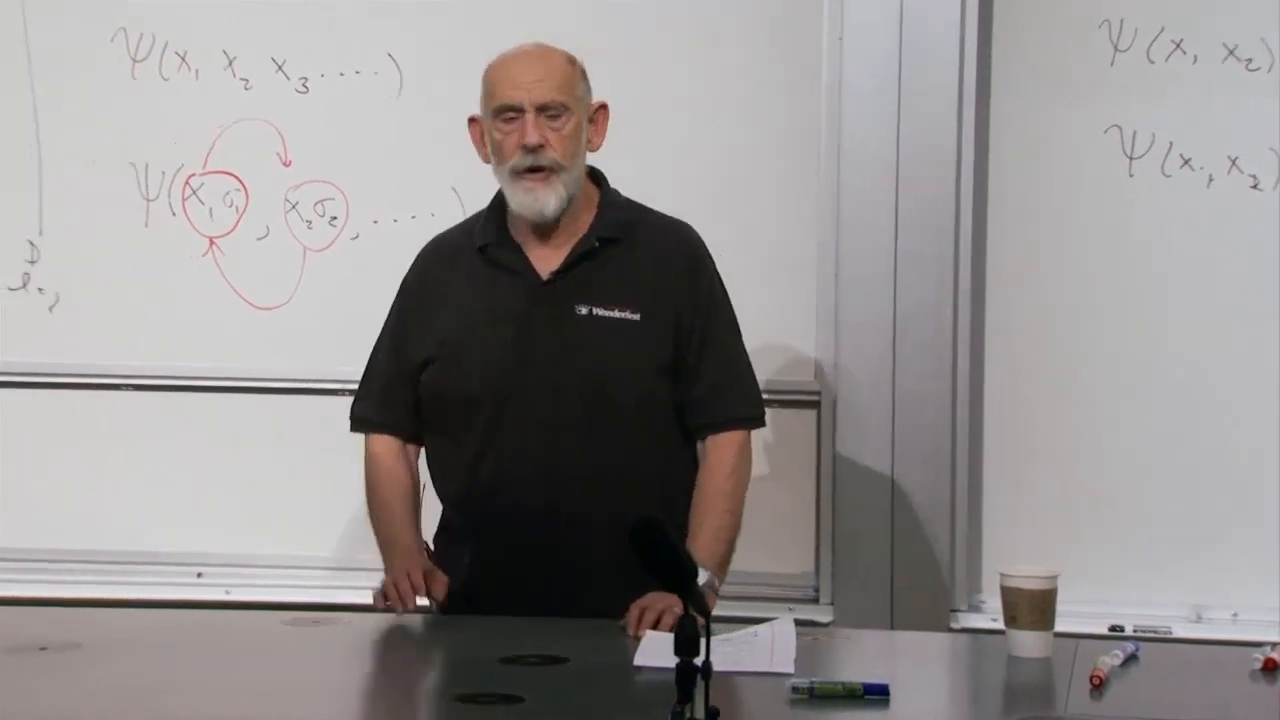
\includegraphics[width=0.9\linewidth]{lecture_05_frame_03.png}
\caption{交換兩個全同粒子時，兩者完整的位置--自旋標記也會互換。玻色子態保持不變，費米子態則改變符號。}
\lectureframe{00:35:25}
\end{figure}

這是線性疊加的兩種不同用法。對單一粒子而言，
\begin{equation}
\alpha\psi_0(x)+\beta\psi_1(x)
\end{equation}
表示兩種可能性的疊加。對兩個粒子而言，
\begin{equation}
\psi_0(x_1)\psi_1(x_2)
\end{equation}
則是在具有兩個粒子座標的空間中的乘積振幅。對稱化或反對稱化會將此乘積與交換後的對應項組合起來。

\begin{classroomqa}
\lecturetimestamp{00:36:13}
\audiencequestion{交換粒子會產生干涉效應嗎？}
\lecturerresponse{會。同一態的費米子振幅為零，可以理解為兩個交換項之間發生了相消干涉。}
\end{classroomqa}

\begin{classroomqa}
\lecturetimestamp{00:37:13}
\audiencequestion{泡利是用同樣的對稱性論證推導出不相容原理的嗎？}
\lecturerresponse{泡利從一項經驗事實出發，找到一個能表述該事實的數學架構。他起初並不是從更基本的理論推導出不相容原理。}
\end{classroomqa}

反對稱性提供了表述經驗性不相容規則的數學架構。

\begin{classroomqa}
\lecturetimestamp{00:39:01}
\audiencequestion{粒子交換干涉和不同可能路徑之間的干涉有關嗎？}
\lecturerresponse{有。一種可能的歷程是兩個粒子不交叉地通過，另一種則是兩者交叉，抵達交換後的位置。玻色子的振幅會相加，費米子的振幅則可能相消。}
\end{classroomqa}

交換帶來第一個負號，旋轉帶來第二個。

\section{第二個負號：旋轉 \texorpdfstring{\(2\pi\)}{2 pi}}

整周旋轉看起來似乎什麼也沒做。轉過角度\(2\pi\)後，每個一般的幾何方向都回到起點。然而，真正必須回到原狀的是機率與期望值。態向量本身可以帶著整體相位回到原狀，正如交換作用也可能使它帶上整體相位。

\begin{classroomqa}
\lecturetimestamp{00:42:12}
\audiencequestion{旋轉是繞哪一條軸進行？生成元是軌道角動量、自旋，還是兩者都有？}
\lecturerresponse{可以選擇一條外部軸；以下選用\(z\)軸。生成元是總角動量，包含軌道角動量與自旋的貢獻。自旋本身不必指向所選的軸。}
\end{classroomqa}

\editorialnote{本段討論的角動量公式採用\(\hbar=1\)，因此\(m\)是\(J_z\)的無量綱本徵值。}

令\(\psi(\theta)\)表示旋轉參數增加至角度\(\theta\)時所得到的態。依照此處採用的慣例，
\begin{equation}
J_z\psi(\theta)
=
-i\frac{\partial}{\partial\theta}\psi(\theta).
\end{equation}
對於具有確定\(J_z\)的態，
\begin{equation}
J_z\psi(\theta)=m\psi(\theta).
\end{equation}
合併這些方程式可得
\begin{equation}
-i\frac{\partial}{\partial\theta}\psi(\theta)
=
m\psi(\theta),
\end{equation}
解為
\begin{equation}
\psi(\theta)=e^{im\theta}\psi(0).
\end{equation}

\(m\)的允許值為整數或半整數。因此
\begin{equation}
\psi(2\pi)
=
\begin{cases}
+\psi(0), & m\in\mathbb Z,\\[4pt]
-\psi(0), & m\in\mathbb Z+\tfrac12.
\end{cases}
\end{equation}
再轉一整圈後，
\begin{equation}
\psi(4\pi)=\psi(0)
\end{equation}
兩種情況都成立。這就是第二個負號：半整數角動量多重態中的態，經過\(2\pi\)旋轉後會改變符號。

這個符號不會改變\(\lvert\psi\rvert^2\)，所以乘在整個態上時無法直接觀察。即便如此，對半整數自旋態而言，\(2\pi\)旋轉所代表的變換並非恆等變換。若能讓這個符號相對於另一個相干振幅產生差異，兩者的不同便可觀測。

\section{\texorpdfstring{\(2\pi\)與\(4\pi\)}{2 pi和4 pi}路徑}

無須進一步推導，就能看出\(2\pi\)與\(4\pi\)之間的差異。一手握住杯子，不放手地轉一整圈。杯子回到原來的朝向，但手臂扭轉了。再繼續轉一圈，手臂便能回到原來的位置，而不必反轉杯子的轉動。

另一種相關的演示，是把球放在盒子裡，再用繩子將球連到盒子。將球轉過\(2\pi\)後，繩子會纏結。在一般的三維空間中，\(4\pi\)轉動所形成的纏結可以解開。關鍵不只是球最後的朝向，而是球在旋轉空間中走過的路徑。

\begin{classroomqa}
\lecturetimestamp{00:54:22}
\audiencequestion{如果球繞同一軸轉兩圈，繩子真的能解開嗎？這需要另一個空間維度嗎？}
\lecturerresponse{\(4\pi\)路徑可以在一般三維空間中解開。時間用來描述運動，不是另一個空間方向。\(2\pi\)路徑無法以這種方式解開，而\(4\pi\)路徑則可以。}
\end{classroomqa}

這些演示呈現了非平凡的\(2\pi\)路徑與可解開的\(4\pi\)路徑之間的差異，無須進一步建立旋轉群的形式理論。

\section{皮帶圖像中的交換與旋轉}

現在可以並列看這兩個負號。交換兩個全同費米子會使其聯合波函數改變符號。將半整數自旋態旋轉\(2\pi\)，也會使其改變符號。皮帶圖像呈現了這兩種操作之間的幾何關聯。

安排皮帶，使下方兩端互相交換。從另一個角度看，同一條皮帶帶有\(2\pi\)的扭轉。若同時進行交換與\(2\pi\)旋轉，扭轉便會消失，留下未扭轉的皮帶。這個組合過程可以連續變形為什麼也不做。\footnote{講座中將交換--旋轉的觀察歸功於David Finkelstein。來源紀錄未指出具體出版物，因此此處只保留講座中的這項歸屬。}

\begin{classroomqa}
\lecturetimestamp{01:01:12}
\audiencequestion{這只是描述皮帶如何嵌入空間，還是也在描述粒子的拓撲？}
\lecturerresponse{皮帶也可以解讀為時空中的粒子歷程。若時間軸朝上，取皮帶的橫截面便會得到類粒子物體。成對的物體被產生，其中一個旋轉\(2\pi\)，接著兩個全同物體互相交換。在這段歷程中，旋轉相位與交換相位彼此抵消。}
\end{classroomqa}

這段歷程清楚呈現了相位的計算方式。起初沒有粒子。在兩個分開的位置各產生一個粒子--反粒子對，因此在中間時刻共有四個粒子。讓其中一個粒子旋轉\(2\pi\)，同時在系統的另一處交換兩個全同粒子。整段歷程可以變形為最基本的歷程：產生一對粒子，之後再將其湮滅。依照此處討論的符號計算，這段平凡歷程不會多出相位。若以\(\eta_{\mathrm{rot}}\)和\(\eta_{\mathrm{ex}}\)表示這兩個符號，講述中的抵消關係可簡潔寫成\footnote{此相位方程式記錄了01：06：50至01：07：18所描述的抵消；講座將這個構造作為啟發性的說明，而非嚴格證明。}
\begin{equation}
\eta_{\mathrm{rot}}\eta_{\mathrm{ex}}=1.
\end{equation}

\begin{classroomqa}
\lecturetimestamp{01:03:34}
\audiencequestion{能不能讓兩個粒子各自移動\(\pi\)，再重新調整它們的方向，藉此將交換和旋轉連結起來？}
\lecturerresponse{這種構造或許反映了相關的數學，但其中使用了兩次各自獨立的\(\pi\)旋轉。此處分析的過程只包含一次\(2\pi\)旋轉，因此兩種論證並不相同。}
\end{classroomqa}

這個論證以粒子類物體能夠被產生和湮滅為前提。若理論中的粒子永恆存在，論證就不會採用這種形式。這也不是自旋--統計定理的標準證明。它的目的，是呈現交換與旋轉的符號彼此吻合的一個拓撲理由。

\section{團塊、鏡像與湮滅}

這個構造也可以用局域場組態來呈現。假設一個或多個場幾乎處處都取真空值，但在某個小區域內具有非零的形狀與結構。這種局域組態稱為團塊。

接著構造第二個組態，使它成為第一個組態適當的鏡像。稱其中一個為粒子，另一個為反粒子。讓兩者靠近，使場組態中彼此對應的部分相遇並相互抵消。在過程中，團塊的某些部分可能已經消失，其他部分仍然存在。繼續變形，剩餘結構也會消失，場便回到真空組態。皮帶上兩個方向相反的扭轉也呈現相同的圖像：將扭轉推到一起，它們便會解開。

這個過程也可以反向進行。空間可以產生一個團塊及其鏡像夥伴。可以產生兩對這樣的物體，將其中一個團塊旋轉\(2\pi\)，交換兩個全同團塊，然後再讓這些物體對湮滅。同樣的交換--旋轉抵消關係也適用於此。這仍是對原構造的啟發式延伸，並非適用於每種局域激發的定理。

\begin{classroomqa}
\lecturetimestamp{01:11:30}
\audiencequestion{有沒有這類團塊場組態的實際例子？}
\lecturerresponse{有。例如，Skyrmion模型描述中的原子核、磁單極子，以及場的其他類粒子激發。}
\end{classroomqa}

鏡像團塊的圖像有助於理解這種推廣。關鍵不在於物體起初是不是基本點粒子，而在於一個類粒子激發及其夥伴能否連續地被產生、彼此靠近並湮滅。這項特性引出旋轉行為與交換行為之間更廣泛的關係。

\begin{classroomqa}
\lecturetimestamp{01:16:12}
\audiencequestion{自旋為二分之一，是否表示態累積的旋轉相位只有通常的一半？}
\lecturerresponse{依照此處的慣例，相位為\(e^{im\theta}\)。對半整數的\(m\)而言，旋轉\(2\pi\)會得到\(-1\)，旋轉\(4\pi\)則會得到\(+1\)。}
\end{classroomqa}

\section{整體符號與零結果實驗}

\(2\pi\)旋轉產生的負號能觀測到嗎？先看一個無法觀測到它的實驗。將電子囚禁在磁場中，緩慢轉動裝置\(2\pi\)，讓電子自旋跟隨磁場，接著將電子釋放到干涉裝置中。再與未進行旋轉、其餘步驟相同的實驗比較。

旋轉使態變為
\begin{equation}
\psi\longmapsto-\psi,
\end{equation}
但負號乘在整個態上，因此所有機率都不變。最終的干涉圖樣不會留下是否曾進行預備旋轉的任何痕跡。這是零結果實驗：共同相位沒有另一個振幅可供干涉。

\begin{classroomqa}
\lecturetimestamp{01:20:01}
\audiencequestion{為什麼磁場必須緩慢旋轉？}
\lecturerresponse{自旋必須持續跟隨旋轉中的磁場。如果磁場轉得太快，自旋就無法持續與磁場保持同步。}
\end{classroomqa}

\section{單一電子的兩個相干分支}

若能讓符號成為相對相位，便可以觀測到它。讓一個電子通過分束器，使它的波函數一部分沿一條路徑前進，另一部分沿另一條路徑前進：
\begin{equation}
\psi(x)=\psi_1(x)+\psi_2(x).
\end{equation}
這是一個電子，不是兩個電子。它處於兩種可能性的相干疊加態。必須清楚區分：這兩個波包不是兩個獨立的粒子。

將兩個波包分別引導到有磁場的區域。在其中一個區域內將磁場旋轉\(2\pi\)，另一個區域則保持不變。對半整數自旋態而言，
\begin{equation}
\psi_1(x)+\psi_2(x)
\longmapsto
\psi_1(x)-\psi_2(x),
\end{equation}
此處將被旋轉分支的標記選為\(2\)。現在符號成為相對的。兩個波包隨後重疊時，原本相加的振幅便改為相減。原本發生相長干涉的位置可能變成相消干涉的位置，甚至形成節點。

\begin{classroomqa}
\lecturetimestamp{01:23:46}
\audiencequestion{只有一個電子，卻有兩個波函數分支；究竟是哪個部分在旋轉？}
\lecturerresponse{電子處於兩個局域化可能性的相干疊加態。一個分支經過旋轉，另一個則沒有。若打開盒子確認電子位於哪個分支，這項測量就會破壞干涉。}
\end{classroomqa}

打開盒子只會看見一個電子，位於其中一個盒子裡。若不進行這項測量，兩個振幅都會保留在態中。重複實驗，探測結果便會逐次累積成干涉圖樣。在相對負號造成的節點位置，不會探測到電子。

\section{磁進動與雙縫干涉}

更實際的示意安排，可以取代極慢的盒子實驗。將相干電子波分成兩條路徑。在其中一條路徑上，讓電子通過磁場區域，且令其自旋初始方向與磁場垂直。接著自旋會進動。調整磁場強度與通過時間，就能讓該分支中的自旋完成一整個\(2\pi\)轉，而另一分支則不經歷這種轉動。\footnote{講座提到一項相關的旋量相位實驗已經進行，並說明其原理；但來源紀錄沒有指出論文或特定裝置。因此，此處僅依講座所述介紹這個構造。}

\begin{classroomqa}
\lecturetimestamp{01:27:05}
\audiencequestion{如何判定單一電子走過哪條路徑？}
\lecturerresponse{無法在不破壞實驗的情況下判定。任何記錄電子所走路徑的測量都會破壞干涉。}
\end{classroomqa}

\begin{classroomqa}
\lecturetimestamp{01:27:50}
\audiencequestion{波函數的分支究竟是什麼？分束器又如何產生兩個分支？}
\lecturerresponse{分支是沿某條路徑局域化的波包。分束器會將入射波分成兩個空間上分離的波包，電場或磁場則可以引導它們沿不同路徑前進。}
\end{classroomqa}

除了磁場區域之外，這就是雙縫實驗。入射電子波分成兩個波包。出射波擴展至共同的探測區域，振幅在此重疊。若沒有相對旋轉，中心處的振幅可能相加。在一條路徑中加入\(2\pi\)自旋旋轉，會使其中一個振幅反號，因而可能讓相同的貢獻互相抵消。

\begin{classroomqa}
\lecturetimestamp{01:30:46}
\audiencequestion{電子穿過不同的管子或狹縫，為什麼還會發生干涉？}
\lecturerresponse{最終的探測不會揭示電子走過哪條路徑。兩個出射波的振幅會在探測器處擴展並重疊。若查看電子走過哪條路徑，干涉就會被破壞。}
\end{classroomqa}

\begin{classroomqa}
\lecturetimestamp{01:33:22}
\audiencequestion{管子或狹縫的直徑必須與電子波長相當嗎？}
\lecturerresponse{若採用字面意義上以繞射為基礎的雙縫設計，開口必須夠小，才能產生所需的擴散。此處描述的是示意裝置，不是實際的設計方案。}
\end{classroomqa}

\begin{classroomqa}
\lecturetimestamp{01:33:44}
\audiencequestion{光子的偏振若也旋轉\(2\pi\)，干涉圖樣會保持不變嗎？}
\lecturerresponse{會。光子具有整數自旋，因此旋轉完整的\(2\pi\)不會引入費米子的負號。}
\end{classroomqa}

\begin{classroomqa}
\lecturetimestamp{01:34:12}
\audiencequestion{實際實驗與理想化版本之間有何細微差異？}
\lecturerresponse{理想的設計讓自旋絕熱地旋轉。在實際情況中，電子會穿過一個磁場區域，自旋進動得較快；不過，測得的相位仍是與旋轉\(2\pi\)一圈相應的相位。}
\end{classroomqa}

緩慢旋轉的設計確保自旋跟隨磁場，不會產生額外運動，藉此凸顯核心概念。進動的設計則透過動力學過程得到相同的相對符號。無論採用哪種設計，兩條路徑都必須變得不可區分，才能形成干涉圖樣。

\begin{classroomqa}
\lecturetimestamp{01:36:15}
\audiencequestion{分束之後，兩個分支必須重新合併嗎？}
\lecturerresponse{是。出射的波包必須彼此重疊，或擴展至共同的探測區域，振幅才能形成干涉圖樣。}
\end{classroomqa}

\begin{classroomqa}
\lecturetimestamp{01:38:12}
\audiencequestion{這個單電子旋轉實驗是泡利不相容原理的結果嗎？}
\lecturerresponse{不是。實驗中只有一個電子。測量的是旋轉時旋量的相位，而不是兩個費米子不能佔據同一個態。}
\end{classroomqa}

\section{交換干涉與相對旋轉}

原則上，同樣的一般方法也能顯示交換符號，不過所提議的裝置更為複雜。先取兩個電子，將它們的聯合波函數分成兩個相干分支。電子仍然只有兩個，不是四個：這一對電子會沿著兩種可能路徑之一演化。在一個分支中交換兩個電子，在另一個分支中則不交換。兩個分支重新合併後，費米子的交換符號會表現為相對相位，並可能改變干涉。

最後的設想直接比較這兩個負號。一個分支取得費米子的交換相位，另一個分支則取得相應的\(2\pi\)旋轉相位。兩者都是\(-1\)，因此相對效應會抵消。\footnote{從01:40:26到01:41:15的錄音清楚呈現了交換相位、\(2\pi\)旋轉相位及兩者的抵消，但根據現有錄音，無法確定旋轉具體如何安排。}講座將此描述為一項思想實驗，並表示據講者所知，這項實驗尚未實際進行。

\begin{classroomqa}
\lecturetimestamp{01:41:34}
\audiencequestion{觀察到交換相位，會對兩個電子的不可區分性構成挑戰嗎？}
\lecturerresponse{不會。量子力學中的不可區分性，比經典意義上的相同性更微妙。即使沒有任何可觀測的標籤能區分粒子，態向量在交換下仍可以改變符號。}
\end{classroomqa}

最後還有一項限定。若將整個孤立世界旋轉\(2\pi\)，只會產生一個共同相位，任何內部實驗都無法測出它。因此，可探測的實驗必須讓一個相干分支相對於另一個分支旋轉。觀察到的不是絕對符號，而是相對符號所造成的干涉。

\chapter{振子、佔據數與第一個量子場}

量子場論是描述幾乎所有已知非重力物理的框架。這並不表示每個問題都能求解。氫原子尚可處理；到了硼這類原子，計算就已經困難得多；至於人體，則遠遠超出任何實際可行的場論計算能力。這個框架或許是基本的，但其中的方程仍然極其難解。

因此，我們將以最基本的方式開始。這個主題有時稱為\emph{二次量子化}，但在建立起所需的數學工具之前，這個名稱還不容易理解。最直接的途徑不是從相對論性場開始，而是從諧振子開始。重點不在彈簧，而在升降算符的代數。當這套代數推廣到許多模式時，升算符就不再只是``將振子提升一個能階''，而是真正具有``產生粒子''的意義。

\section{以代數描述振子}

對單一振子，令\(a^\dagger\)提高激發數，令\(a\)降低激發數。記號\(a_+\)與\(a_-\)等價，但匕首記號預示了場論中使用的語言。基態滿足
\begin{equation}
a|0\rangle=0,
\end{equation}
數算符則為
\begin{equation}
N=a^\dagger a,
\qquad
N|n\rangle=n|n\rangle.
\end{equation}
這兩個階梯算符互為厄米共軛，而其關鍵對易關係是
\begin{equation}
[a,a^\dagger]=1.
\label{eq:l06-single-commutator}
\end{equation}
這個簡單的代數幾乎涵蓋了振子的全部內容。

我們可以從位置與動量的適當線性組合得到\(a\)和\(a^\dagger\)。具體的約定取決於\(x\)、\(p\)、\(m\)和\(\omega\)的正規化；此處有用而不依賴約定的說法是，\(a^\dagger a\)可以重構二次振子的哈密頓量，但會少掉加上的基態能量。因此
\begin{equation}
H=\hbar\omega\left(N+\frac12\right).
\end{equation}
在目前的討論中，我們略去常數項，改用
\begin{equation}
H=\hbar\omega N.
\label{eq:l06-one-oscillator-hamiltonian}
\end{equation}
頻率決定每增加一個激發所需的能量。將\(n\)提高一個激發，需要\(\hbar\omega\)；將\(n\)降低一個激發，則會釋出相同的能量。

\section{多個互相獨立的振子}

現在考慮多個振子，並以\(i\)標記它們。這個標記只是指標，不是虛數單位。模式的數目可以有限，也可以無限。一組互相獨立的彈簧是一種圖像；理想小提琴弦的簡正模式則是另一種。在場論的應用中，重要的是無限多個模式的情形。

獨立性也有算符上的意義。真正屬於互相獨立子系統的算符彼此對易。若不對易，相應的物理量就不能獨立測量，而這些系統也就不是互相獨立的。因此
\begin{align}
[a_i,a_j]&=0, \\
[a_i^\dagger,a_j^\dagger]&=0, \\
[a_i,a_j^\dagger]&=\delta_{ij}.
\label{eq:l06-many-commutators}
\end{align}
當\(i\ne j\)時，屬於這兩個模式的所有量都彼此對易。當\(i=j\)時，最後一行就化為式~\eqref{eq:l06-single-commutator}。

每個振子都有自己的數算符，通常也有自己的頻率：
\begin{equation}
N_i=a_i^\dagger a_i,
\qquad
H=\sum_i\hbar\omega_i N_i.
\label{eq:l06-many-hamiltonian}
\end{equation}
共同本徵態以完整的一組數值標記：
\begin{equation}
|n_1,n_2,n_3,\ldots\rangle,
\qquad n_i=0,1,2,\ldots.
\label{eq:l06-occupation-ket}
\end{equation}
整數\(n_i\)稱為第\(i\)個振子的\emph{佔據數}。此刻這還只是名稱；不久之後，它就會用來計數佔據某個單粒子態的粒子，這個名稱也將名副其實。

所有佔據數都為零的態是
\begin{equation}
|0\rangle\equiv|0,0,0,\ldots\rangle,
\qquad a_i|0\rangle=0\quad\text{for every }i.
\label{eq:l06-oscillator-vacuum}
\end{equation}

\begin{classroomqa}
\lecturetimestamp{00:15:27}
\audiencequestion{無限多個振子是否對應到小提琴弦這類系統的連續模式？}
\lecturerresponse{理想化的弦是如此。真實的弦由原子構成，因此波長短到一定程度時，最終會遇到微觀尺度的截斷。不過，連續模型仍能啟發場論中使用的無限多個模式。}
\end{classroomqa}

\section{階梯係數為何是平方根}

\(a^\dagger\)的作用必須將\(N\)的一個本徵態升至下一個本徵態，但正規化條件仍容許一個係數：
\begin{equation}
a^\dagger|n\rangle=c_n|n+1\rangle.
\label{eq:l06-unknown-coefficient}
\end{equation}

\begin{figure}[htbp]
\centering
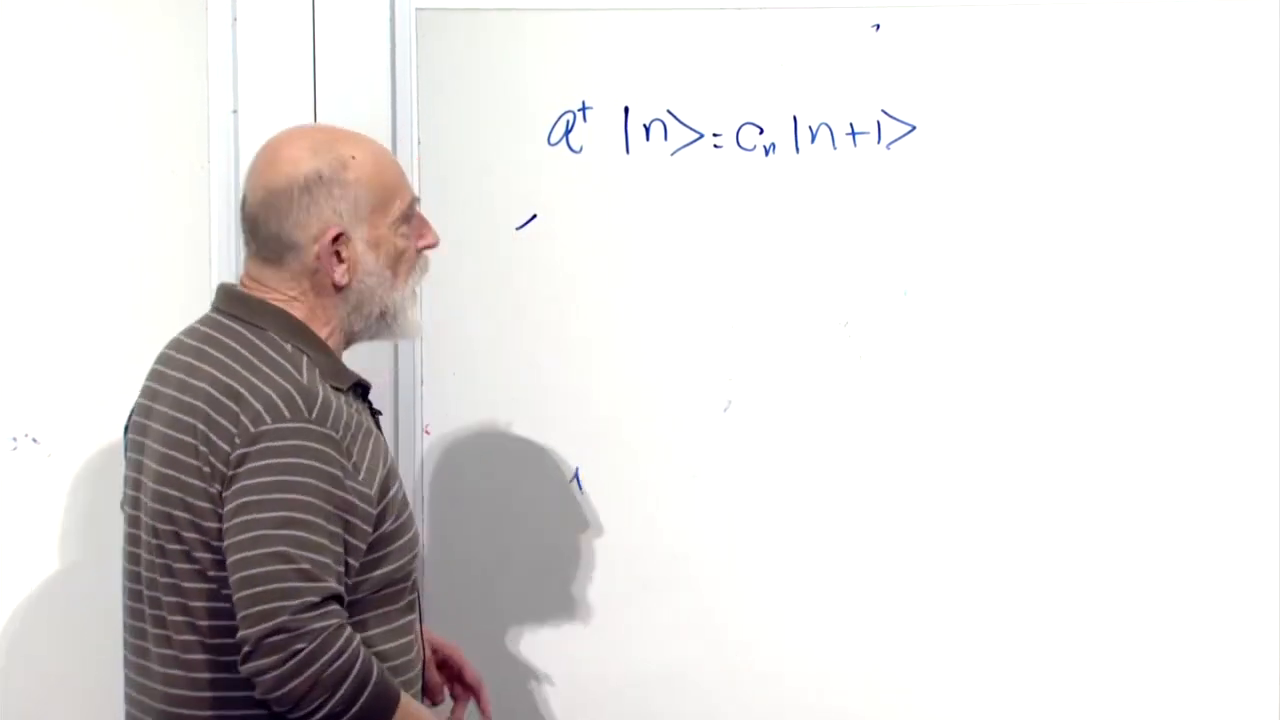
\includegraphics[width=0.9\linewidth]{lecture_06_frame_01.png}
\caption{階梯係數先被引入，之後才推導其正規化。黑板上的方程重現於式~\eqref{eq:l06-unknown-coefficient}。}
\lectureframe{00:19:38}
\end{figure}

選定相位慣例，使\(c_n\)為實數。取厄米共軛可得
\begin{equation}
\langle n|a=c_n\langle n+1|.
\end{equation}
將兩個關係相乘，並利用基底態已正規化的條件，
\begin{align}
c_n^2
&=\langle n|aa^\dagger|n\rangle \\
&=\langle n|(a^\dagger a+1)|n\rangle \\
&=\langle n|(N+1)|n\rangle \\
&=n+1.
\end{align}
因此，
\begin{equation}
a^\dagger|n\rangle=\sqrt{n+1}\,|n+1\rangle.
\label{eq:l06-raising-rule}
\end{equation}

\begin{classroomqa}
\lecturetimestamp{00:22:35}
\audiencequestion{求出\(c_n\)之前，為什麼可以先令\(\langle n+1|n+1\rangle=1\)？}
\lecturerresponse{本徵向量從一開始就選為正規化的基底。它們的正規化並不能決定\(a^\dagger|n\rangle\)的正規化；尚未確定的部分正是係數\(c_n\)。}
\end{classroomqa}

降階規則也可用相同方法推得：
\begin{equation}
a|n\rangle=\sqrt n\,|n-1\rangle.
\label{eq:l06-lowering-rule}
\end{equation}
當\(n=0\)時，係數會自動變為零，因此此規則也包含\(a|0\rangle=0\)。對多個模式而言，算符只會改變自身所對應位置上的佔據數：
\begin{align}
a_i^\dagger|n_1,\ldots,n_i,\ldots\rangle
&=\sqrt{n_i+1}\,|n_1,\ldots,n_i+1,\ldots\rangle, \\
a_i|n_1,\ldots,n_i,\ldots\rangle
&=\sqrt{n_i}\,|n_1,\ldots,n_i-1,\ldots\rangle.
\label{eq:l06-multimode-ladders}
\end{align}
其他項目都不會改變。

\section{波函數不是量子場}

定義場之前，必須先將它與熟悉的波函數區分開來。三個對比有助於理解這個轉變。

第一，單粒子波函數
\begin{equation}
\psi(x)=\langle x|\psi\rangle
\end{equation}
是態向量的一種表示，本身並不是可觀測量。我們測量的是位置、動量、角動量等算符；波函數提供振幅，據此可以計算各種測量結果的機率。

第二，多粒子波函數取決於所有粒子的位置。對兩個粒子，暫且將它們的位置向量稱為\(x\)和\(y\)，則
\begin{equation}
\psi(x,y)=\langle x,y|\psi\rangle.
\end{equation}
這裡的\(x\)和\(y\)代表兩個不同粒子的位置；它們不是同一個位置向量的笛卡兒\(x\)分量與\(y\)分量。對\(N\)個粒子而言，態由下式表示：
\begin{equation}
\psi(x_1,x_2,\ldots,x_N).
\end{equation}

第三，這個波函數描述的是粒子數固定的系統。十五粒子的波函數有十五個位置變數，屬於十五粒子希爾伯特空間。它本身無法描述粒子數從十五變成十四或十六的過程。

量子場則具有相反的特徵：它是算符而非態，依賴單一空間點\(x\)，並作用於涵蓋所有粒子數扇區的態空間。「``一個點''」是指一個可自由變動的位置向量，並不是說\(x\)已被指定為某個數值。

有一項限制在後面會很重要。以下引入的場\(\Psi(x)\)並非厄米算符，因此嚴格來說，它本身不是可觀測量。它的厄米組合才是可觀測量。因此，先前暫時說場可測量，現在要進一步精確說明，而不是撤回：場是算符值函數，而它們的厄米組合代表可測量的物理量。

\begin{classroomqa}
\lecturetimestamp{00:36:52}
\audiencequestion{如果場是位置的函數，位置可以變動嗎？雙粒子波函數中的\(y\)又到哪裡去了？}
\lecturerresponse{點\(x\)會在整個空間中變動。``一個位置''是指算符只有一個空間變數，不是說這個變數固定不動。在\(\psi(x,y)\)中，符號\(x\)和\(y\)分別表示兩個粒子的位置；等價地說，它們是\(x_1\)和\(x_2\)。它們不是場的變數的兩個笛卡兒分量。}
\end{classroomqa}

\begin{classroomqa}
\lecturetimestamp{00:38:15}
\audiencequestion{粒子數固定的波函數描述與場描述如何關聯？它們描述的是不同種類的粒子嗎？}
\lecturerresponse{兩者之間的關聯，正是接下來要建立的核心架構。這些粒子屬於同一種類。本講討論的是玻色子；費米子則需要不同的代數。}
\end{classroomqa}

\section{盒中的單粒子}

暫時回到普通的單粒子量子力學。將一個粒子放進一維盒中。只有一個粒子時，玻色子與費米子的差異無關緊要：沒有第二個相同粒子可用來檢驗交換或排他效應。

令
\begin{equation}
\psi_1(x),\ \psi_2(x),\ \psi_3(x),\ldots
\end{equation}
為能量本徵函數。最低模式是最平滑、且在盒壁處為零的波。下一個模式有一個內部節點；能量更高的模式則振盪得更快。對於寬度為\(L\)的理想無限深方形位能井，一組方便的正規化基底為
\begin{equation}
\psi_i(x)=\sqrt{\frac{2}{L}}\sin\!\left(\frac{i\pi x}{L}\right),
\qquad 0<x<L.
\label{eq:l06-box-basis}
\end{equation}
這個明確的正弦公式是黑板上定性草圖的一種標準表示方式；以下論證只需要一組完備且正交正規的單粒子態。

\begin{figure}[htbp]
\centering
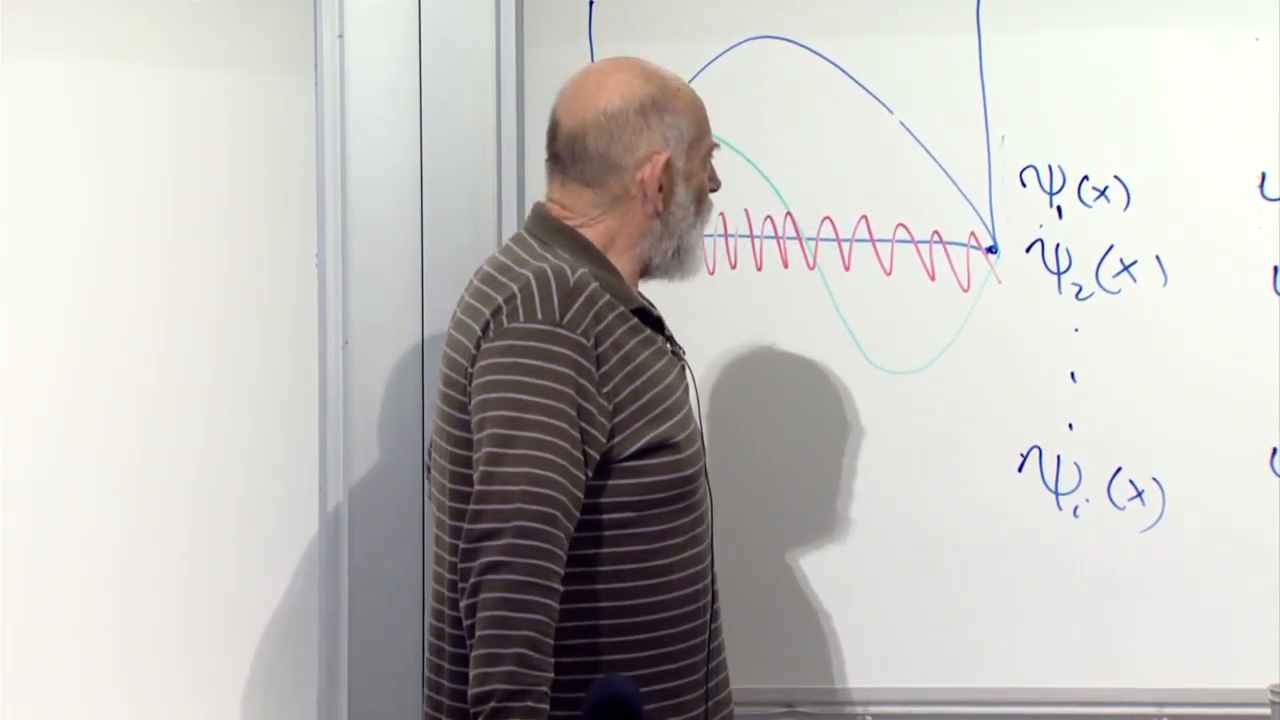
\includegraphics[width=0.9\linewidth]{lecture_06_frame_03.png}
\caption{依能量遞增排列的單粒子盒中模式。第一個模式沒有內部節點，第二個有一個；未畫出的高階模式則振盪得愈來愈快。}
\lectureframe{00:43:10}
\end{figure}

同樣的結構也可以重新繪製，避免受到現場黑板內容遮擋：
\begin{figure}[htbp]
\centering
\begin{tikzpicture}[x=1cm,y=1cm]
  \draw[thick] (0,0) -- (0,3.8);
  \draw[thick] (7,0) -- (7,3.8);
  \draw[gray!55] (0,2.75) -- (7,2.75);
  \draw[gray!55] (0,1.35) -- (7,1.35);
  \draw[blue!75!black,thick,domain=0:7,samples=120]
    plot (\x,{2.75+0.62*sin(180*\x/7)});
  \draw[teal!70!black,thick,domain=0:7,samples=120]
    plot (\x,{1.35+0.55*sin(360*\x/7)});
  \node[right] at (7.15,3.15) {$\psi_1(x)$};
  \node[right] at (7.15,1.70) {$\psi_2(x)$};
  \node at (3.5,0.45) {$\vdots\quad \psi_i(x)$};
\end{tikzpicture}
\caption{盒中模式定性草圖的清晰重繪。為便於辨識，本徵函數在垂直方向上錯開；這不是額外的物理座標。}
\end{figure}

指標\(i\)標記的是單粒子態，不是粒子，也不是節點數。對盒中的基底而言，\(i\)恰好比內部節點數多一。每個態都有能量\(\varepsilon_i\)。依照講課時使用的記號，可以將這個能量寫成\(\hbar\omega_i\)；令\(\hbar=1\)後，也可以簡寫為\(\omega_i\)。

\begin{classroomqa}
\lecturetimestamp{00:39:01}
\audiencequestion{先前假設的獨立性是精確的嗎？指標\(i\)可以標記原子中電子的可能態嗎？}
\lecturerresponse{在獨立模式的架構中，不同模式之間的對易關係是精確的。這個指標可以用來標記原子的單粒子態。不過，若粒子之間有相互作用，簡單的獨立模式哈密頓量就無法完整描述系統。}
\end{classroomqa}

\begin{classroomqa}
\lecturetimestamp{00:40:34}
\audiencequestion{盒中的粒子是玻色子嗎？}
\lecturerresponse{可以是；但只有一個粒子時，統計性質並不重要。只有存在多個相同粒子時，排他效應與交換才有意義。}
\end{classroomqa}

\section{從盒中模式到福克空間}

現在允許盒中有任意數目的相同玻色子。數目為\(n_1\)的粒子可以佔據\(\psi_1\)，數目為\(n_2\)的粒子可以佔據\(\psi_2\)，依此類推。因此，一個基底態為
\begin{equation}
|n_1,n_2,n_3,\ldots\rangle.
\end{equation}
這正是我們用來描述多個振子的記號。兩者在結構上完全對應：每個單粒子態對應一個振子，而振子的激發數等於佔據該態的粒子數。

玻色子在此不可或缺，因為每個\(n_i\)都可以是任意非負整數。費米子的每個單粒子態則只能為空或被一個粒子佔據，不能有兩個粒子同時佔據，因此不能直接沿用一般的振子代數。

現在可以根據算符對佔據數基底的作用來定義這些算符。\(a_i^\dagger\)在單粒子態\(i\)中產生一個粒子；\(a_i\)則移除一個粒子：
\begin{align}
a_i^\dagger|n_1,\ldots,n_i,\ldots\rangle
&=\sqrt{n_i+1}\,|n_1,\ldots,n_i+1,\ldots\rangle, \\
a_i|n_1,\ldots,n_i,\ldots\rangle
&=\sqrt{n_i}\,|n_1,\ldots,n_i-1,\ldots\rangle.
\end{align}
這並非事後才作的類比，而是玻色子產生與湮滅算符在此基底上的定義。由於這組基底張成整個空間，透過線性延伸，這些定義就決定了算符對所有態的作用。

\begin{classroomqa}
\lecturetimestamp{00:47:11}
\audiencequestion{\(n_1,n_2,n_3\)是量子態嗎？}
\lecturerresponse{標記\(1,2,3,\ldots\)指出單粒子態；符號\(n_1,n_2,n_3,\ldots\)表示佔據這些態的粒子數。必須區分態的標記與其佔據數，這是此處主要的記號難點。}
\end{classroomqa}

\subsection{平方根的作用}

因子\(\sqrt{n_i+1}\)不代表額外粒子，也不代表另一種物理過程。它讓算符具有正確的正規化與代數性質。對單一模式而言，
\begin{align}
a a^\dagger|n\rangle
&=a\bigl(\sqrt{n+1}\,|n+1\rangle\bigr) \\
&=(n+1)|n\rangle,
\end{align}
而
\begin{equation}
a^\dagger a|n\rangle=n|n\rangle.
\end{equation}
兩者的差因此是\(|n\rangle\)，符合\([a,a^\dagger]=1\)的要求。非常粗略地說，兩個階梯算符各自的量級約為\(\sqrt n\)，因為它們的乘積會給出量級為\(n\)的數算符。

\begin{classroomqa}
\lecturetimestamp{00:47:52}
\audiencequestion{平方根因子有什麼具體的物理意義？}
\lecturerresponse{它主要是數學上的正規化因子，確保佔據態已正規化、\(a^\dagger a\)的本徵值為\(n\)，並確保階梯算符滿足振子的對易關係。有時候，數學本身就是所需的物理意義。}
\end{classroomqa}

\begin{classroomqa}
\lecturetimestamp{00:52:25}
\audiencequestion{產生算符和湮滅算符是否只根據它們的性質及對基底的作用來定義？}
\lecturerresponse{是的。定義不必建立在更基本的圖像之上。定義的價值要由其推論來檢驗。規定算符對一組完備基底的作用，就能定義它們對所有態的作用，而這些定義也會導出所需的對易關係。}
\end{classroomqa}

\begin{classroomqa}
\lecturetimestamp{00:53:22}
\audiencequestion{為什麼\(a_i\)會讓粒子消失，而不是只把它移到另一個態？}
\lecturerresponse{因為\(a_i\)的定義就是降低態\(i\)的佔據數。有用的問題不是某個定義為什麼成立，而是它為什麼有用。它之所以有用，是因為發射與吸收都需要改變粒子數的算符：輻射發射時會產生光子，吸收時則會湮滅光子。}
\end{classroomqa}

所有佔據數態所張成的空間稱為\emph{福克空間}。其中包含真空、所有單粒子態、所有雙粒子態，依此類推，沒有固定的上限：
\begin{equation}
\mathcal F=\mathcal H_0\oplus\mathcal H_1\oplus\mathcal H_2\oplus\cdots.
\label{eq:l06-fock-space}
\end{equation}
直和記號清楚表明了普通的\(N\)粒子波函數無法表達之處：所有粒子數扇區都屬於同一個態空間。

\begin{classroomqa}
\lecturetimestamp{00:54:56}
\audiencequestion{在佔據數本徵向量上定義算符，就能決定它們對任意向量的作用嗎？接著是否可得振子的對易關係？}
\lecturerresponse{正是如此。佔據數向量構成一組基底，因此透過線性性質，這些定義可延伸至整個福克空間。在這組基底上作用，就能驗證玻色子的對易關係。每個單粒子態都對應一個振子，而振子的佔據數就是該態中的粒子數。}
\end{classroomqa}

\subsection{真空與自由哈密頓量}

福克真空是所有單粒子態都沒有粒子佔據的態：
\begin{equation}
|0\rangle=|0,0,0,\ldots\rangle,
\qquad a_i|0\rangle=0.
\end{equation}
這裡的\emph{基態}一詞可能造成誤解。最低的\emph{單粒子}態是模式\(i=1\)；福克真空中連這個模式也沒有粒子。若有粒子佔據最低模式，\(a_1\)就可以將它移除，使系統回到真空。

\begin{classroomqa}
\lecturetimestamp{00:56:19}
\audiencequestion{用佔據數來說，真空是什麼？最低的單粒子態有粒子佔據嗎？}
\lecturerresponse{真空的所有佔據數都為零，並且會被每個\(a_i\)湮滅。真空中最低的單粒子模式沒有粒子佔據。若有粒子佔據其中，其湮滅算符就能將該粒子移除。}
\end{classroomqa}

對於沒有相互作用的粒子，總能量是各部分能量的總和。若態\(i\)中的一個粒子具有能量\(\hbar\omega_i\)，則
\begin{align}
H
&=\sum_i \hbar\omega_i N_i \\
&=\sum_i \hbar\omega_i a_i^\dagger a_i.
\label{eq:l06-free-fock-hamiltonian}
\end{align}
這個式子有兩種等價的解讀。一種是對振子能量求和，每個單粒子態對應一個振子；另一種是對單粒子能量求和，並將每個能量乘以具有該能量的粒子數。

在場論記號中，\(a_i^\dagger\)通常稱為產生算符，\(a_i\)稱為湮滅算符。較早使用的\(a_+\)與\(a_-\)記號表達的是相同概念。

\section{場出現之前的釐清}

休息後的幾個問題，將新的振子記數方式與普通粒子在振子位能中運動的情形區分開來。

\begin{classroomqa}
\lecturetimestamp{01:06:09}
\audiencequestion{盒中粒子的能階並非等間距，那麼諧振子在哪裡？}
\lecturerresponse{單粒子能量\(\omega_i\)不必等間距。不過，對每個固定模式\(i\)而言，該模式中有零個、一個、兩個或三個互不作用粒子時，能量分別為\(0,\omega_i,2\omega_i,3\omega_i\)。這個佔據數階梯才是這裡所說的振子；它不同於將一個粒子放進諧振子位能中。}
\end{classroomqa}

\begin{classroomqa}
\lecturetimestamp{01:08:38}
\audiencequestion{這個架構與傅立葉分解有關嗎？}
\lecturerresponse{關係非常密切。若單粒子基底由動量模式組成，模式函數就是正弦、餘弦或複指數，而\(a_i\)就是傅立葉係數的量子類比。一般基底不一定由三角函數組成，但展開的邏輯相同。}
\end{classroomqa}

\begin{classroomqa}
\lecturetimestamp{01:09:07}
\audiencequestion{所有粒子的能量都相同嗎？這裡有納入相互作用嗎？}
\lecturerresponse{佔據同一單粒子態的粒子能量相同；處於不同態的粒子，能量通常不同。目前粒子是自由的，也就是彼此不相互作用。相互作用會加入位能項，因此哈密頓量就不再只是式~\eqref{eq:l06-free-fock-hamiltonian}中的可加總和。}
\end{classroomqa}

\begin{classroomqa}
\lecturetimestamp{01:10:26}
\audiencequestion{每個振子中的半個零點能量量子到哪裡去了？}
\lecturerresponse{它是哈密頓量中的加法常數。常數與所有算符對易，因此不會改變海森堡運動方程；一般非重力測量則取決於能量差。這個常數在某些特殊用途上可能很重要，但不影響此處正在建立的架構。}
\end{classroomqa}

自由理論已經是一種威力非凡的記數工具。它不只追蹤許多粒子，也能追蹤粒子態的改變，以及粒子的產生、消失，或總粒子數不同的各種疊加態。這些算符不只是記數符號，因為適當的厄米組合可以測量；不過，記數仍是有用的初步直覺。

\begin{classroomqa}
\lecturetimestamp{01:14:03}
\audiencequestion{場論與量子場論的歷史起源為何？}
\lecturerresponse{簡要來說，這段歷史始於法拉第對電場與磁場的物理圖像，以及馬克士威描述經典場的方程。普朗克研究熱輻射時引入能量量子；愛因斯坦則將量子化與電磁場本身及光量子連結起來。到了1920年代前後，海森堡、泡利，尤其是狄拉克，進一步協助建立現代的算符架構。紫外災難與輻射的量子描述，是早期幾個關鍵問題。這只是一個概略的歷史梗概，並未完整判定各項工作的優先權歸屬。}
\end{classroomqa}

這段歷史也說明了振子為何一再出現。腔中的經典輻射可以分解為簡正模式。將這些模式量子化後，其激發數就成了光子數。佔據模式的數學量子於是成為物理粒子。

\section{玻色場算符}

令\(\{\psi_i(x)\}\)為一組完備且正交正規的單粒子波函數基底。定義
\begin{equation}
\boxed{\Psi(x)=\sum_i a_i\,\psi_i(x)}
\label{eq:l06-field-annihilation}
\end{equation}
以及它的厄米共軛
\begin{equation}
\boxed{\Psi^\dagger(x)=\sum_i a_i^\dagger\,\psi_i^*(x)}.
\label{eq:l06-field-creation}
\end{equation}

\begin{figure}[htbp]
\centering
\includegraphics[width=0.9\linewidth]{lecture_06_frame_04.png}
\caption{湮滅場及其厄米共軛的完整模式展開。排版後的式子~\eqref{eq:l06-field-annihilation}和\eqref{eq:l06-field-creation}保留了相同的算符與複共軛結構。}
\lectureframe{01:25:15}
\end{figure}

對任意固定的位置\(x\)而言，每個\(\psi_i(x)\)都是普通的複數。所有算符成分都在\(a_i\)和\(a_i^\dagger\)之中。隨著\(x\)變動，空間中的每一點都對應不同的算符。這就是\(\Psi\)作為算符值函數的確切含義。

若基底函數是平面波，式~\eqref{eq:l06-field-annihilation}和\eqref{eq:l06-field-creation}就是量子版的傅立葉展開：經典傅立葉係數在此變成了算符。在盒中，基底也可以採用式~\eqref{eq:l06-box-basis}中的正弦函數。任何完備且正交正規的單粒子基底都適用。

\(\Psi\)和\(\Psi^\dagger\)都不是厄米算符。可觀測場可以由厄米組合構成，例如
\begin{equation}
\Psi(x)+\Psi^\dagger(x),
\qquad
i\bigl(\Psi^\dagger(x)-\Psi(x)\bigr),
\end{equation}
稍後也會以\(\Psi^\dagger(x)\Psi(x)\)這類乘積構造可觀測密度。目前首先要了解的是這兩個基本場的作用。

\begin{classroomqa}
\lecturetimestamp{01:23:14}
\audiencequestion{右邊的模式函數是普通波函數，左邊怎麼會是算符？}
\lecturerresponse{選定\(x\)後，函數\(\psi_i(x)\)就是數值。因子\(a_i\)是算符。數乘上算符仍是算符，因此總和也是算符。改變\(x\)，就會得到一整族算符。}
\end{classroomqa}

\section{場的作用}

湮滅場會立刻湮滅真空：
\begin{equation}
\Psi(x)|0\rangle
=\sum_i\psi_i(x)a_i|0\rangle
=0.
\label{eq:l06-field-kills-vacuum}
\end{equation}
產生場的作用則更能說明問題。

令\(|i\rangle\)表示波函數為
\begin{equation}
\langle x|i\rangle=\psi_i(x).
\end{equation}
的單粒子態。單粒子基底的完備性給出
\begin{equation}
\sum_i|i\rangle\langle i|=1.
\label{eq:l06-completeness}
\end{equation}
將此恆等式作用於位置本徵態：
\begin{align}
|x\rangle
&=\sum_i|i\rangle\langle i|x\rangle \\
&=\sum_i\psi_i^*(x)|i\rangle.
\label{eq:l06-position-expansion}
\end{align}
在福克空間的記號中，單粒子模式態為
\begin{equation}
|i\rangle=a_i^\dagger|0\rangle.
\end{equation}
將其代入式~\eqref{eq:l06-position-expansion}，可得
\begin{align}
|x\rangle
&=\sum_i\psi_i^*(x)a_i^\dagger|0\rangle \\
&=\Psi^\dagger(x)|0\rangle.
\label{eq:l06-local-creation}
\end{align}
因此，\(\Psi^\dagger(x)\)會在\(x\)處產生一個局域化粒子，而\(\Psi(x)\)則會在該處湮滅一個粒子。位置本徵態具有狄拉克 {\proseunicodefont δ} 函數的局域化性質，是一種廣義且不可正規化的態；實際的局域化粒子則須以可正規化的波包將場加權積分而得。\editorialnote{本講採用理想的位置本徵態描述。波包這項補充說明交代了標準的數學意義，並未改變論證。}

\begin{classroomqa}
\lecturetimestamp{01:36:26}
\audiencequestion{如何指定所產生粒子種類的資訊？在\(x\)處的態是狄拉克 {\proseunicodefont δ} 函數局域化的嗎？}
\lecturerresponse{每種粒子都對應一個獨立的場，因此粒子的種類由所使用的場決定。變數\(x\)指定粒子在哪裡產生。在理想的位置基底中，所產生的態具有狄拉克 {\proseunicodefont δ} 函數的局域化性質。}
\end{classroomqa}

玻色子種類的例子包括光子、重力子、希格斯玻色子與膠子，不過實際的場也帶有內部指標。即使是光子也需要偏振標記。簡化的純量場記號省略這些額外標記，讓粒子產生的原理更清楚。

\subsection{真空不是零向量}

方程
\begin{equation}
\Psi(x)|0\rangle=0
\end{equation}
中以零表示的兩個對象截然不同。右矢\(|0\rangle\)是真空，是一個正規化的物理態，滿足
\begin{equation}
\langle0|0\rangle=1.
\end{equation}
右側的結果則是零向量。它的範數為零，無法正規化，也不代表物理態。

做加法時，兩者的差異就很明顯。將零向量加到單粒子態上，結果不變；將真空加到單粒子態上，則會得到不同粒子數扇區的真正疊加態。使用正規化係數時，
\begin{equation}
|\chi\rangle=\frac{1}{\sqrt2}\bigl(|0\rangle+|1\rangle\bigr)
\end{equation}
零粒子與一個粒子的機率相同。這個態不同於\(|1\rangle\)。

\begin{classroomqa}
\lecturetimestamp{01:37:23}
\audiencequestion{如果在\(x\)處沒有粒子，\(\Psi(x)\)是否就什麼也不做？結果為零又代表什麼？}
\lecturerresponse{它不會返回原來的態，而是返回零向量。真空是描述空間為空的歸一化態；零向量的長度為零，且不描述任何物理態。任何算符作用在零向量上，都會返回零向量。}
\end{classroomqa}

\begin{classroomqa}
\lecturetimestamp{01:39:00}
\audiencequestion{如果把真空而非零向量加到單粒子態上，會得到什麼？}
\lecturerresponse{得到的是一個包含不同粒子數振幅的疊加態。相較之下，加上零向量不會改變單粒子態。符號\(|0\rangle\)表示零佔據數，並不代表零向量。}
\end{classroomqa}

\begin{classroomqa}
\lecturetimestamp{01:41:56}
\audiencequestion{在場的展開式中，模式函數與其產生或湮滅算符的次序重要嗎？模式函數可以是複數嗎？}
\lecturerresponse{模式函數是普通數，因此與所有算符對易，次序並不重要。一般而言，模式函數可以是複數；所選基底是實數還是複數，取決於單粒子Schr\"odinger問題。}
\end{classroomqa}

\subsection{兩粒子與玻色對稱性的形成}

要在\(x\)處產生一個粒子，並在\(y\)處產生另一個粒子，只要作用兩次：
\begin{equation}
|x,y\rangle
=\Psi^\dagger(y)\Psi^\dagger(x)|0\rangle.
\label{eq:l06-two-particle-state}
\end{equation}
這兩個位置可以重合，也可以不同。由於底層的產生算符彼此對易，
\begin{align}
[\Psi^\dagger(x),\Psi^\dagger(y)]
&=\sum_{i,j}\psi_i^*(x)\psi_j^*(y)
[a_i^\dagger,a_j^\dagger] \\
&=0.
\end{align}
因此可得
\begin{equation}
\Psi^\dagger(y)\Psi^\dagger(x)|0\rangle
=\Psi^\dagger(x)\Psi^\dagger(y)|0\rangle.
\label{eq:l06-boson-exchange}
\end{equation}
交換兩個粒子的次序不會造成任何改變，這正是玻色交換對稱性。因此，我們也可以從振子代數出發，\emph{推導出}由彼此對易的產生算符所構造的粒子是玻色子。費米子則需要使用反對易算符。

\begin{classroomqa}
\lecturetimestamp{01:42:37}
\audiencequestion{如何在單粒子態中加入第二個粒子？}
\lecturerresponse{再作用一個產生場即可。若要在\(y\)處加入粒子，就讓\(\Psi^\dagger(y)\)作用在\(\Psi^\dagger(x)\)的左側。所得結果就是方程式~\eqref{eq:l06-two-particle-state}中的兩粒子態。}
\end{classroomqa}

\begin{classroomqa}
\lecturetimestamp{01:46:04}
\audiencequestion{兩個產生場彼此對易，是否就完全等同於將兩粒子態對稱化？}
\lecturerresponse{是。這使得一個粒子在\(x\)處、另一個在\(y\)處的態，與交換標記後得到的態完全相同。這就是全同玻色子的定義性交換性質。}
\end{classroomqa}

\begin{classroomqa}
\lecturetimestamp{01:46:32}
\audiencequestion{這是否表示\(x\)和\(y\)處的粒子必須是同一種類的玻色子？}
\lecturerresponse{是。\(x\)和\(y\)是位置，而一個場描述一種粒子。不同種類的粒子，以及例如光子的兩種偏振等額外標記，都需要不同的場分量。}
\end{classroomqa}

\section{可變粒子數為何重要}

如果一個問題永遠都恰好包含三十七個粒子，那麼場的語言就只是可有可無的記帳方式。場論真正的威力，在粒子可以被發射和吸收時才會顯現；尤其當粒子數本身是量子變數時，更是如此。Fock 空間允許如下形式的態：
\begin{equation}
|\Phi\rangle
=c_0|0\rangle+c_1|1\rangle+c_2|2\rangle+\cdots,
\qquad
\sum_{n=0}^{\infty}|c_n|^2=1.
\end{equation}
雷射場是一個重要例子：它通常不是具有確定光子數的態，而是許多粒子數扇區的疊加。

粒子與場之間的橋樑如今已清楚呈現。模式算符計數能量本徵態中的粒子，並改變粒子數；場則將這些算符與一組完備波函數結合，使粒子能在指定位置被產生或移除。諧振子的代數已成為玻色量子場的基本語言。

\chapter{從粒子到簡單量子場}

讓我們再從稍有不同的角度，建構這個簡單的量子場。進入量子場論有兩條路：我們可以從粒子出發，探究為什麼場是描述粒子的自然語言；也可以從波場出發，探究為什麼它的激發以量子的形式出現。兩條路都很有用。這裡我們走第一條。

普通量子力學可以描述一個粒子、兩個粒子，或任何其他固定粒子數。自然界並不受這項限制。每當燈發射或吸收輻射，房間裡的光子數就會改變。不穩定粒子會衰變。例如在 {\proseunicodefont β} 衰變中，
\begin{equation}
n\longrightarrow p+e^-+\bar{\nu}_e,
\end{equation}
因此，數種粒子的數量會同時改變。我們需要一套足夠廣泛的量子力學，能容納所有可能的佔據數，並且最終能描述佔據數彼此轉換的過程。

目前我們先大幅簡化問題：只有一種非相對論性粒子。我們先擴大它的態空間，使其能容納任意粒子數，之後再討論更多粒子種類、相對論、散射與衰變。數學本身並不特別困難，但觀點的轉變很抽象。值得放慢腳步，免得記號掩蓋了想法。

\section{從單粒子出發}

先從一個處於態 \(|\psi\rangle\) 的單粒子開始。它在位置空間中的波函數為
\begin{equation}
\psi(x)=\langle x|\psi\rangle.
\label{eq:l07-wavefunction}
\end{equation}
這個小寫的 \(\psi\) 是普通的複值函數。它還不是量子場，也不是作用於多粒子態空間的算符。

玻恩定則指出，
\begin{equation}
\rho_\psi(x)=|\psi(x)|^2=\psi^*(x)\psi(x)
\label{eq:l07-born-density}
\end{equation}
是粒子出現在 \(x\) 處的機率密度。對於歸一化的態，
\begin{equation}
\int dx\,\psi^*(x)\psi(x)=1.
\label{eq:l07-one-particle-normalization}
\end{equation}
右側等於總機率。由於這裡恰好只有一個粒子，總機率也恰好等於粒子數。這個巧合雖然在此無足為奇，稍後卻會成為有用的線索。

\begin{classroomqa}
\lecturetimestamp{00:09:13}
\audiencequestion{為什麼機率密度必須寫成 \(\psi^*(x)\psi(x)\) 的形式？}
\lecturerresponse{這就是玻恩定則，是量子力學的公設之一。位置測量結果為 \(x\) 的振幅是 \(\langle x|\psi\rangle\)；機率密度則是振幅的絕對值平方。這不是從後文的場構造推導出來的。}
\end{classroomqa}

\section{模式、正交性與完備性}

單粒子希爾伯特空間有許多有用的基底。位置本徵態構成一組基底；任何厄米算符的本徵態也構成另一組基底，但簡併與連續譜的情況須按通常方式處理。由於能量很快就會派上用場，我們選取一組完備且正交歸一的單粒子能量本徵態：
\begin{equation}
|1\rangle,\ |2\rangle,\ldots,
\qquad
\psi_i(x)=\langle x|i\rangle.
\end{equation}

盒中粒子的例子讓指標 \(i\) 變得具體。基態波函數沒有內部節點，下一個態有一個節點，更高能態的振盪則愈來愈快。對理想的無限深方形位能井而言，這些波函數本質上就是正弦波。

\begin{figure}[htbp]
\centering
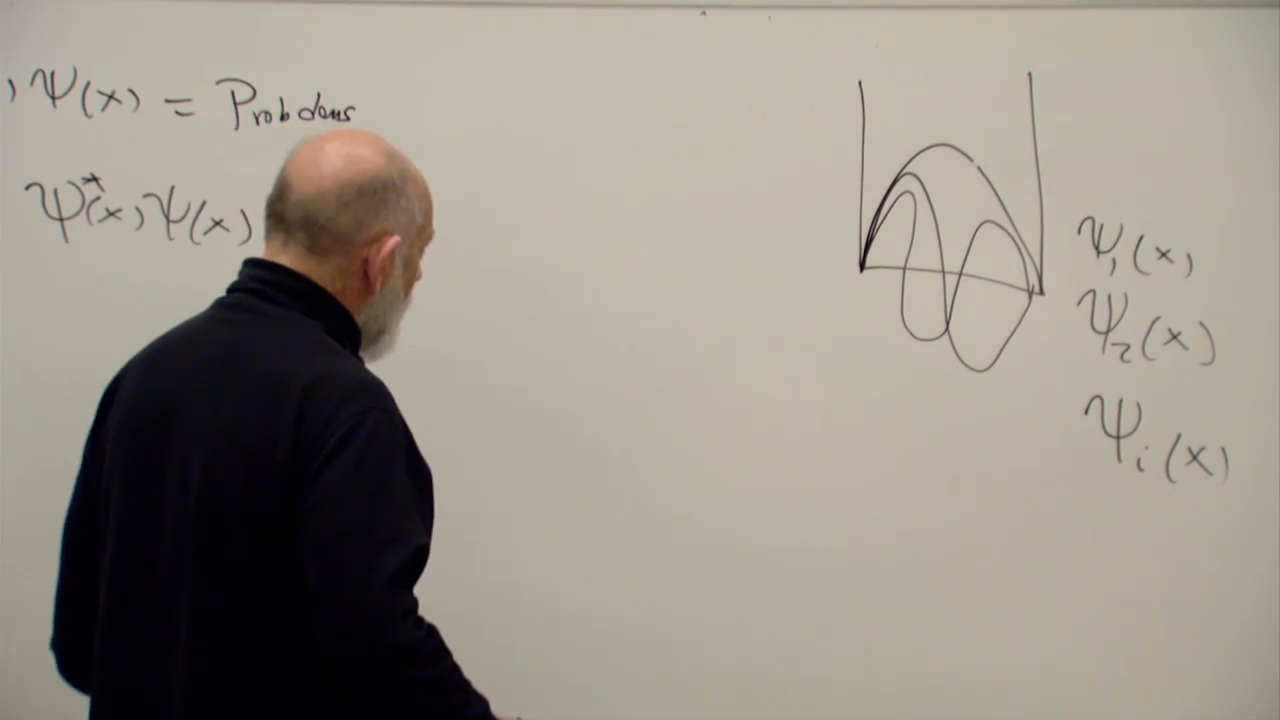
\includegraphics[width=0.94\linewidth]{lecture_07_frame_01.png}
\caption{課堂黑板上的盒中模式。左側殘留的內容是單粒子的玻恩機率密度與歸一化；右側的位能井則畫出 \(\psi_1(x)\)、\(\psi_2(x)\)，以及一般標記 \(\psi_i(x)\)。}
\lectureframe{00:08:25}
\end{figure}

即使黑板上的內容有所遮擋，仍可分辨出相同的模式結構：
\begin{figure}[htbp]
\centering
\begin{tikzpicture}[x=1cm,y=1cm]
  \draw[thick] (0,0) -- (0,4.0);
  \draw[thick] (7,0) -- (7,4.0);
  \draw[gray!55] (0,2.85) -- (7,2.85);
  \draw[gray!55] (0,1.35) -- (7,1.35);
  \draw[blue!75!black,thick,domain=0:7,samples=120]
    plot (\x,{2.85+0.62*sin(180*\x/7)});
  \draw[teal!70!black,thick,domain=0:7,samples=120]
    plot (\x,{1.35+0.55*sin(360*\x/7)});
  \node[right] at (7.15,3.20) {$\psi_1(x)$};
  \node[right] at (7.15,1.70) {$\psi_2(x)$};
  \node at (3.5,0.38) {$\vdots\quad\psi_i(x)$};
\end{tikzpicture}
\caption{盒中模式示意圖的清晰重繪。兩個波函數在垂直方向上的位移只是為了方便展示。}
\end{figure}

正交歸一關係為
\begin{equation}
\int dx\,\psi_i^*(x)\psi_j(x)=\delta_{ij}.
\label{eq:l07-orthonormality}
\end{equation}
若 \(i=j\)，態便已歸一化，積分值為一；若 \(i\ne j\)，兩個態便彼此正交，積分值為零。

同樣重要的完備性關係是
\begin{equation}
\sum_i |i\rangle\langle i|=\mathbf 1.
\label{eq:l07-resolution}
\end{equation}
每個 \(|i\rangle\langle i|\) 都投影到一個基底方向；對完備基底求和則得到恆等算符。它作用於任意向量時，只是先將向量分解成各分量，再將分量合併還原。

現在將式~\eqref{eq:l07-resolution}夾在兩個位置態之間：
\begin{align}
\langle y|x\rangle
&=\sum_i\langle y|i\rangle\langle i|x\rangle \\
&=\sum_i\psi_i(y)\psi_i^*(x) \\
&=\delta(y-x).
\label{eq:l07-position-completeness}
\end{align}
複共軛星號應加在左矢右矢順序為 \(\langle i|x\rangle\) 的那一項上。交換 \(x\) 和 \(y\) 的位置，便會得到複共軛但等價的形式。因此，每一組完備的正交歸一基底都能表示 {\proseunicodefont δ} 函數。正弦函數、餘弦函數、振子波函數與能量本徵函數都能完成同樣的工作。

\begin{classroomqa}
\lecturetimestamp{00:13:43}
\audiencequestion{完備性求和中的第二個波函數是否應該帶有複共軛？}
\lecturerresponse{是的。依照 \(\langle y|i\rangle\langle i|x\rangle\) 的順序，兩個因子是 \(\psi_i(y)\psi_i^*(x)\)。保留明確的左矢右矢順序，就不必靠猜測來決定星號的位置，也能避免放錯。}
\end{classroomqa}

這就是我們需要的單粒子數學。現在來改變態空間。

\section{作為擴大態空間的福克空間}

對許多全同粒子而言，一組方便的基底會記錄每個單粒子模式中有多少粒子：
\begin{equation}
|n_1,n_2,n_3,\ldots\rangle.
\label{eq:l07-fock-basis}
\end{equation}
整數 \(n_i\) 是模式 \(i\) 的佔據數。這個右矢不是用花俏記號寫成的單粒子態；它屬於一個更大的希爾伯特空間，其中包含零粒子扇區、所有單粒子態、所有雙粒子態，依此類推。這個更大的空間稱為福克空間。

若要改變佔據數，便為每個模式引入一個產生算符和一個湮滅算符：
\begin{equation}
a_i^\dagger,\qquad a_i.
\end{equation}
前者在模式 \(i\) 中增加一個粒子，後者則移除一個粒子。在這裡，諧振子的語言只是記錄佔據數的工具：不一定真有一根彈簧在振動。諧振子代數恰好提供了升高與降低佔據數所需的機制。

模式數算符為
\begin{equation}
\begin{aligned}
N_i&=a_i^\dagger a_i,\\
N_i|n_1,\ldots,n_i,\ldots\rangle
&=n_i|n_1,\ldots,n_i,\ldots\rangle.
\end{aligned}
\end{equation}
真空態為
\begin{equation}
|0\rangle\equiv|0,0,0,\ldots\rangle,
\qquad
a_i|0\rangle=0
\quad\text{for every }i.
\label{eq:l07-vacuum}
\end{equation}
因此，模式 \(i\) 中的單粒子態為
\begin{equation}
|i\rangle=a_i^\dagger|0\rangle.
\label{eq:l07-mode-created}
\end{equation}
同一個符號 \(|i\rangle\) 現在既可以表示單粒子基底向量，也可以表示嵌入福克空間單粒子扇區中的該向量。這項嵌入由式~\eqref{eq:l07-mode-created}給出；我們正在討論哪個空間，則由上下文決定。

\section{將各模式組合成場}

定義湮滅場與產生場如下：
\begin{equation}
\Psi(x)=\sum_i \psi_i(x)a_i,
\qquad
\Psi^\dagger(x)=\sum_i \psi_i^*(x)a_i^\dagger.
\label{eq:l07-field-expansion}
\end{equation}
大小寫很重要。小寫函數 \(\psi_i(x)\) 是複數；大寫的 \(\Psi(x)\) 則是作用於福克空間的算符。對每個空間位置 \(x\)，式~\eqref{eq:l07-field-expansion}都給出一個不同的模式算符線性組合。這就是「位置的算符值函數」的意思。

對自由粒子，模式函數可以是平面波 \(e^{ikx}\)。此時式~\eqref{eq:l07-field-expansion}便是傅立葉展開，只是傅立葉係數由算符而非數值構成。舊有術語把普通複數稱為 \(c\) 數，把量子算符稱為 \(q\) 數。模式函數是 \(c\) 數，與所有對象都對易；\(a_i\) 和 \(a_i^\dagger\) 則具有算符的性質。

\(\Psi\) 和 \(\Psi^\dagger\) 都不是厄米算符；它們的厄米共軛互為對方。以下兩個組合
\begin{equation}
\Psi+\Psi^\dagger,
\qquad
i(\Psi^\dagger-\Psi)
\label{eq:l07-hermitian-combinations}
\end{equation}
則是厄米算符，可以代表可觀測量。不過目前而言，場最有用之處，是能在局部產生、湮滅並計數粒子。

\begin{classroomqa}
\lecturetimestamp{00:21:05}
\audiencequestion{算符依賴於 \(x\) 是什麼意思？}
\lecturerresponse{意思是，\(x\) 的每個取值都對應一個不同的算符。空間依賴性來自普通的模式函數，而每個由此得到的線性組合都作用於同一個福克空間。}
\end{classroomqa}

\section{產生場的作用}

要知道定義有何用處，就得看它如何作用。從單粒子扇區中的位置本徵態出發，並插入單位算符的完備關係：
\begin{align}
|x\rangle
&=\sum_i |i\rangle\langle i|x\rangle \\
&=\sum_i a_i^\dagger|0\rangle\,\psi_i^*(x) \\
&=\Psi^\dagger(x)|0\rangle.
\label{eq:l07-local-creation}
\end{align}
因此，\(a_i^\dagger\)會在確定的模式 \(i\) 中產生一個粒子；\(\Psi^\dagger(x)\)則會在位置 \(x\) 產生一個局域化的粒子。在理想化的位置基底中，這種局域化是以分布的意義成立；實際製備會使用狹窄的波包，但代數上的意義相同。

\begin{classroomqa}
\lecturetimestamp{00:24:48}
\audiencequestion{\(\sum_i|i\rangle\langle i|\)是投影算符嗎？}
\lecturerresponse{每一項都是投影到一個基底態的投影算符。對完整基底求和得到的就是恆等算符，稱為單位算符的完備關係。插入這個關係不會改變任何態，卻能顯示該態在所選基底中的各個分量。}
\end{classroomqa}

式~\eqref{eq:l07-local-creation}直接揭示了場的粒子意義。我們不只是替抽象算符加上空間標記，而是構造出在該空間位置產生粒子的操作。

\begin{classroomqa}
\lecturetimestamp{00:28:20}
\audiencequestion{位置空間中的產生場應該標上星號還是匕首？}
\lecturerresponse{算符的厄米共軛要用匕首符號。星號表示普通波函數 \(\psi_i(x)\) 的複共軛；匕首符號則標在 \(a_i^\dagger\) 和 \(\Psi^\dagger(x)\) 上。}
\end{classroomqa}

\begin{classroomqa}
\lecturetimestamp{00:28:36}
\audiencequestion{在模式展開式中，可以把產生算符移過波函數嗎？}
\lecturerresponse{可以。\(\psi_i(x)\) 是 \(c\) 數，因此與所有算符都對易。只有在調換 \(a_i\) 和 \(a_j^\dagger\) 這類不對易算符的順序時，才需要小心。}
\end{classroomqa}

\section{從機率密度到粒子密度}

現在來看看這個場。首先自然會考慮
\begin{equation}
\int dx\,\Psi^\dagger(x)\Psi(x).
\end{equation}
它看起來像單粒子的歸一化積分，但現在其中的因子是算符。代入模式展開式，並保持算符的順序不變：
\begin{align}
\int dx\,\Psi^\dagger(x)\Psi(x)
&=\int dx
\left(\sum_i a_i^\dagger\psi_i^*(x)\right)\\
&\qquad\times\left(\sum_j a_j\psi_j(x)\right) \\
&=\sum_{i,j}a_i^\dagger a_j
\int dx\,\psi_i^*(x)\psi_j(x) \\
&=\sum_{i,j}a_i^\dagger a_j\,\delta_{ij} \\
&=\sum_i a_i^\dagger a_i.
\label{eq:l07-number-derivation}
\end{align}
因此，總粒子數算符為
\begin{equation}
N=\sum_i N_i
=\int dx\,\Psi^\dagger(x)\Psi(x).
\label{eq:l07-total-number}
\end{equation}
對於這裡討論的態，高能模式上的佔據數會逐漸趨近於零，因此即使可能的模式無窮多，粒子總數通常仍有限。

被積分項是局部粒子密度算符：
\begin{equation}
n(x)=\Psi^\dagger(x)\Psi(x).
\label{eq:l07-density}
\end{equation}
嚴格來說，密度不能在數學上的單一點測量。對於小區域 \(R\)，實際測量的是
\begin{equation}
N_R=\int_R dx\,n(x),
\label{eq:l07-regional-number}
\end{equation}
也就是該區域內的粒子數。和其他量子可觀測量一樣，\(N_R\) 在任意態中不一定有確定值。重複製備同一狀態，測量結果可能不同。

\begin{classroomqa}
\lecturetimestamp{00:36:27}
\audiencequestion{\(\Psi^\dagger(x)\Psi(x)\)是多粒子機率密度嗎？}
\lecturerresponse{它直接表示的是粒子密度。多粒子機率振幅一般取決於所有粒子的座標；而這個局部雙線性算符若在某個小區域上積分，計算的則是該區域內的粒子數。}
\end{classroomqa}

\begin{classroomqa}
\lecturetimestamp{00:38:28}
\audiencequestion{算符 \(a_i\) 和 \(a_i^\dagger\) 只作用於態向量，不作用於單粒子波函數嗎？}
\lecturerresponse{是的。它們作用於福克空間中的態，例如 \(|n_1,n_2,\ldots\rangle\)。乘在這些算符前面的單粒子模式函數是普通數值，並非這些升降算符作用的對象。}
\end{classroomqa}

佔據數態構成一組基底，卻不是一般態的唯一形式。它們可以疊加；例如，總粒子數相同，但粒子在不同模式間分布方式不同的態也可以疊加。對光子這類中性粒子而言，不同總粒子數的態也可以疊加。式~\eqref{eq:l07-regional-number}中的算符在這些態中都具有相同的操作意義。

\begin{classroomqa}
\lecturetimestamp{00:40:01}
\audiencequestion{若以總粒子數除粒子密度，是否就得到粒子出現在 \(x\) 處的機率密度？}
\lecturerresponse{在固定 \(N\) 且粒子數很大的情況下，\(N_R/N\) 是相對頻率，通常能很好地反映單粒子機率。但這並不是一條算符恆等式，不能把單次測量結果等同於機率。在獨立粒子的圖像中，測得的計數會有漲落，典型幅度約為 \(\sqrt N\)；偶爾一次測量也可能與機率相差很大，雖然這種情況不常見。}
\end{classroomqa}

\begin{classroomqa}
\lecturetimestamp{00:42:25}
\audiencequestion{若將一電子態與零電子態疊加，電荷守恆會如何？}
\lecturerresponse{這不是固定電荷封閉扇區中所使用的那種疊加。可以疊加總電荷相同、但粒子分布不同的態。光子不帶電，因此不同光子數扇區的疊加不會造成這個問題。電子數與正電子數也可以同時改變，而淨電荷仍保持不變。}
\end{classroomqa}

\section{獨立粒子的能量}

接下來要看的是能量。先考慮彼此不交互作用的粒子。在稀薄系統中，這通常是很好的近似。原則上，光子也會透過高階過程彼此交互作用；但普通實驗室中的輻射足夠稀薄，因此獨立粒子的描述非常準確。

令 \(\omega_i\) 表示模式 \(i\) 中單一粒子的能量，其中 \(\hbar=1\)。模式就是一個單粒子態。於是總哈密頓量為
\begin{equation}
H=\sum_i\omega_i N_i
=\sum_i\omega_i a_i^\dagger a_i.
\label{eq:l07-mode-hamiltonian}
\end{equation}
每個被佔據的模式中，每一個粒子都各自貢獻一次其單粒子能量。

\begin{classroomqa}
\lecturetimestamp{00:48:16}
\audiencequestion{\(\omega_i\)是位置的函數嗎？}
\lecturerresponse{不是。它是與模式 \(i\) 對應的能量本徵值。函數 \(\psi_i(x)\) 依賴位置；\(\omega_i\) 則取決於選中了哪個能階。}
\end{classroomqa}

數值 \(\omega_i\) 由單粒子定態薛丁格方程決定。定義
\begin{equation}
h=-\frac{\nabla^2}{2m}+V(x).
\label{eq:l07-one-particle-h}
\end{equation}
於是
\begin{equation}
h\psi_i(x)=\omega_i\psi_i(x).
\label{eq:l07-schrodinger-eigenvalue}
\end{equation}
在一維中，動量算符是 \(p=-i\partial_x\)，而 \(p^2/(2m)\) 就是 \(-\partial_x^2/(2m)\)。在三維中，三個二階導數合併為 \(-\nabla^2/(2m)\)。

\begin{figure}[htbp]
\centering
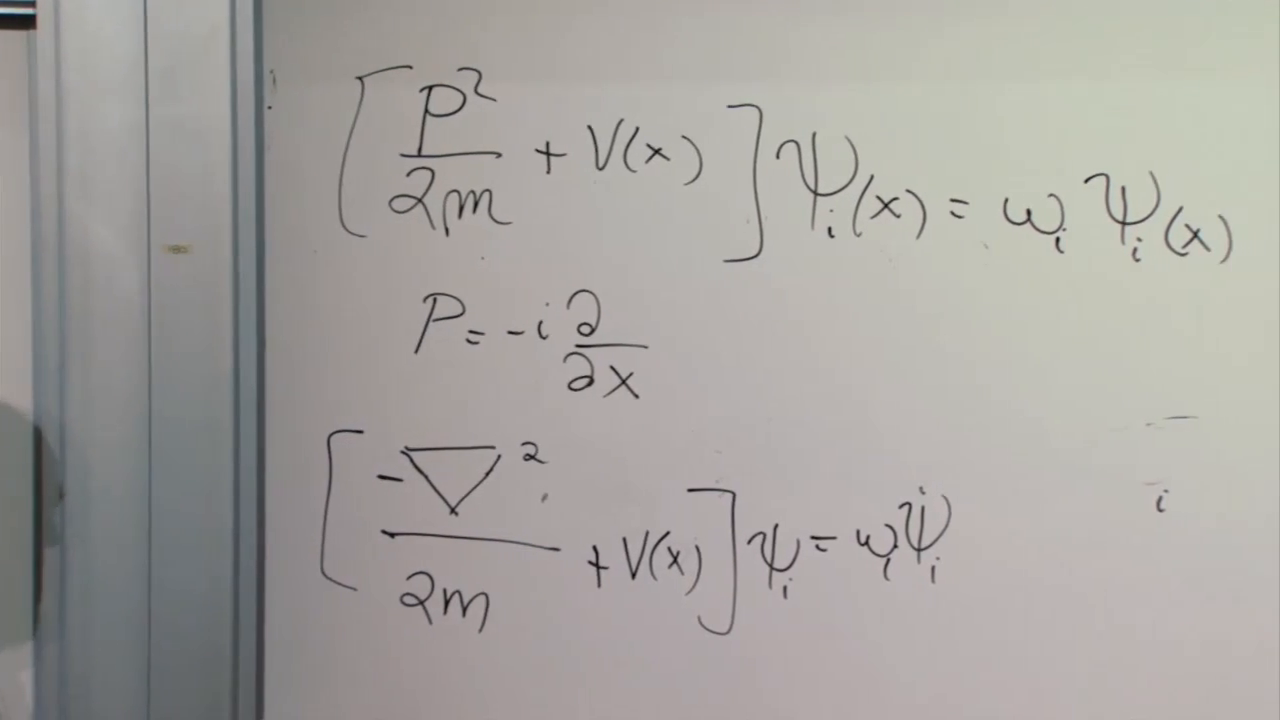
\includegraphics[width=0.94\linewidth]{lecture_07_frame_02.png}
\caption{黑板上從 \(p^2/(2m)+V(x)\) 推到單粒子薛丁格本徵值方程微分形式的過程。式~\eqref{eq:l07-schrodinger-eigenvalue}是整理後的重構版本。}
\lectureframe{00:54:10}
\end{figure}

對任意歸一化的單粒子波函數，熟知的能量期望值為
\begin{equation}
\langle h\rangle_\psi
=\int dx\,\psi^*(x)h\psi(x).
\label{eq:l07-one-particle-energy-expectation}
\end{equation}
多粒子公式可以從這個形式得到提示：把小寫的波函數換成算符值場。這還不是證明，而是我們接下來要檢驗的猜想：
\begin{equation}
H=\int dx\,\Psi^\dagger(x)h\Psi(x).
\label{eq:l07-field-hamiltonian}
\end{equation}

\section{先寫出答案，再加以證明}

將式~\eqref{eq:l07-field-expansion}代入所提出的哈密頓量：
\begin{align}
\int dx\,\Psi^\dagger h\Psi
&=\int dx
\left(\sum_i a_i^\dagger\psi_i^*(x)\right)
h\left(\sum_j a_j\psi_j(x)\right) \\
&=\sum_{i,j}a_i^\dagger a_j
\int dx\,\psi_i^*(x)h\psi_j(x).
\label{eq:l07-h-expanded}
\end{align}
微分算符 \(h\) 作用於依賴 \(x\) 的波函數 \(\psi_j(x)\)，而不是作用於模式算符 \(a_j\)。根據薛丁格方程，
\begin{equation}
h\psi_j(x)=\omega_j\psi_j(x).
\end{equation}
因此，
\begin{align}
\int dx\,\Psi^\dagger h\Psi
&=\sum_{i,j}a_i^\dagger a_j\omega_j
\int dx\,\psi_i^*(x)\psi_j(x) \\
&=\sum_{i,j}a_i^\dagger a_j\omega_j\delta_{ij} \\
&=\sum_j\omega_j a_j^\dagger a_j.
\label{eq:l07-h-proof}
\end{align}
這正是式~\eqref{eq:l07-mode-hamiltonian}。局部場的表示式與所有粒子能量的總和，是同一個算符。

\begin{figure}[htbp]
\centering
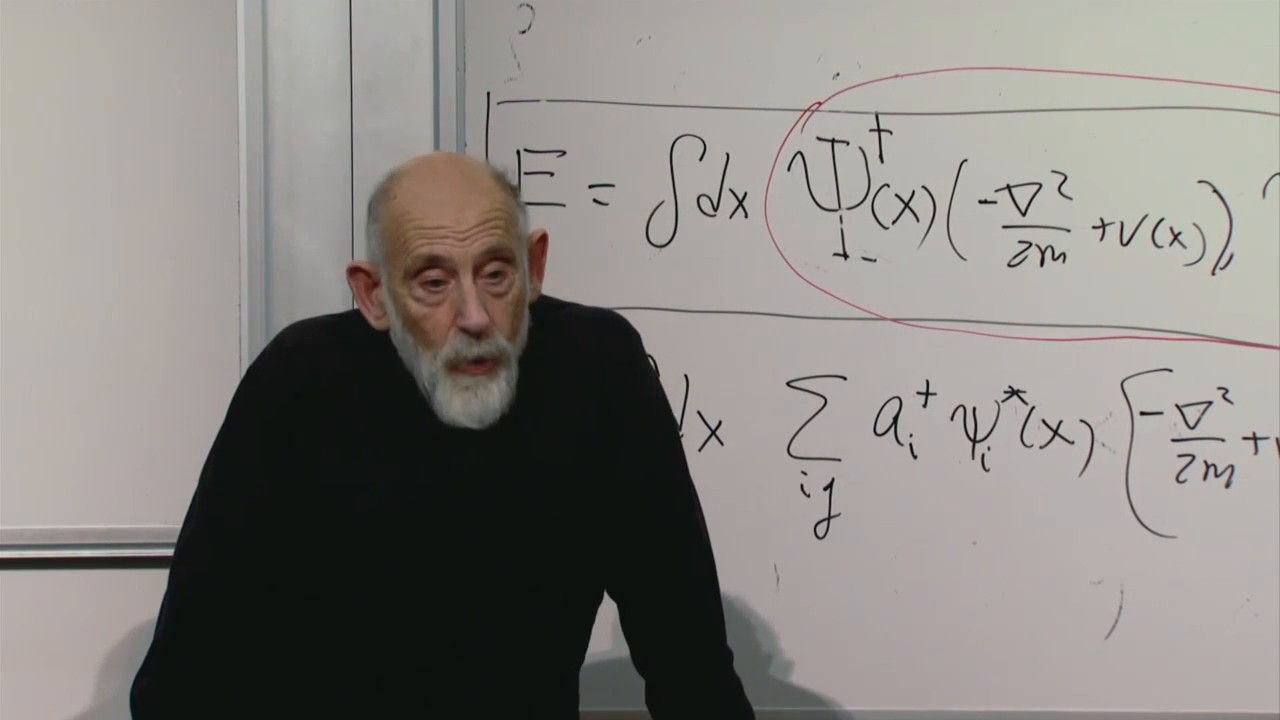
\includegraphics[width=0.94\linewidth]{lecture_07_frame_03.png}
\caption{黑板上著重標示的場哈密頓量，下方則開始以模式展開式進行證明。保留課堂畫面作為佐證；式~\eqref{eq:l07-field-hamiltonian}--\eqref{eq:l07-h-proof}補上完整的推導。}
\lectureframe{01:05:34}
\end{figure}

這段推導中，沒有把任何產生算符移過湮滅算符。\(a_i^\dagger a_j\) 的順序從頭到尾都保持不變。只有 \(c\) 數波函數及其本徵值可以任意移動。

\section{為什麼稱它為場}

為什麼稱 \(\Psi(x)\) 為場？因為它是在空間每一點定義的算符值量，而由它構成的厄米組合或雙線性算符則是局部可觀測量。密度 \(n(x)\) 與下文的局部能量表示式就是兩個例子。「場」這個詞背後沒有其他隱藏的數學判準。

這個場不是電磁場，而是描述提供單粒子模式與哈密頓量 \(p^2/(2m)+V\) 的非相對論性粒子種類，例如緩慢運動的原子、中子、質子或電子。這些粒子是各自對應場的量子；就結構而言，這與光子是電磁場的量子相同。

\begin{classroomqa}
\lecturetimestamp{01:02:45}
\audiencequestion{從多粒子系統推到上述公式時，場是在哪一步引入的？}
\lecturerresponse{場是在式~\eqref{eq:l07-field-expansion}引入的：\(\Psi(x)\)在每個空間位置都是一個算符。後續推導顯示，它的局部乘積可以測量粒子密度與能量密度。具有空間依賴性且包含算符，正是我們正在建構的場結構。}
\end{classroomqa}

\section{局部能量密度}

式~\eqref{eq:l07-field-hamiltonian}將總能量寫成空間積分：
\begin{equation}
\begin{aligned}
H&=\int dx\,\mathcal H(x),\\
\mathcal H(x)
&=-\frac{1}{2m}\Psi^\dagger(x)\nabla^2\Psi(x)\\
&\quad+V(x)\Psi^\dagger(x)\Psi(x).
\end{aligned}
\label{eq:l07-hamiltonian-density}
\end{equation}
被積項是這個哈密頓量自然的一種局部能量密度，但局部形式並不唯一。例如，分部積分可以把動能項改寫為
\begin{equation}
\mathcal H_{\rm kin}(x)
=\frac{1}{2m}\nabla\Psi^\dagger(x)\mathbin{\cdot}\nabla\Psi(x)
\label{eq:l07-kinetic-density}
\end{equation}
兩者只差一個邊界項。在通常的邊界條件下，這兩種表示式給出相同的總哈密頓量。這就是課堂上提到的那點不唯一性。

\begin{classroomqa}
\lecturetimestamp{01:05:57}
\audiencequestion{能量密度一定要在全空間積分嗎？}
\lecturerresponse{在全空間積分會得到總能量；在較小區域積分，則得到歸屬於該區域的能量。這仍受局部密度選取方式不唯一的影響，只要對全空間積分後得到相同的哈密頓量即可。}
\end{classroomqa}

\begin{classroomqa}
\lecturetimestamp{01:06:25}
\audiencequestion{能量公式中的大寫 \(N_i\) 與小寫 \(n_i\) 有何不同？}
\lecturerresponse{\(N_i=a_i^\dagger a_i\)是算符。整數 \(n_i\) 則是它在佔據數態上的其中一個本徵值。算符作用於態；本徵值則是普通數值。}
\end{classroomqa}

\begin{classroomqa}
\lecturetimestamp{01:06:46}
\audiencequestion{能否用狄拉克符號把場哈密頓量本身寫成左矢或右矢？}
\lecturerresponse{不能。左矢與右矢表示態向量及其對偶；場與哈密頓量則是作用於這些態的算符。像 \(\langle\Phi|H|\Phi\rangle\) 這樣的期望值同時涉及兩類對象，不應將兩者混為一談。}
\end{classroomqa}

\section{重現單粒子理論，並邁向經典場}

擴大的形式架構包含了普通的單粒子量子力學。將福克空間限制在滿足下式的態：
\begin{equation}
N|\Phi\rangle=|\Phi\rangle.
\end{equation}
在這個扇區中，場的構造會重現所有單粒子態與單粒子預測。我們並未取代舊理論，而是把它嵌入一個也能描述零個、兩個或任意多個粒子的空間中。

在另一個極端，若某個模式中有大量玻色子，它就可能近似呈現經典波的行為。在適當的相干態或半經典態中，期望值
\begin{equation}
\Phi_{\rm cl}(x,t)=\langle\Psi(x,t)\rangle
\end{equation}
對自由非相對論性理論滿足下列看似經典的方程：
\begin{equation}
i\partial_t\Phi_{\rm cl}(x,t)
=\left(-\frac{\nabla^2}{2m}+V(x)\right)\Phi_{\rm cl}(x,t)
\label{eq:l07-classical-schrodinger}
\end{equation}
課堂上指出這項關聯，但沒有加以推導。這是量子粒子集合與波場之間的橋梁：大量佔據會抑制相對漲落，使適當的期望值呈現經典行為。

因此，這套形式架構既是記帳工具，也是物理描述。它整理了所有粒子數扇區，也刻畫干涉、糾纏，以及經典波如何從量子粒子中浮現。

\begin{classroomqa}
\lecturetimestamp{01:10:43}
\audiencequestion{為什麼在積分中操作產生與湮滅算符時，幾乎可以把它們當成普通數值？}
\lecturerresponse{它們彼此從未交換順序。普通模式函數與這些算符對易，而導數只作用於那些函數。若要把湮滅算符移過產生算符，就必須使用對易子，也可能因此多出一項；但證明中的任何一步都沒有進行這種操作。}
\end{classroomqa}

\section{狄拉克符號小插曲}

有些混淆源自歷史背景。單粒子波函數滿足波動方程，表面上看似經典場，同時卻又是機率振幅。早期量子理論必須先區分這兩種角色，再說明電磁學這類真正可測量的波場如何由量子構成。福克空間與算符值場化解了這個表面上的矛盾。

狄拉克符號能以極精簡的方式呈現這種區別。右矢屬於向量空間，左矢屬於其對偶空間，兩者並置便構成內積。有了完備關係
\begin{equation}
\sum_i|i\rangle\langle i|=\mathbf 1
\end{equation}
整個過程幾乎一目了然。課堂上用一則向數學家講授量子力學的軼事說明這一點：數學內容原本就熟悉，但符號讓常見運算變得如此清楚，整體結構看起來竟像是新發現。重點不是哪個學科缺少這個概念，而是恰當的符號能讓合法的運算不易混淆。

這個道理在此很重要。現在有幾種不同的算符：
\begin{itemize}
\item \(h\) 作為微分算符作用於單粒子波函數；
\item \(a_i\) 和 \(a_i^\dagger\) 作用於福克空間中的佔據數態；
\item \(\Psi(x)\)、\(\Psi^\dagger(x)\)、\(N\) 與 \(H\) 也作用於福克空間。
\end{itemize}
式~\eqref{eq:l07-field-expansion}中的展開式連結了前兩種情境，但沒有把它們混為一談。

\begin{classroomqa}
\lecturetimestamp{01:18:16}
\audiencequestion{場只是描述粒子集合的一套形式架構嗎？}
\lecturerresponse{場論確實是一套形式架構，但並非空洞的形式。場的局部可觀測量可以測量；粒子則是具有干涉與糾纏的量子粒子，而非經典小球。場算符恰好編碼了這些可測量的集體性質。}
\end{classroomqa}

\section{相對論的提醒與電磁學旁論}

目前的構造是非相對論性的。在相對論物理中，動量仍是良好的粒子標記，但要嚴格局域化粒子位置則複雜得多。因此，局部光子數密度通常不像非相對論性的 \(n(x)\) 那樣明確。能量密度仍有良好定義，是較可靠的局部可觀測量。

課堂上提出一個有用、但明確僅供啟發的電磁類比。將電場與磁場組合成複向量：
\begin{equation}
\mathbf F=\mathbf E+i\mathbf B,
\qquad
\mathbf F^*=\mathbf E-i\mathbf B.
\label{eq:l07-riemann-silberstein}
\end{equation}
於是
\begin{equation}
\mathbf F^*\mathbin{\cdot}\mathbf F
=\mathbf E^2+\mathbf B^2,
\label{eq:l07-em-density}
\end{equation}
在慣用單位制下，它與電磁能量密度成正比。這並不是真正的光子機率密度。較恰當的看法是：它是能以模平方表示能量密度的精簡場變數；非正式地說，也可把它理解為以光子能量加權的光子密度。

\begin{classroomqa}
\lecturetimestamp{01:19:10}
\audiencequestion{光子密度能否等同於電場強度？}
\lecturerresponse{只能在定性層次上謹慎地這麼說。對相對論性光子而言，局部粒子數不是首選概念。可靠的說法是，\(E^2+B^2\) 與能量密度成正比，而複數組合 \(\mathbf E+i\mathbf B\) 則將馬克士威方程組寫成類似薛丁格方程的形式。}
\end{classroomqa}

\begin{classroomqa}
\lecturetimestamp{01:20:09}
\audiencequestion{為什麼相對論性粒子可以有確定動量，位置卻成問題？}
\lecturerresponse{動量能清楚標記相對論性單粒子表示；嚴格局域化則與粒子產生及相對論性場描述相牴觸。本講不會進一步發展這套理論；此處的提醒是要指出，目前非相對論性密度詮釋的適用界限。}
\end{classroomqa}

\section{算符排序與基態常數}

不能任意改變算符的順序。對玻色模式而言，
\begin{equation}
a_i a_i^\dagger=a_i^\dagger a_i+1.
\end{equation}
因此，將正規排序的 \(\Psi^\dagger h\Psi\) 改成反向排序的 \((h\Psi)\Psi^\dagger\)，或改成適當積分後的對應形式，都會多出對易子項。在模式基底中，這是一個對每個模式各加上一個能量量子的總和。這就是基態常數，也稱零點能常數；在連續情況下，還需要對它進行調節。本講不會進一步探討這個問題，只提醒兩種排序並不相等。

\begin{classroomqa}
\lecturetimestamp{01:22:04}
\audiencequestion{如果在哈密頓量中交換 \(\Psi\) 與 \(\Psi^\dagger\) 的順序，會發生什麼事？}
\lecturerresponse{必須計入它們的對易子。因此，顛倒順序會多出一項與態無關的基態貢獻，而不會得到相同的表示式。展示的哈密頓量採用正規序，\(\Psi^\dagger h\Psi\)。}
\end{classroomqa}

\section{動量作為最後的檢驗}

最後幾分鐘再次進行相同的提升。對單一粒子而言，
\begin{equation}
\langle p\rangle_\psi
=\int dx\,\psi^*(x)\left(-i\partial_x\right)\psi(x).
\label{eq:l07-one-particle-momentum}
\end{equation}
將波函數換成場，即得到總動量算符
\begin{equation}
P=\int dx\,\Psi^\dagger(x)\left(-i\partial_x\right)\Psi(x),
\label{eq:l07-field-momentum}
\end{equation}
在三維中則為
\begin{equation}
\mathbf P=\int d^3x\,\Psi^\dagger(\mathbf x)
\left(-i\boldsymbol\nabla\right)\Psi(\mathbf x).
\end{equation}
場會攜帶動量。足夠強的雷射會將動量傳遞給牆壁，並對牆壁施力；在量子描述中，場的動量就是所有光子動量的總和。

式~\eqref{eq:l07-field-momentum}是算符，不是期望值。給定一個 Fock 空間中的態 \(|\Phi\rangle\)，便可以計算
\begin{equation}
\langle P\rangle_\Phi=\langle\Phi|P|\Phi\rangle.
\end{equation}
要形成期望值，算符和態缺一不可。若把可觀測量與其平均值混為一談，就會抹去本講一直努力建立的區分。

\begin{classroomqa}
\lecturetimestamp{01:26:02}
\audiencequestion{展示的場動量已經是平均動量了嗎？}
\lecturerresponse{不是。它是代表該可觀測量的厄米算符。給定一個態，將算符夾在該態的左矢與右矢之間，才能得到期望值；測量結果仍可能在平均值附近有所漲落。}
\end{classroomqa}

這裡是自然的收尾。從粒子出發，我們構造了局域的產生場與湮滅場，用它們計數粒子，並將單粒子能量與動量的總和改寫為場算符。下一步不再只是改變記號，而是讓場算符描述物理過程：粒子衰變、粒子散射，以及不同種類的粒子彼此轉化。

\chapter{混合、振盪、電偶極矩與場算符}

我們先從一個稍微偏離本章主題的問題談起：中微子。有證據顯示中微子具有質量，而且不同種類的中微子會發生混合。如果它們的質量並不全都相同，為什麼一種中微子可以轉變成另一種，卻不違反能量守恆？

這個問題帶出量子力學中反覆出現的一種結構：製備或測量系統時所對應的態，不一定是讓哈密頓量對角化的態。確定能量的態只會獲得相位；若製備的態是數個能量本徵態的疊加，各分量因獲得不同相位，整個態便會改變。這個區別將帶我們從雙勢阱談到中微子振盪與自旋進動。接著我們會插談電子電偶極矩，再回到二次量子化，看看同樣的位置--動量傅立葉結構如何出現在算符層次。

\section{問題的核心是混合}

中微子的質量不必全都相同。能量本徵態彼此不會混合；每個本徵態都獨立演化。我們所說的中微子\emph{種類}，也就是味，與中微子的產生和測量方式有關；味態則可以是質量能量本徵態的線性組合。概略地說，
\begin{equation}
|\text{type}\rangle = \sum_n c_n |E_n\rangle .
\end{equation}
因此，正確的說法不是能量本徵態彼此轉變，而是稱為``電子中微子''或``{\proseunicodefont μ}子中微子''的態，本身不一定是能量本徵態。

\begin{classroomqa}
\lecturetimestamp{00:00:09}
\audiencequestion{如果中微子具有不同質量，它們如何能在能量守恆的情況下混合？}
\lecturerresponse{質量能量本徵態不會彼此轉變。電子味、{\proseunicodefont μ}子味和{\proseunicodefont τ}味態，是這些本徵態的不同線性組合。各質量分量分別依自己的相位演化；分量間的干涉會改變各味的機率，但不違反能量守恆。}
\end{classroomqa}

這種結構有許多例子。最直觀的一個例子，是粒子處於對稱雙勢阱中。

\section{對稱雙勢阱與近似定域態}

考慮一個粒子在對稱雙勢阱中運動，兩個勢阱最低點之間隔著一道高勢壘。若勢壘無限高，左右兩個勢阱便會完全解耦。我們可以把右側視為不存在，只求解左側勢阱；右側也可以同樣處理。近似的基態波函數便是左側定域態\(\psi_L\)與右側定域態\(\psi_R\)，兩者的能量相同\(E\)。

在每個孤立的勢阱中，基態都有熟悉的定性特徵：波函數平滑、沒有節點，並且處於符合束縛條件的最低能量。可以把中央的高勢壘想成一道磚牆。把它視為無限高只是近似，但能讓我們先從一對有用的定域態開始。

\begin{figure}
\centering
\begin{adjustbox}{max width=\linewidth}
\begin{tikzpicture}[x=0.8cm,y=0.8cm]
\begin{scope}[shift={(-5.8,0)}]
\draw (-4,2.7) .. controls (-3.35,1.2) and (-2.55,-0.45) .. (-2.0,-0.72)
      .. controls (-1.35,-0.95) and (-0.7,0.65) .. (0,2.05)
      .. controls (0.7,0.65) and (1.35,-0.95) .. (2.0,-0.72)
      .. controls (2.55,-0.45) and (3.35,1.2) .. (4,2.7);
\draw[dashed] (-4,-0.10) -- (4,-0.10);
\node at (-3.55,-0.48) {$E$};
\draw[line width=0.9pt] (-4,-0.02) .. controls (-3.2,-0.02) and (-2.7,0.30) .. (-2.15,0.95)
      .. controls (-1.55,1.30) and (-1.15,0.35) .. (-0.55,-0.06)
      .. controls (0.15,-0.14) and (0.9,-0.15) .. (4,-0.15);
\node at (-2.15,1.35) {$\psi_L$};
\end{scope}
\begin{scope}[shift={(5.8,0)}]
\draw (-4,2.7) .. controls (-3.35,1.2) and (-2.55,-0.45) .. (-2.0,-0.72)
      .. controls (-1.35,-0.95) and (-0.7,0.65) .. (0,2.05)
      .. controls (0.7,0.65) and (1.35,-0.95) .. (2.0,-0.72)
      .. controls (2.55,-0.45) and (3.35,1.2) .. (4,2.7);
\draw[dashed] (-4,-0.10) -- (4,-0.10);
\node at (-3.55,-0.48) {$E$};
\draw[line width=0.9pt] (-4,-0.02) .. controls (-3.2,-0.01) and (-2.7,0.30) .. (-2.15,0.95)
      .. controls (-1.6,1.28) and (-1.1,0.25) .. (-0.30,-0.08)
      .. controls (0.35,-0.12) and (0.85,-0.12) .. (1.35,0.35)
      .. controls (1.9,0.88) and (2.35,1.15) .. (2.85,0.55)
      .. controls (3.2,0.05) and (3.55,-0.12) .. (4,-0.15);
\end{scope}
\end{tikzpicture}
\end{adjustbox}
\caption{開場板書草圖的清晰重繪。左圖是單側試探態\(\psi_L\)，是把勢壘視為實際上無限高時得到的結果。右圖則將同一波函數對稱地延伸至勢壘另一側，顯示波函數有少量但非零的穿透，最終形成真正的偶宇稱基態。}
\end{figure}

然而，在量子力學中，勢壘並非真正無限高。勢壘區域中的波函數不會恰好等於零，只是非常小。這一點微弱的穿透正是關鍵所在；它使左右兩側的近似描述成為真正的混合問題。

\section{宇稱本徵態與指數級能階分裂}

現在，定域態的圖像要讓位給一個定理：若位勢具有對稱性，精確的能量本徵函數就可以選成在反射下為對稱態或反對稱態。

\begin{theorem}
若一維位勢滿足\(V(x)=V(-x)\)，則哈密頓量的本徵函數可以選成滿足以下其中一種關係：
\[
\psi(x)=\psi(-x)
\qquad \text{or} \qquad
\psi(x)=-\psi(-x).
\]
\end{theorem}

接著要修正先前的近似。單側態\(\psi_L\)與\(\psi_R\)既不對稱，也不反對稱，因此不可能是完整哈密頓量的精確本徵態。只有在勢壘很高時，它們才是良好的近似態。真正的本徵態是對稱與反對稱的線性組合：
\begin{align}
\psi_+ &= \frac{\psi_L+\psi_R}{\sqrt{2}},\\
\psi_- &= \frac{\psi_L-\psi_R}{\sqrt{2}}.
\end{align}
沿用留在黑板上的記號，將它們的能量標為
\begin{align}
H\psi_+ &= (E_1-\epsilon)\psi_+,\\
H\psi_- &= (E_1+\epsilon)\psi_-.
\end{align}
因此，兩能階的總分裂為
\begin{equation}
\Delta E = (E_1+\epsilon)-(E_1-\epsilon)=2\epsilon .
\end{equation}

\begin{figure}[htbp]
\centering
\includegraphics[width=0.92\linewidth]{lecture_08_frame_02.png}
\caption{雙勢阱中的對稱延伸波函數。波函數在勢壘下方的振幅雖小但不為零，能階分裂正是由此而來。}
\lectureframe{00:06:19}
\end{figure}

\begin{figure}
\centering
\begin{tikzpicture}[x=1cm,y=1cm]
\draw[->] (0,0) -- (0,3);
\node[left] at (0,2.8) {energy};
\draw (-0.35,1.60) -- (0.35,1.60);
\node[left] at (-0.45,1.60) {$\psi_L,\psi_R$};
\node at (1.7,1.60) {$\Longrightarrow$};
\draw (3.0,1.32) -- (3.75,1.32);
\draw (3.0,1.88) -- (3.75,1.88);
\draw[dashed] (2.8,1.60) -- (3.95,1.60);
\node[right] at (3.9,1.32) {$\psi_+,\ E_1-\epsilon$};
\node[right] at (3.9,1.88) {$\psi_-,\ E_1+\epsilon$};
\node[below] at (3.37,1.60) {$E_1$};
\end{tikzpicture}
\caption{隧穿分裂的板書推導。近似的左側態與右側態幾乎簡併，但精確的對稱與反對稱本徵態之間仍有微小能量差\(2\epsilon\)。}
\end{figure}

能階的高低順序反映了其中的物理。對稱態的能量稍低，因為它在勢壘區域較平滑；波函數得以穿透勢壘並對稱延伸，會使能量降低一點點。反對稱態的能量稍高，因為一維系統的第一激發態有一個節點，而在這個對稱問題中，節點位於中點。額外的曲率會增加動能。

這個效應非常小，而且隨勢壘的寬度與高度呈指數級變小。這裡不需要寫出明確的 WKB 公式；重要的是，能階分裂確實存在，只是非常微小。另外要記得，波函數的整體正負號不具物理意義。將\(\psi_-\)換成\(-\psi_-\)，不會改變這個態。

\section{時間演化與左右振盪}

現在來問動力學問題：若一開始把粒子置於左側勢阱，會發生什麼事？這是關鍵的一步，因為振盪正是同一混合現象在時間演化中的呈現。

反向關係為
\begin{align}
\psi_L &= \frac{\psi_+ + \psi_-}{\sqrt{2}},\\
\psi_R &= \frac{\psi_+ - \psi_-}{\sqrt{2}}.
\end{align}
因此，初始時局域在左側的態是
\begin{equation}
\psi(0)=\psi_L=\frac{\psi_+ + \psi_-}{\sqrt{2}}.
\end{equation}
它不是能量本徵態，所以必然會發生非平凡的時間演化。

我們採用標準的Schr\"odinger約定\(e^{-iEt}\)。共同相位不會造成可觀測效應；只有兩個能量分量之間的相對相位，才能使機率從一個勢阱轉移到另一個勢阱。

依照這個約定，
\begin{equation}
\psi(t)=\frac{1}{\sqrt{2}}\left(e^{-i(E_1-\epsilon)t}\psi_+ + e^{-i(E_1+\epsilon)t}\psi_-\right).
\end{equation}
這是整理後的板書公式。現在提出共同相位：
\begin{equation}
\psi(t)=\frac{e^{-iE_1 t}}{\sqrt{2}}\left(e^{i\epsilon t}\psi_+ + e^{-i\epsilon t}\psi_-\right).
\end{equation}
此時，一個相位沿單位圓朝一個方向變化，另一個則朝相反方向變化。態之所以改變，只是因為兩個相位逐漸不同步。

將\(\psi_\pm\)的定義代入，就能明確看出左右振盪：
\begin{align}
\psi(t)
&= \frac{e^{-iE_1 t}}{2}
\left[e^{i\epsilon t}(\psi_L+\psi_R)+e^{-i\epsilon t}(\psi_L-\psi_R)\right] \\
&= \frac{e^{-iE_1 t}}{2}
\left[(e^{i\epsilon t}+e^{-i\epsilon t})\psi_L+(e^{i\epsilon t}-e^{-i\epsilon t})\psi_R\right] \\
&= e^{-iE_1 t}\left[\psi_L\cos(\epsilon t)+i\,\psi_R\sin(\epsilon t)\right].
\end{align}
這是本章的關鍵推導。在雙態近似下，若\(\psi_L\)與\(\psi_R\)正交歸一，兩側的機率為
\begin{equation}
P_L(t)=\cos^2(\epsilon t),
\qquad
P_R(t)=\sin^2(\epsilon t).
\end{equation}
因此，系統會振盪。在兩端之間的時刻，系統確實處於疊加態；例如，當\(\epsilon t=\pi/4\)時，粒子在兩側的機率相等。相位連續演化，定域程度也隨之連續改變。

黑板上的推導找出相對符號第一次反轉的時刻，也就是滿足下式的時刻：
\begin{equation}
e^{-i\epsilon t}=-\,e^{i\epsilon t},
\end{equation}
這是板書中清楚標出的關鍵條件。兩邊同乘後得到
\begin{equation}
e^{2i\epsilon t}=-1.
\end{equation}
第一次出現這種情況時，
\begin{equation}
2\epsilon t=\pi,
\qquad\text{so}\qquad
t_{L\to R}=\frac{\pi}{2\epsilon}.
\end{equation}

\begin{figure}[htbp]
\centering
\includegraphics[width=0.94\linewidth]{lecture_08_frame_05.png}
\caption{黑板上的相對相位計算。當\(e^{2i\epsilon t}=-1\)時，兩個能量分量的相位相差{\proseunicodefont π}，得到第一次轉移所需時間\(2\epsilon t=\pi\)。排版後的推導一致採用Schr\"odinger相位約定。}
\lectureframe{00:17:52}
\end{figure}
在這個時刻，
\begin{equation}
\psi(t_{L\to R}) \propto \frac{\psi_+-\psi_-}{\sqrt{2}}=\psi_R.
\end{equation}
整體相位無關緊要。重要的是，起初置於左側的粒子已演化成右側定域態。再經過同樣長的時間，它便會擺回左側。混合與振盪相伴而生。

方程所表示的結果很明確：\(\epsilon\)越小，振盪越慢，轉移所需時間越長。兩個定域態都沒有確定的能量；但兩個精確的能量分量各自守恆能量，並依照應有的方式演化。

\section{中微子、氨分子與自旋的類比}

雙勢阱提供了一個理解中微子問題的範例。與電子一同產生的中微子稱為電子中微子；與{\proseunicodefont μ}子一同產生的則稱為{\proseunicodefont μ}子中微子。這些味標籤描述產生與測量的通道。具有確定質量的態構成另一組基底；在動量固定時，它們也具有確定的自由粒子能量。

在最簡單的雙態最大混合示意模型中，
\begin{equation}
|\nu_e\rangle \sim \frac{|m_1\rangle+|m_2\rangle}{\sqrt{2}},
\qquad
|\nu_\mu\rangle \sim \frac{|m_1\rangle-|m_2\rangle}{\sqrt{2}},
\end{equation}
其中，質量本徵態對應\(\psi_+\)與\(\psi_-\)，味態則對應\(\psi_L\)與\(\psi_R\)。真實的中微子混合由非平凡的混合矩陣描述，係數並不相等；不過，這裡已能看出其作用機制。

電子中微子是在涉及電子的過程中產生的，就像粒子一開始被置於左側勢阱。在短距離傳播後，它的兩個質量分量所累積的相位幾乎相同，因此仍會在交互作用中被辨識為電子味。經過長距離傳播後，兩個相位便會分開。之後的帶電流交互作用可能產生{\proseunicodefont μ}子而非電子，表示該態已含有{\proseunicodefont μ}子味分量。在不同距離或能量下重複實驗，就能觀察到振盪。

這並不違反能量守恆。質量能量本徵態完全依照本徵態應有的方式演化；隨時間改變的是味疊加態。在相對論極限下，可觀測的相對相位取決於質量平方差，概略地說：
\begin{equation}
\Delta\phi_{ij}\simeq \frac{\Delta m_{ij}^{,2}L}{2E}.
\end{equation}
因此，觀察到振盪表示中微子的質量不可能全都相同；至少有兩個質量本徵態的質量不同。

\begin{classroomqa}
\lecturetimestamp{00:24:06}
\audiencequestion{雙勢阱例子中的微小能階分裂\(\epsilon\)由什麼決定？}
\lecturerresponse{它取決於粒子質量，以及勢壘的高度與寬度。隧穿對這些細節呈指數敏感，因此勢壘稍有變化，就可能使\(\epsilon\)的相對大小大幅改變。}
\end{classroomqa}

\begin{classroomqa}
\lecturetimestamp{00:24:26}
\audiencequestion{這種振盪現象真的觀測到了嗎？}
\lecturerresponse{是的。一般量子系統中觀測得到隧穿造成的能階分裂，中微子則有味振盪。兩者的微觀機制不同，但都呈現相同的雙態相位演化。}
\end{classroomqa}

\begin{classroomqa}
\lecturetimestamp{00:24:34}
\audiencequestion{中微子振盪與中微子質量有什麼關聯？}
\lecturerresponse{傳播中的本徵態具有不同質量，因此累積的相位也不同。這些分量彼此干涉，改變了味的組成。在符合實際情況的相對論描述中，控制振盪的是質量平方差，而不是單一粒子的質量真的隨時間變化。}
\end{classroomqa}

\begin{classroomqa}
\lecturetimestamp{00:25:02}
\audiencequestion{中微子質量只是主流理論的說法，還是實驗事實？}
\lecturerresponse{振盪是實驗事實，而且要求質量差不為零。絕對質量尺度是另一個更難測量的問題，但「所有中微子都沒有質量」這個最簡單的圖像已被實驗排除。}
\end{classroomqa}

\subsection{氨分子反轉：真實的勢壘}

氨分子\(\mathrm{NH}_3\)呈三角錐形：三個氫原子位於同一平面，氮原子則位於平面一側。氮原子位於另一側時，也有一個等價構型。這兩個定域構型都不是精確的定態。氮原子可以隧穿穿過氫原子所在的平面，形成對稱與反對稱的能量本徵態，並造成微小的反轉能階分裂。氨微波激射器中的相關數學結構，物理上正是源自這個效應。

\begin{classroomqa}
\lecturetimestamp{00:25:11}
\audiencequestion{在氨分子中，勢壘是否就是氮原子穿過氫原子所在平面時的構型？}
\lecturerresponse{是。分子在兩種三角錐構型下的能量都最低，平面構型的能量則較高。氮原子隧穿經過這個構型，便會耦合兩側。}
\end{classroomqa}

\begin{classroomqa}
\lecturetimestamp{00:27:10}
\audiencequestion{電子中微子與{\proseunicodefont μ}子中微子之間，對應的實際勢壘是什麼？}
\lecturerresponse{這裡沒有字面上的空間勢壘。這個類比只在代數結構上成立：中微子哈密頓量中的非對角耦合會使味基底發生混合。在氨分子中，這種耦合來自隧穿；對中微子而言，它是質量與混合結構的一部分。}
\end{classroomqa}

\subsection{自旋進動：不經由隧穿的混合}

我們已在自旋問題中見過相同的代數結構。考慮兩個態\(|\uparrow_z\rangle\)與\(|\downarrow_z\rangle\)。沒有磁場時，兩者能量簡併。現在施加沿\(x\)方向的磁場。能量本徵態不再是\(z\)本徵態，而是沿\(x\)方向偏極的態。沿用黑板上暫時採用的左--右標記，
\begin{align}
|L_x\rangle &= \frac{|\uparrow_z\rangle+|\downarrow_z\rangle}{\sqrt{2}},\\
|R_x\rangle &= \frac{|\uparrow_z\rangle-|\downarrow_z\rangle}{\sqrt{2}}.
\end{align}
這兩個態分別直接類比於\(\psi_+\)與\(\psi_-\)。磁矩沿磁場方向與反磁場方向排列時，能量略有差異。若能量為\(E\mp\epsilon\)，則初始朝上的自旋會演化為
\begin{equation}
|\uparrow_z,t\rangle
= e^{-iEt}\left[\cos(\epsilon t)\,|\uparrow_z\rangle
+ i\sin(\epsilon t)\,|\downarrow_z\rangle\right].
\end{equation}
這與雙勢阱的公式相同，只是此處的連續演化是自旋繞\(x\)軸進動。從\(+z\)出發，自旋會經過橫向取向，在半個進動週期後到達\(-z\)，再經過半個週期回到原處。測量\(S_z\)仍只會得到向上或向下；自旋態連續的變化決定了各結果的機率。這種機制不需要隧穿，只需要哈密頓量在不同於製備基底的另一組基底中為對角形式。

\begin{classroomqa}
\lecturetimestamp{00:32:25}
\audiencequestion{在這個圖像中，{\proseunicodefont τ}中微子會如何？}
\lecturerresponse{它也會發生混合。真實情況中有三種味態與三種質量態，因此要以三乘三混合矩陣取代雙態旋轉；相位干涉原理則維持不變。}
\end{classroomqa}

\begin{classroomqa}
\lecturetimestamp{00:32:57}
\audiencequestion{施加橫向磁場後，自旋會立刻仍朝上嗎？它能指向我們或背向我們嗎？}
\lecturerresponse{在極短時間內，自旋仍幾乎確定朝上，只有很小的機率朝下。此態會繞磁場軸連續進動，並經過橫向的\(\pm y\)方向；若它起初垂直於沿\(x\)方向的磁場，進動過程中仍會保持垂直。沿任何選定軸測量，結果仍是該軸的一個離散本徵值。}
\end{classroomqa}

\begin{classroomqa}
\lecturetimestamp{00:34:30}
\audiencequestion{選用弱磁場，是為了避免自旋指向磁場方向嗎？}
\lecturerresponse{不是。自旋的幾何變化源自繞磁場軸進動，與磁場強弱無關。弱磁場只會使能階分裂和進動頻率變小，因此振盪較慢，類似中微子的例子。}
\end{classroomqa}

中微子混合的強度與微小的中微子質量，其更深層的起源並未由最初形式的最小標準模型解釋。因此，中微子質量指向最小標準模型以外的物理。雖然觀測到的質量尺度非常小，仍可能反映了遙遠能量尺度上的物理。

\begin{classroomqa}
\lecturetimestamp{00:36:27}
\audiencequestion{我們是因為觀察到振盪，才知道中微子有質量嗎？}
\lecturerresponse{這是傳播分量具有不同質量的關鍵直接證據。若所有相關分量都嚴格無質量且彼此簡併，它們就不會累積依賴質量的相對相位，也不會出現這種真空味振盪。}
\end{classroomqa}

\begin{classroomqa}
\lecturetimestamp{00:37:57}
\audiencequestion{經過半個週期後，中微子是否應該一半是電子味、一半是{\proseunicodefont μ}子味？}
\lecturerresponse{在理想的對稱雙態模型中，兩種味的機率會在完整機率週期的四分之一處相等；完全轉換則發生在第一次機率極大值處。真實的三味振盪具有不相等的混合角、數種振盪頻率、自旋螺旋度限制與物質效應，因此一般不會出現完全對稱的轉換。}
\end{classroomqa}

\begin{classroomqa}
\lecturetimestamp{00:38:36}
\audiencequestion{若質量分量不同，太陽中微子的速度是否必須改變，才能守恆動量？}
\lecturerresponse{味態是由質量固定的分量構成的相干疊加；它的質量不是隨時間振盪的經典量。在常用的等動量描述中，各分量的能量與群速度略有不同；在等能量描述中，各分量的動量略有不同。只要處理方式一致，兩種描述都會得到相同的可觀測振盪相位。}
\end{classroomqa}

這種相位演化解釋了過去的太陽中微子缺失問題。早期探測器主要對電子中微子敏感，因此以電子味離開太陽的中微子，抵達時可能已部分轉為{\proseunicodefont μ}子味或{\proseunicodefont τ}味，因而不會被該通道偵測到。完整的太陽中微子計算包含三味混合與物質效應，但雙勢阱已呈現出核心概念：製備態與傳播所採用的基底不同。

\section{插曲：電偶極矩、對稱性與``「電子是球體」''的說法}

既然談到粒子唯象學，我們暫且放下形式數學，來看一個例子。一篇科普文章用「電子已被證明是球體」來描述一項新的電子電偶極矩上限。這種說法混淆了三個不同問題：電偶極矩測量的是什麼、旋轉對稱性對量子態有何意義，以及實驗實際限制了什麼。

\subsection{測量了什麼？}

實際測量的，或者更精確地說，實際設定上限的，是電子的電偶極矩。對於分離的電荷\(\pm q\)，偶極矩為
\begin{equation}
\mathbf d = q\,\boldsymbol{\ell},
\end{equation}
其中，\(\boldsymbol{\ell}\)是分離向量。電偶極矩不為零，表示電荷分布相對於某個中心有所偏移。

然而，對電子而言，關鍵不只是電荷是否沿某個任意方向偏離中心。電子具有自旋，因此有一個軸向；它也具有磁矩。真正有物理意義的問題，是電荷偏移是否與這個軸向相關：
\begin{equation}
\mathbf d_e \parallel \boldsymbol{\mu}_e
\qquad \text{or equivalently} \qquad
\mathbf d_e \parallel \mathbf S .
\end{equation}
這種相關性就是電子電偶極矩所指的物理量。概念上，我們要問的是：將自旋極化的電子置於電場中，兩種自旋取向是否會產生能量分裂？
\begin{equation}
H_{\mathrm{EDM}}=-\mathbf d_e\cdot \mathbf E,
\qquad
\mathbf d_e=d_e\frac{\mathbf S}{|\mathbf S|}.
\end{equation}
實際的桌上型實驗遠比把一顆裸電子放在電容器極板間來得精巧，但它運用的正是這種對稱性與能量位移的概念。

\subsection{沒有電偶極矩，為何不代表電子是球體}

第一個修正很簡單：物體即使沒有偶極矩，也不一定是球形。置中橢球兩側的電荷量相同，因此沒有偶極矩，但仍可能有四極矩。更複雜的電荷分布可能既沒有偶極矩，也沒有四極矩，卻仍具有更高階的多極矩。測量一個多極矩係數，無法確定整個形狀。

在量子力學中，``形狀''這個詞的意義更微妙。想像一個雙原子分子，像啞鈴一樣，鍵長近似固定。忽略徑向振動，只考慮轉動。它的轉動態以角動量標記。若分子是玻色子，最低轉動態的角動量為\(J=0\)。角動量是轉動的生成元，因此
\begin{equation}
\begin{gathered}
J=0 \quad\Longrightarrow\\
\text{rotationally invariant ground state.}
\end{gathered}
\end{equation}
即使每個確定取向的圖像都像啞鈴，這個量子態仍具有轉動不變性。也可以把它描述為所有取向的相干疊加。稱這個態為``球形''，對某些測量有用，對另一些測量則會造成誤解。

快速拍下一張快照。快照是對取向進行測量；足夠精確的取向測量會使系統處於角度局域的態。這種態不可能同時具有確定的角動量。這是位置--動量不確定性原理在轉動問題中的對應形式：角度局域必然帶來角動量分布的展寬，因此也會引入轉動激發。

對剛性轉子而言，
\begin{equation}
E_J=\frac{J(J+1)}{2I},
\end{equation}
因此，可分辨能量由轉動慣量\(I\)決定。體育館裡的啞鈴具有極大的\(I\)，轉動能階間距也極小；普通光線很容易擾動它，足以顯示其取向。分子的能階間距較大，緻密強子的能階間距則大得多。若探針能量不足以激發第一個可分辨的轉動結構，反覆測量看到的就只有經轉動平均後的基態。

介子可以粗略想成由夸克--反夸克組成的二體系統。其第一個軌道激發態所需能量至少達數億電子伏特，遠高於光學光子的能量。因此，低能探針無法拍下其內在取向的快照。``是否為球體''，部分取決於製備的是哪個態，部分取決於儀器的解析度。

電子讓這個問題更為明確。它是自旋為\(\tfrac12\)的粒子，不是轉動純量。自旋極化態具有一個軸向與磁矩。電荷繞該軸環流的熟悉圖像只是啟發性的示意---點狀狄拉克粒子並非字面上的微型旋轉球體---但這個圖像確實提醒我們，磁矩會隨自旋反向。電偶極矩所問的，是電荷偏移是否與同一軸向相關。測量結果為零，並不會使電子成為經典球體。

\begin{classroomqa}
\lecturetimestamp{00:57:30}
\audiencequestion{若電子的一部分電荷發生偏移，會違反電荷量子化嗎？}
\lecturerresponse{不會。電荷量子化限制的是總電荷。電偶極矩涉及電荷分布的一階空間矩；等價地說，它也可以描述點粒子與電場之間的一種允許耦合。這並不表示總電荷發生了分數變化。}
\end{classroomqa}

\begin{classroomqa}
\lecturetimestamp{00:58:00}
\audiencequestion{量子場論是否禁止電偶極矩？}
\lecturerresponse{量子場論本身並不禁止電偶極矩。若特定離散對稱性嚴格成立，電偶極矩才會受到禁止。對稱性一旦破壞，電偶極矩算符便是允許的，只是其係數可能極其微小。}
\end{classroomqa}

\subsection{宇稱與時間反演}

電偶極矩問題的核心在於對稱性。在宇稱變換下，電偶極矩的變換方式如同極向量，磁矩則如同軸向量：
\begin{align}
P:\qquad &\mathbf d_e \to -\mathbf d_e,
&\boldsymbol{\mu}_e \to \boldsymbol{\mu}_e .
\end{align}
在時間反演下，形成磁矩的環流會反向，靜態電荷位移則不變：
\begin{align}
T:\qquad &\mathbf d_e \to \mathbf d_e,
&\boldsymbol{\mu}_e \to -\boldsymbol{\mu}_e .
\end{align}
因此，若宇稱對稱性嚴格成立，平行於電子自旋軸的非零電偶極矩就會被禁止；時間反演對稱性嚴格成立時也同樣如此：
\begin{equation}
(P\ \text{exact}) \Rightarrow \mathbf d_e=0,
\qquad
(T\ \text{exact}) \Rightarrow \mathbf d_e=0.
\end{equation}

這個幾何關係值得仔細說明。磁矩由環狀電流產生。鏡射會反轉普通的極向量，卻不會改變該電流環路法向的軸向量。沿軸向的電荷位移則會反轉。因此，若電子的 \(\mathbf d_e\) 平行於 \(\boldsymbol\mu_e\)，鏡射後會得到一個磁取向相同、但電偶極矩與磁矩關係相反的電子。若宇稱是嚴格對稱性，且電子只有一種，那麼這兩種描述必須代表同一個粒子；只有 \(d_e=0\) 符合這個要求。

時間反演會以另一種方式得到相同結論。將影片倒轉播放會使電流反向，因此也使 \(\boldsymbol\mu_e\) 反向；但靜態電荷位移不會因此移動。磁矩平行的狀態會變成磁矩反平行的狀態。若時間反演是嚴格對稱性，同樣必須有 \(d_e=0\)。

\begin{figure}[htbp]
\centering
\begin{tikzpicture}[>=Stealth,scale=0.95]
  \node[font=\bfseries] at (1.0,2.25) {original};
  \draw[->,very thick,blue!70!black] (0.65,0) -- (0.65,1.65);
  \draw[->,very thick,red!75!black] (1.35,0) -- (1.35,1.65);
  \node[blue!70!black,below] at (0.65,0) {$\boldsymbol\mu$};
  \node[red!75!black,below] at (1.35,0) {$\mathbf d$};

  \node[font=\bfseries] at (4.5,2.25) {parity};
  \draw[->,very thick,blue!70!black] (4.15,0) -- (4.15,1.65);
  \draw[->,very thick,red!75!black] (4.85,1.65) -- (4.85,0);
  \node[blue!70!black,below] at (4.15,0) {$\boldsymbol\mu$};
  \node[red!75!black,below] at (4.85,0) {$-\mathbf d$};

  \node[font=\bfseries] at (8.0,2.25) {time reversal};
  \draw[->,very thick,blue!70!black] (7.65,1.65) -- (7.65,0);
  \draw[->,very thick,red!75!black] (8.35,0) -- (8.35,1.65);
  \node[blue!70!black,below] at (7.65,0) {$-\boldsymbol\mu$};
  \node[red!75!black,below] at (8.35,0) {$\mathbf d$};
\end{tikzpicture}
\caption{根據黑板上的論證重建的對稱性檢驗。宇稱會反轉電偶極矩，但不會反轉軸向量磁矩；時間反演會反轉磁矩，但不會反轉靜態電位移。任何一種嚴格對稱性都會禁止永久電偶極矩平行於自旋。}
\end{figure}

\begin{figure}[htbp]
\centering
\includegraphics[width=0.94\linewidth]{lecture_08_frame_06.png}
\caption{時間反演論證中，磁軸與電荷位移成對出現的草圖。上方簡潔的 TikZ 圖將變換的內容單獨呈現，方便與部分遭擦除的現場板書區分。}
\lectureframe{01:06:10}
\end{figure}

\begin{classroomqa}
\lecturetimestamp{01:06:38}
\audiencequestion{時間反演會使電流和電荷都反向嗎？}
\lecturerresponse{電流會反向，因為速度會反向；電荷本身不會反向。反轉電荷符號的是電荷共軛 \(C\)，而不是時間反演 \(T\)。}
\end{classroomqa}

\begin{classroomqa}
\lecturetimestamp{01:07:01}
\audiencequestion{時間反演具有反么正性，是否表示非相對論量子力學不具有時間反演不變性？}
\lecturerresponse{不是。反么正性正是量子力學中一致地表示時間反演的方式：它會對振幅取複共軛，並反轉動量和自旋。特定哈密頓量是否保持不變，是另一個問題。}
\end{classroomqa}

\begin{classroomqa}
\lecturetimestamp{01:07:19}
\audiencequestion{討論電偶極矩是否要求電子具有有限體積，而非為點粒子？}
\lecturerresponse{不需要。點粒子的有效哈密頓量可以包含 \(-d_e\,\widehat{\mathbf S}\!\cdot\!\mathbf E\)。實驗要測量的是相反自旋取向是否在電場中具有不同能量；不必實際解析延展的電荷雲。}
\end{classroomqa}

宇稱不是弱相互作用的對稱性；弱相互作用的手徵耦合會以最大程度違反宇稱。時間反演也不是嚴格對稱性，但標準模型中已知的時間反演破壞對電子電偶極矩的貢獻極其微小。雖然可以計算出非零的標準模型貢獻，但其數值遠低於此處討論的靈敏度。因此，零結果與標準模型相符，同時也對標準模型的延伸形成限制---例如超對稱以及其他可能產生更大時間反演破壞的新相互作用---。

基本的實驗構想很簡單。磁場會使不同自旋取向的能量分裂，藉此顯示磁偶極矩。電場則會造成額外的自旋相關能量位移，藉此顯示電偶極矩。實際的精密實驗會使用原子或分子、較長的相干進動時間、反轉外加場，並仔細控制系統誤差，而不是把孤立電子放進過度簡化的裝置中。

\begin{classroomqa}
\lecturetimestamp{01:11:02}
\audiencequestion{搜尋電偶極矩是高能碰撞實驗，還是使用物質樣品的實驗？}
\lecturerresponse{這是精密的桌上型物理實驗：電子束縛在受控的原子或分子環境中，並配合電場和磁場進行測量。實驗能量雖低，卻能藉由對微小對稱性破壞所造成位移的高度靈敏度，間接探測高能新物理。}
\end{classroomqa}

\begin{classroomqa}
\lecturetimestamp{01:12:21}
\audiencequestion{零結果是否會限制標準模型有哪些修改仍然可行？}
\lecturerresponse{原則上會：每個模型都會預測一個係數，因此對應到某個參數區域。要得出詳細的數值排除範圍，需要專門計算；但一般原理很明確---與標準模型在更高精度下相符，會縮小那些預測較大電偶極矩的替代模型可行的空間。}
\end{classroomqa}

\begin{classroomqa}
\lecturetimestamp{01:13:09}
\audiencequestion{量子資訊守恆是否需要時間反演對稱性？}
\lecturerresponse{不需要。即使哈密頓量不具有 \(T\) 對稱性，么正的時間演化仍會守恆資訊。固定磁場中的粒子就是熟悉的例子：在時間反演後的影片中，除非磁場也反轉，否則磁場會選定一個取向；然而量子演化依然是么正的。在局域且具洛倫茲不變性的量子場論之通常假設下，\(CPT\)聯合變換是一種對稱性，但么正性並不是由它來保證的。}
\end{classroomqa}

休息時間可以到此結束。零測量結果表示，在所述靈敏度範圍內，尚未探測到電子的電偶極矩。這不表示電子是球體，也不會推翻標準模型；它讓某些偏離標準模型的提案更難成立。

\section{回到二次量子化：傅立葉變換、動量模態與局域性}

我們剛才在討論二次量子化。讓我們從一個熟悉的單粒子波函數性質重新開始，再將它推廣到算符。這與傅立葉變換的關係既精確又簡單。

\subsection{從位置空間到動量空間}

小寫的 \(\psi\)，而非大寫的 \(\Psi\)，是單粒子的波函數。在位置空間中，
\begin{equation}
P(x)=|\psi(x)|^2
\end{equation}
表示在位置 \(x\) 找到粒子的機率密度。動量空間波函數是它的傅立葉變換：
\begin{equation}
\tilde{\psi}(p)=\int dx\,\psi(x)\,\frac{e^{-ipx}}{\sqrt{2\pi}},
\end{equation}
反變換則為
\begin{equation}
\psi(x)=\int dp\,\tilde{\psi}(p)\,\frac{e^{ipx}}{\sqrt{2\pi}}.
\end{equation}
因此，
\begin{equation}
P(p)=|\tilde{\psi}(p)|^2
\end{equation}
表示動量為 \(p\) 的機率密度。

我們採用 \(\hbar=1\)。這兩個變換互為反變換：知道其中一個波函數就能決定另一個，而它們的絕對值平方分別回答不同的測量問題。

對自由粒子而言，
\begin{equation}
H=\frac{p^2}{2m},
\end{equation}
因此動量本徵態也是能量本徵態，而它們在位置空間中的波函數是平面波：
\begin{equation}
\psi_p(x)\propto e^{ipx}.
\end{equation}
這就是推導二次量子化版本的出發點。

\begin{figure}[htbp]
\centering
\includegraphics[width=0.94\linewidth]{lecture_08_frame_07.png}
\caption{單粒子波函數的位置--動量傅立葉變換對。小寫的 \(\psi\) 與下一節將引入的大寫場算符，兩者不可混淆。}
\lectureframe{01:20:00}
\end{figure}

\subsection{位置空間與動量空間中的場算符}

現在回到場算符。黑板上將它的湮滅部分和產生部分分別寫成 \(\Psi_-(x)\) 和 \(\Psi_+(x)\)。暫時沿用這個記號，
\begin{align}
\Psi_-(x) &= \sum_i a_i\,\psi_i(x),\\
\Psi_+(x) &= \sum_i a_i^\dagger\,\psi_i^*(x).
\end{align}
其中 \(\psi_i(x)\) 是第 \(i\) 個模態的普通單粒子波函數，而 \(a_i\) 和 \(a_i^\dagger\) 分別會湮滅和產生該模態中的粒子。從這裡開始，將它們改記為
\[
\Psi(x)\equiv \Psi_-(x),
\qquad
\Psi^\dagger(x)\equiv \Psi_+(x).
\]

對自由粒子而言，離散的模態標記 \(i\) 會由連續的動量標記 \(p\) 取代。使用平面波 \(e^{ipx}\)，即可得到標準的重構公式：
\begin{align}
\Psi(x) &= \int \frac{dp}{\sqrt{2\pi}}\,a(p)\,e^{ipx},\\
\Psi^\dagger(x) &= \int \frac{dp}{\sqrt{2\pi}}\,a^\dagger(p)\,e^{-ipx}.
\end{align}
這些公式是普通傅立葉變換在場算符上的對應形式。和前面一樣，可以精確地反解：
\begin{align}
a(p) &= \int \frac{dx}{\sqrt{2\pi}}\,\Psi(x)\,e^{-ipx},\\
a^\dagger(p) &= \int \frac{dx}{\sqrt{2\pi}}\,\Psi^\dagger(x)\,e^{ipx}.
\end{align}
\(1/\sqrt{2\pi}\) 的因子是採用的一種慣例，使正變換與反變換具有相同的歸一化。

概念很直接。\(\Psi^\dagger(x)\)會在位置 \(x\) 產生一個粒子，而 \(a^\dagger(p)\) 會產生一個動量為 \(p\) 的粒子。位置空間與動量空間中的產生算符互為傅立葉變換的對偶，就像普通量子力學中的 \(\psi(x)\) 與 \(\tilde{\psi}(p)\) 一樣。

如果沒有動量為 \(p\) 的粒子，\(a(p)\) 會將該態湮滅；如果有這種動量的粒子，則會依照通常的粒子數係數移除一個。同樣地，\(\Psi(x)\) 會移除位置 \(x\) 處的一個粒子；這須在分佈的意義下理解，或先將場函數與波包作卷積後理解。每種粒子都需要自己的場算符；一個場算符無法產生所有種類的粒子。

\subsection{玻色子對易關係與分離測量的獨立性}

接下來的結果可以直接由定義推導。對玻色子而言，
\begin{equation}
[a_i,a_j^\dagger]=\delta_{ij},
\qquad
[a_i,a_j]=0,
\qquad
[a_i^\dagger,a_j^\dagger]=0.
\end{equation}
連續形式為
\begin{equation}
[a(p),a^\dagger(p')]=\delta(p-p').
\end{equation}
現在從離散展開式計算等時場對易子：
\begin{align}
[\Psi(x),\Psi^\dagger(y)]
&= \sum_{i,j}\psi_i(x)\psi_j^*(y)\,[a_i,a_j^\dagger] \\
&= \sum_i \psi_i(x)\psi_i^*(y) \\
&= \delta(x-y),
\end{align}
最後一步用到了單粒子基底的完備性。同樣地，
\begin{equation}
[\Psi(x),\Psi(y)]=0,
\qquad
[\Psi^\dagger(x),\Psi^\dagger(y)]=0.
\end{equation}

\begin{figure}[htbp]
\centering
\includegraphics[width=0.94\linewidth]{lecture_08_frame_08.png}
\caption{黑板上的模態對易關係及其位置空間對應式。利用完備性，\(\delta_{ij}\) 會轉化為空間中的狄拉克 {\proseunicodefont δ} 分佈 \(\delta(x-y)\)。}
\lectureframe{01:31:00}
\end{figure}

重點不只是 \(\Psi\) 是非厄米算符。定義厄米的正交分量：
\begin{equation}
Q(x)=\frac{\Psi(x)+\Psi^\dagger(x)}{\sqrt{2}},
\qquad
P(x)=\frac{\Psi(x)-\Psi^\dagger(x)}{i\sqrt{2}}.
\end{equation}
它們在同一位置的對易子也包含 {\proseunicodefont δ} 分佈。因此，這兩個局域正交分量互為共軛，其意義與位置和動量互為共軛相同。若要提高其中一個的確定度，另一個的不確定度就會增加。

\begin{classroomqa}
\lecturetimestamp{01:32:03}
\audiencequestion{當 \(x=y\) 時，{\proseunicodefont δ} 函數代表什麼？對易子是否處處都很大？}
\lecturerresponse{{\proseunicodefont δ} 是一種分佈，不是具有有限點值的普通函數。自變數相異時它為零；只有與測試函數積分後，才會得到有限結果。將場分布在有限的探測器區域內，便能把形式上的同點奇異性轉換成兩個模態之間通常且有限的正則對易關係。}
\end{classroomqa}

然而，當 \(x\neq y\) 時，等時對易子為零。分別局域於兩個互不相交區域的操作可以獨立進行：在此處測量場，不會使彼處的場受到量子擾動。這是相對論微觀因果律在非相對論等時情況下的前身。在相對論理論中，物理的局域可觀測量在類空分離處彼此對易；兩個事件之間無法傳遞光訊號。

非對易可觀測量之間的差異大家很熟悉。由於 \([x,p]=i\)，精確測量位置會擾動動量，而精確的動量態會在位置空間中展寬。不同自旋分量彼此不對易，因此若將一個分量製備得很確定，另一個就會變得不確定。若相隔區域的局域可觀測量之間有非零對易子，也會表示一個區域中的操作能擾動另一區域，這與所要求的因果獨立性相矛盾。

\begin{classroomqa}
\lecturetimestamp{01:37:51}
\audiencequestion{EPR 與量子糾纏實驗是否顯示，此處的測量會影響遠處的測量？}
\lecturerresponse{這些實驗顯示的是關聯，而非可控制的因果影響。糾纏結果違反經典的因子化，但無法藉由選擇或執行此處的測量來改變遠處探測器的局域統計結果。類空分離的可觀測量彼此對易，正是無訊號獨立性在算符上的表述。}
\end{classroomqa}

下一次討論時，代數關係會有所改變。費米子的產生與湮滅算符滿足反對易關係。若直接照字面理解，分離點上的費米子場並不對易，因此不能將場本身解釋為可直接測量的玻色型可觀測量。物理上的費米子可觀測量是偶數個場算符的組合---例如密度、電流和應力張量---；這些局域可觀測量則會恢復所要求的類空分離對易性。這就是進入費米子二次量子化的起點。

\chapter{局域量子場與一維狄拉克方程}

我們已透過量子場的量子、產生與湮滅算符，以及非相對論粒子的最簡哈密頓量，認識了量子場。現在要讓這套架構發揮作用。首先，我們要實際看見空間局域的哈密頓量如何守恆動量，而不只是提出這項主張。接著，我們會讓場的乘積描述散射與衰變，並觀察哈密頓量反覆作用如何展現圖形化微擾理論的雛形。之後才會轉向先前預告的費米子問題。最直接的切入點還不是費米子場，而是一維狄拉克方程。

\section{再談場的哈密頓量}

把一種非相對論粒子的哈密頓量寫成
\begin{equation}
H_0=\int dx\,
\psi^\dagger(x)
\left[-\frac{\partial_x^2}{2m}+V(x)\right]
\psi(x).
\label{eq:l9-nonrel-hamiltonian}
\end{equation}
這些記號看起來是一維的，但接下來的初步論證並不依賴這項限制：在三維中，\(x\)可以代表向量\(\mathbf{x}\)，\(dx\)代表\(d^3x\)，而\(-\partial_x^2\)代表\(-\nabla^2\)。

算符\(\psi^\dagger(x)\)在\(x\)處產生一個粒子，而\(\psi(x)\)則在該處湮滅一個粒子。它們的正規序乘積
\begin{equation}
n(x)=\psi^\dagger(x)\psi(x)
\end{equation}
就是局域數密度。因此，勢能項為
\begin{equation}
H_V=\int dx\,V(x)n(x).
\end{equation}
這正是描述經典氣體時會寫下的形式：數出\(x\)附近的粒子，為每個粒子指定勢能\(V(x)\)，再對整個空間加總。在這個階段，粒子彼此並不相互作用。它們可以受到外加勢的影響，但除此之外，哈密頓量就是各個獨立單粒子能量的總和。

我們不妨先簡化問題，再回到原來的情況。令勢能為常數\(V(x)=V_0\)。常數勢不會施力，但它的算符意義十分明確：
\begin{equation}
\begin{aligned}
H_V&=V_0\int dx\,\psi^\dagger(x)\psi(x)=V_0N,\\
N&=\int dx\,n(x).
\end{aligned}
\end{equation}
它為每個粒子加上相同的能量。若要在非相對論描述中保留靜止能量，就取\(V_0=mc^2\)。如此一來，這一項便為每個粒子計入一份靜止能量。我們保留這個原本乏味的常數，因為它維持平移不變性，也讓粒子數的計算清楚可見。

\section{哈密頓量作為更新規則}

動量守恆究竟是什麼意思？我們應從哈密頓量如何作用來說明。為了避免同時用\(\psi\)表示場算符、單粒子波函數與多體態，以下把多體態記為\(\lvert\Phi(t)\rangle\)。在一段短時間\(\epsilon\)內，
\begin{equation}
\lvert\Phi(t+\epsilon)\rangle
=\left(1-i\epsilon H+O(\epsilon^2)\right)
\lvert\Phi(t)\rangle,
\label{eq:l9-short-update}
\end{equation}
其中\(\hbar=1\)。第一項是未改變的狀態；第一個修正項由\(H\)產生。反覆施行這項更新，就得到Schr\"odinger方程。

現在，動量守恆有了具體意義。如果初始態具有確定的總動量\(P\)，那麼\(H\lvert\Phi\rangle\)也必須具有相同的總動量。其他性質可能改變，個別粒子也可能彼此交換動量，但哈密頓量不能讓狀態進入總\(P\)不同的子空間。我們可以直接在動量基底中改寫哈密頓量，檢驗這一點。

\section{空間積分如何產生動量狄拉克{\proseunicodefont δ}函數}

採用以下傅立葉轉換約定
\begin{align}
\psi(x)&=\int\frac{dp}{\sqrt{2\pi}}\,a(p)e^{ipx},\\
\psi^\dagger(x)&=\int\frac{dq}{\sqrt{2\pi}}\,a^\dagger(q)e^{-iqx}.
\label{eq:l9-field-fourier}
\end{align}
算符\(a(p)\)湮滅一個動量為\(p\)的粒子；算符\(a^\dagger(q)\)則產生一個動量為\(q\)的粒子。兩者必須使用不同的字母：在空間積分將兩個動量聯繫起來之前，它們是彼此獨立的積分變數。

先看粒子數項：
\begin{align}
N
&=\int dx\,\psi^\dagger(x)\psi(x)\\
&=\int\frac{dp\,dq}{2\pi}\,
a^\dagger(q)a(p)
\int dx\,e^{i(p-q)x}.
\end{align}
剩下的積分是
\begin{equation}
\int dx\,e^{i(p-q)x}=2\pi\delta(p-q).
\end{equation}
當\(p\ne q\)時，相位會振盪，正負貢獻彼此抵消；當\(p=q\)時，相位則完全不振盪。狄拉克{\proseunicodefont δ}分布正是精確表達這兩項事實的數學對象。因此，
\begin{align}
N
&=\int dp\,dq\,a^\dagger(q)a(p)\delta(p-q)\\
&=\int dp\,a^\dagger(p)a(p).
\label{eq:l9-number-momentum}
\end{align}
這個算符湮滅一個動量為\(p\)的粒子，再產生一個動量完全相同的粒子。關鍵在於對\(x\)積分：它產生的{\proseunicodefont δ}函數會強制入射與出射動量相等。

\begin{classroomqa}
\lecturetimestamp{00:17:02}
\audiencequestion{當\(p=q\)時出現的無窮大去哪裡了？}
\lecturerresponse{{\proseunicodefont δ}函數不是藉由取其高度來使用的；它是由積分定義的分布：\(\int dk\,\delta(k)f(k)=f(0)\)。``無限高且無限窄''這種說法只是提醒我們，它的積分權重為一。在這裡，{\proseunicodefont δ}函數告訴我們令\(p-q=0\)，因此不會留下任何無窮大的結果。}
\end{classroomqa}

相同的機制也適用於更一般的局域單項式。假設某一項含有數個湮滅場與數個產生場；它們可能屬於不同種類，但都在同一點取值，並對該點積分：
\begin{equation}
\int dx\,
\prod_{r=1}^{n} \psi_{i_r}^\dagger(x)
\prod_{s=1}^{m} \psi_{j_s}(x).
\end{equation}
令被湮滅粒子的動量為\(p_s\)，被產生粒子的動量為\(q_r\)。經過傅立葉展開後，得到
\begin{equation}
\int dx\,
e^{i(\sum_s p_s-\sum_r q_r)x}
=2\pi\,
\delta\!\left(\sum_s p_s-\sum_r q_r\right).
\label{eq:l9-total-momentum-delta}
\end{equation}
結果不會將\(p_1\)與\(q_1\)配成一對、將\(p_2\)與\(q_2\)配成一對，依此類推；它只要求
\begin{equation}
\sum_{\mathrm{annihilated}}p
=
\sum_{\mathrm{created}}q.
\end{equation}
這正是相互作用所需的規則：個別動量可以改變，但總動量不變。更深一層的說法是平移不變性。局域密度在每一點都以相同權重積分，因此沒有偏好的原點；其傅立葉變換便帶有相應的動量守恆{\proseunicodefont δ}函數。

\begin{classroomqa}
\lecturetimestamp{00:23:04}
\audiencequestion{所提出的哈密頓量項真的由所有那些場算符相乘而成嗎？我們為什麼要寫下這種乘積？}
\lecturerresponse{是的。這個乘積指定哪些粒子在同一點被湮滅、哪些粒子在該處產生。它的物理動機將來自觀測到的散射或衰變過程；我們先建立動量守恆的論證，之後就能直接看出這些相互作用的意義。}
\end{classroomqa}

\section{動量空間與位置空間中的動能}

現在用同一套方法處理導數項。導數作用在平面波上：
\begin{equation}
-\partial_x^2 e^{ipx}=p^2e^{ipx}.
\end{equation}
因此
\begin{align}
H_{\mathrm{kin}}
&=\int dx\,\psi^\dagger(x)
\left(-\frac{\partial_x^2}{2m}\right)\psi(x)\\
&=\int dp\,\frac{p^2}{2m}\,a^\dagger(p)a(p).
\label{eq:l9-kinetic-momentum}
\end{align}
空間積分再次強制入射與出射動量相等。新的因子\(p^2/2m\)只是在每個動量模式的粒子數前乘上該模式的動能，作為權重。

\begin{classroomqa}
\lecturetimestamp{00:24:46}
\audiencequestion{對平面波微分兩次，結果不應該帶負號嗎？}
\lecturerresponse{是的，\(\partial_x^2e^{ipx}=-p^2e^{ipx}\)。哈密頓量本身已含有抵消該負號的負號，所以\(-\partial_x^2\)的本徵值為正，等於\(p^2\)。}
\end{classroomqa}

\begin{classroomqa}
\lecturetimestamp{00:27:20}
\audiencequestion{只有勢能為常數時，動能才守恆嗎？}
\lecturerresponse{是的。若沒有隨位置改變的勢能，就沒有作用力，動能本身會守恆。在非定值的外加勢中，動能與勢能可以彼此轉換；只要總哈密頓量沒有明確的時間依賴，總能量仍然守恆。}
\end{classroomqa}

\begin{classroomqa}
\lecturetimestamp{00:27:42}
\audiencequestion{在動量空間的動能哈密頓量中，\(\psi^\dagger\psi\)扮演什麼角色？}
\lecturerresponse{它是計數算符。模式乘積\(a^\dagger(p)a(p)\)計算動量為\(p\)的粒子數，而因子\(p^2/2m\)則為每個粒子指定相應的動能。}
\end{classroomqa}

還有另一種看出動能為非負的方法。分部積分一次並略去邊界項，可得
\begin{align}
\int dx\,\psi^\dagger(-\partial_x^2)\psi
&=\int dx\,(\partial_x\psi^\dagger)(\partial_x\psi).
\label{eq:l9-positive-kinetic}
\end{align}
對於在無窮遠處適當趨近於零的場，或採用週期邊界條件時，邊界項為零。所得形式是絕對值的平方，因此非負。這也呈現場論中常見的形式：能量包含場的空間導數平方。

\section{局域接觸相互作用}

現在讓場的乘積派上用場。考慮兩種粒子，為了讓例子容易理解，我們姑且稱它們為電子與質子。目前這只是刻意簡化的模型：兩者都以玻色子算符描述，並且暫不納入真實存在的庫侖相互作用。它們的自由哈密頓量是
\begin{equation}
H_0=\int dx\left[
\psi_e^\dagger\left(-\frac{\partial_x^2}{2m_e}\right)\psi_e
+
\psi_p^\dagger\left(-\frac{\partial_x^2}{2m_p}\right)\psi_p
\right].
\end{equation}
再加入模型中的相互作用項
\begin{equation}
H_{\mathrm{contact}}
=g\int dx\,
\psi_e^\dagger(x)\psi_p^\dagger(x)
\psi_e(x)\psi_p(x).
\label{eq:l9-contact}
\end{equation}
由右向左讀這個算符：它在同一位置\(x\)找出一個電子和一個質子，將兩者湮滅，再在該處重新產生。如果兩個粒子不在一起，這個局域項的作用為零。如果它們的世界線相交，這一項就可能改變個別粒子的動量，同時保留總動量。因此，它描述的是理想化的零程散射勢。

\begin{figure}[htbp]
\centering
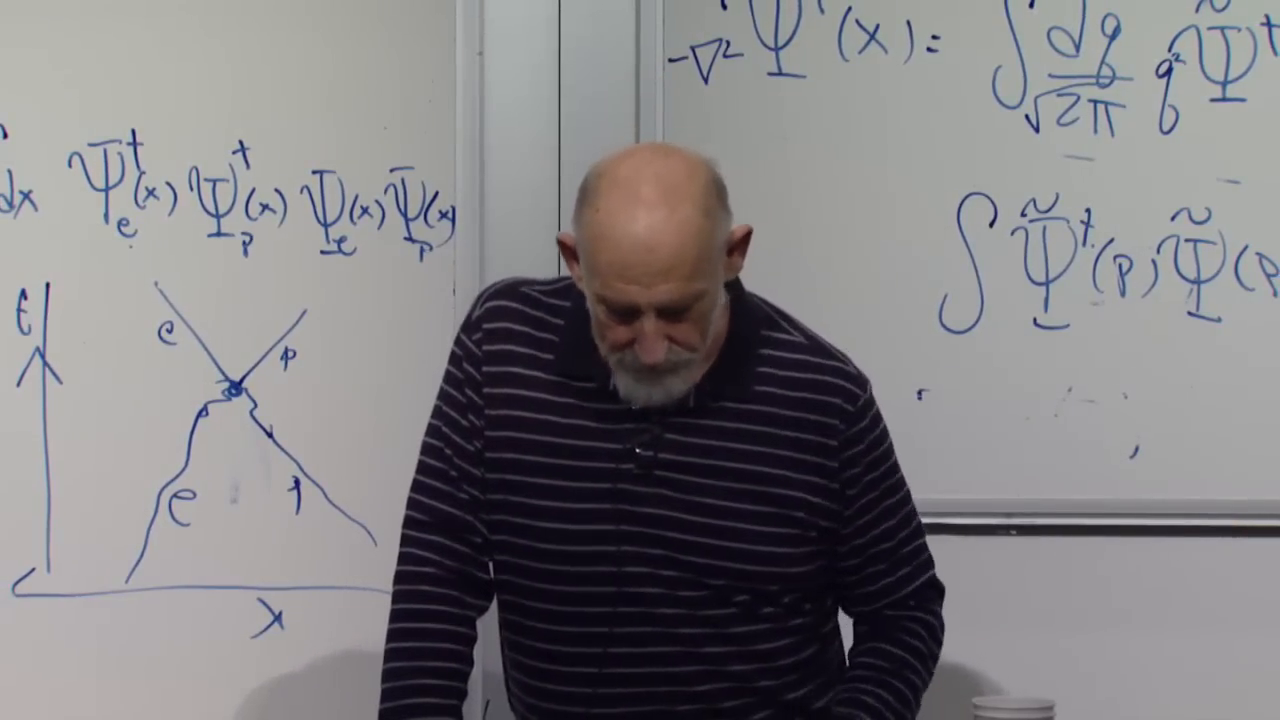
\includegraphics[width=0.94\linewidth]{lecture_09_frame_02.png}
\caption{黑板上的接觸相互作用。時空示意圖上方列出四個局域場算符；這個理想化相互作用只在粒子相遇處作用。}
\lectureframe{00:35:36}
\end{figure}

\begin{figure}[htbp]
\centering
\begin{tikzpicture}[x=1.2cm,y=1.0cm,>=Latex]
\draw[->] (-3.0,0) -- (3.0,0) node[right] {$x$};
\draw[->] (0,-0.2) -- (0,4.2) node[above] {$t$};
\coordinate (v) at (0,2.0);
\fill (v) circle (1.8pt);
\draw[thick,->] (-2.2,0.4) -- (v);
\draw[thick,->] (2.0,0.4) -- (v);
\draw[thick,->] (v) -- (-1.6,3.7);
\draw[thick,->] (v) -- (2.2,3.7);
\node[left] at (-1.65,0.7) {$e$};
\node[right] at (1.55,0.7) {$p$};
\node[left] at (-1.15,3.3) {$e$};
\node[right] at (1.65,3.3) {$p$};
\node[right] at (0.12,2.05) {$g$};
\end{tikzpicture}
\caption{局域散射圖像的清楚重繪。這個頂點是式~\eqref{eq:l9-contact}所示算符的簡寫，不是經典碰撞定律。}
\end{figure}

真實的電子與質子會透過庫侖勢在彼此尚有距離時相互作用。接觸模型只是初步的簡化：如果實驗顯示兩種粒子只有在空間重疊時才會散射，我們就會把類似式~\eqref{eq:l9-contact}的項放進哈密頓量。

\begin{classroomqa}
\lecturetimestamp{00:35:40}
\audiencequestion{如果能量沒有改變，為什麼散射算符會是哈密頓量的一部分？}
\lecturerresponse{哈密頓量既是能量算符，也是產生狀態變化的生成元。兩個粒子之間的勢能會在時間演化中造成散射。總能量守恆，並不表示狀態或個別粒子的動量保持不變。}
\end{classroomqa}

這帶出一條實用原則：先從實驗了解粒子可能經歷哪些局域過程，再用更新狀態的算符將這些過程寫進理論。場的乘積不是純粹裝飾性的代數；其中帶有伴隨符號與不帶伴隨符號的因子，指定了哪些種類的粒子出現或消失。

\section{衰變、逆過程與厄米性}

假設氣泡室中有一條粒子種類\(A\)的徑跡在某點終止，並從該點出現粒子\(B\)與\(C\)的徑跡。這個局域過程是
\begin{equation}
A\longrightarrow B+C.
\end{equation}
實現這個過程的算符是
\begin{equation}
V=g\int dx\,
\psi_B^\dagger(x)\psi_C^\dagger(x)\psi_A(x).
\label{eq:l9-decay-half}
\end{equation}
湮滅場移除\(A\)；兩個產生場則在同一位置產生\(B\)與\(C\)。以相同權重對每個\(x\)積分，便表達了空間平移不變性，並立即得到
\begin{equation}
p_A=p_B+p_C.
\end{equation}

哈密頓量必須是厄米算符。這能確保\(e^{-itH}\)是么正算符，並使總機率保持不變。式~\eqref{eq:l9-decay-half}本身不是厄米的，因此必須再加上它的伴隨項：
\begin{equation}
H_{\mathrm{int}}
=\int dx\left[
g\,\psi_B^\dagger\psi_C^\dagger\psi_A
+g^*\,\psi_A^\dagger\psi_C\psi_B
\right](x).
\label{eq:l9-hermitian-vertex}
\end{equation}
若耦合常數\(g\)為實數，兩項的係數相同。厄米共軛不僅互換帶伴隨符號與不帶伴隨符號的場，也會反轉算符順序。在這個玻色子玩具模型中，不同種類的場彼此對易，因此順序反轉不會造成額外問題。

第二項描述逆過程，
\begin{equation}
B+C\longrightarrow A.
\end{equation}
因此，允許這種衰變的封閉系統么正哈密頓量，也會包含粒子重新結合的振幅。這不代表在任何指定的外部動量下，兩個方向的過程都一定會發生；能量守恆或其他守恆定律可能使其中一個方向在運動學上無法進行。這裡要說的是，該相互作用及其伴隨項都必須納入動力學。

\begin{classroomqa}
\lecturetimestamp{00:42:48}
\audiencequestion{逆過程也會被允許，這項規則有例外嗎？}
\lecturerresponse{就厄米的封閉系統哈密頓量而言，沒有例外：必須包含伴隨相互作用。特定的逆反應仍可能受到運動學條件或其他守恆量子數的阻擋，但其共軛矩陣元素必定存在。}
\end{classroomqa}

數值\(g\)是耦合常數。若\(g\)很小，粒子相遇時的相互作用就很弱；若它很大，躍遷振幅就較大。耦合常數的數值通常由實驗測得，不過對稱性可以約束多個表面上不同的耦合，或將它們彼此聯繫起來。

同樣的語法也能描述更複雜的反應。例如在{\proseunicodefont β}衰變中，
\begin{equation}
n\longrightarrow p+e^-+\bar\nu_e,
\end{equation}
一個示意性的局域項包含四個場：其中一個湮滅中子，另外三個產生質子、電子與電子反微中子；還要加上厄米共軛項，描述逆過程。由此已足以看出，少數幾個算符單項式便開始構成一套量子場論。

\section{為什麼哈密頓量的平方如此重要}

短時間演化公式\eqref{eq:l9-short-update}只保留到\(\epsilon\)的一階。完整的展開式是
\begin{equation}
e^{-i\epsilon H}
=1-i\epsilon H-\frac{\epsilon^2}{2}H^2
+\frac{i\epsilon^3}{3!}H^3+\cdots.
\label{eq:l9-exponential}
\end{equation}
在二階項中，哈密頓量作用兩次。第一批複合過程圖像的代數根源就在這裡。

對於頂點\(A\leftrightarrow B+C\)，第一次作用可以讓\(B+C\)結合成\(A\)；第二次作用則能使這個\(A\)再分解成\(B+C\)：
\begin{equation}
B+C\longrightarrow A\longrightarrow B+C.
\label{eq:l9-bc-scattering}
\end{equation}
總貢獻是\(B+C\to B+C\)的散射振幅。中間的\(A\)並不是另一個可觀測事件，而是標示兩次相互作用之間所求和的中間態。

\begin{classroomqa}
\lecturetimestamp{00:49:54}
\audiencequestion{寫出的二階乘積中，\(C\)場是否應該帶有伴隨符號？}
\lecturerresponse{是的，算符順序必須符合所描述的過程。第一個頂點湮滅\(B\)和\(C\)，並產生\(A\)；第二個頂點湮滅\(A\)，再產生\(B\)和\(C\)。只要正確寫出相應的伴隨符號，算符就會符合這個過程。}
\end{classroomqa}

\begin{figure}[htbp]
\centering
\includegraphics[width=0.94\linewidth]{lecture_09_frame_05.png}
\caption{黑板上基本頂點\(A\leftrightarrow B+C\)的兩種方向。將它們並列，是式~\eqref{eq:l9-bc-scattering}所示二階過程的圖像簡記。}
\lectureframe{00:48:56}
\end{figure}

現在再加入一個旁觀粒子\(B\)。第一次作用使\(A\)發射\(C\)，並轉變為\(B\)；稍後，該\(C\)與原先的\(B\)結合，形成\(A\)。外部粒子仍是\(A+B\)，但動量可以改變。這個過程可描述為\(A\)與\(B\)透過交換\(C\)而散射。

\begin{figure}[htbp]
\centering
\includegraphics[width=0.94\linewidth]{lecture_09_frame_06.png}
\caption{黑板上的交換過程。右側圖以一條內部\(C\)線連接兩個基本頂點，同時外部的\(A\)與\(B\)粒子發生散射。}
\lectureframe{00:51:22}
\end{figure}

\begin{figure}[htbp]
\centering
\begin{tikzpicture}[x=1.1cm,y=1cm,>=Latex]
\draw[->] (-3.7,-0.2) -- (-3.7,4.2) node[above] {$t$};
\coordinate (v1) at (-0.9,1.25);
\coordinate (v2) at (0.9,2.95);
\fill (v1) circle (1.7pt);
\fill (v2) circle (1.7pt);
\draw[thick,->] (-2.6,0.2) -- (v1) node[midway,below left] {$A$};
\draw[thick,->] (2.6,0.2) -- (v2) node[midway,below right] {$B$};
\draw[thick,->] (v1) -- (-2.4,4.0) node[midway,left] {$B$};
\draw[thick,->] (v2) -- (2.5,4.0) node[midway,right] {$A$};
\draw[thick,->,dashed] (v1) -- (v2) node[midway,above left] {$C$};
\node[below] at (0,-0.05) {$A+B\rightarrow A+B$};
\end{tikzpicture}
\caption{\(C\)交換過程的清楚重繪。每個頂點都貢獻一個\(g\)因子，因此這個二階項正比於\(g^2\)。}
\end{figure}

每一個局域相互作用點稱為一個頂點。每個頂點都貢獻一個耦合常數因子，因此兩個頂點的貢獻帶有\(g^2\)，三個頂點的貢獻帶有\(g^3\)，依此類推。因此，哈密頓量中的單一項就能將一大類反應聯繫起來。這種簡潔性是量子場論強大之處：少數幾種局域相互作用，就能組織起大量散射資料。

\begin{classroomqa}
\lecturetimestamp{00:53:14}
\audiencequestion{過程\(A\to B+C\to A\)稱為什麼？}
\lecturerresponse{這是自能貢獻。測得的\(A\)不只是裸的單粒子基底態；相互作用態也包含鄰近的\(B+C\)分量，並具有相應的振幅。對這個態進行散射，可以揭示其著裝結構。}
\end{classroomqa}

量子電動力學提供了一個熟悉的例子。在局域的電子--光子頂點，電子可以被湮滅後再產生，並同時產生一個光子。在二階過程中，電子可能發射並重新吸收光子。人們很容易把這個過程講成一段微型電影，但嚴謹地說，它只是微擾展開中的一項。物理電子是一個著裝態，其中包含光子成分。

課堂上估計這個成分``約為百分之一''，是要傳達精細結構常數\(\alpha_{\mathrm{em}}\simeq 1/137\)所設定的量級。光子福克態成分的精確機率，取決於能量解析度以及相互作用態的定義方式；孤立電子並不普遍具有恰好百分之一的這項性質。可靠的結論是，相互作用會改變電子可測量的結構。

\section{圖形能說明什麼，不能說明什麼}

這些圖形是計算相互作用哈密頓量各次方的簡記，不能當成可靠的經典歷史，彷彿粒子確定先發生一個事件，再發生另一個事件。若深入探究並判定哪一個中間可能性``真的發生了''，就會改變實驗並破壞相干求和，情況如同一般的量子干涉。

\begin{classroomqa}
\lecturetimestamp{00:56:52}
\audiencequestion{第一個頂點處的能量和動量都守恆嗎？}
\lecturerresponse{在這裡採用的等時哈密頓量架構中，空間積分會立即產生動量{\proseunicodefont δ}函數。對於單獨這一次相互作用插入，尚未進行時間積分，因此不會產生能量{\proseunicodefont δ}函數。完整且具有時間平移不變性的散射振幅會守恆總能量；中間線則不必符合可觀測粒子的在殼關係。在協變圖的語言中，每個頂點處的四動量守恆，但內部粒子可以是離殼的。}
\end{classroomqa}

在直觀的頂點圖像中，能量似乎不見了；這再次提醒我們，不要忽略相互作用能。總哈密頓量不只是自由粒子能量的總和。若遇到疑問，就回到式~\eqref{eq:l9-exponential}：這個圖形代表么正時間演化展開式中的一項。完整的費曼圖方法會系統地處理時間排序、傳播子、積分與對稱因子，但基本物理從這裡開始。

有個延伸問題把圖形理解得過於字面，將發射出的光子與緩慢運動電子周圍的電場相提並論。

\begin{classroomqa}
\lecturetimestamp{00:58:26}
\audiencequestion{電子在一段距離外的電場，真的是由輻射光子產生的嗎？這和干涉以及阿哈羅諾夫--玻姆效應如何相容？}
\lecturerresponse{靜電場或感應場並不是由真實輻射光子構成的流。量子電動力學以同一個場描述輻射與電子的電磁著裝，但相應的量子態和運動學條件並不相同。對極端相對論性的電子而言，某些場分量可以近似視為近乎真實光子的通量；對緩慢運動的電子而言，把光子想成沿著明確軌跡移動並不恰當。雙縫干涉與阿哈羅諾夫--玻姆效應也是非經典的場現象，但它們並不會使這個自能圖變成一段機械式的電影。}
\end{classroomqa}

\begin{classroomqa}
\lecturetimestamp{01:01:28}
\audiencequestion{經典圖像究竟為什麼會失效？}
\lecturerresponse{因為計算會將所有可能的中間過程振幅相干地相加。經驗有助於我們直觀地理解這些圖像，但它們在字面上所能表達的，始終不超出定義它們的算符展開。這些圖像是計算\(H^2,H^3,\ldots\)的簡潔方式，並不是對已觀測中間事件的記錄。}
\end{classroomqa}

\begin{classroomqa}
\lecturetimestamp{01:03:04}
\audiencequestion{一般的庫侖相互作用能否從光子交換的古典極限中導出？}
\lecturerresponse{可以。計算適當的光子媒介振幅，再取其非相對論靜態極限，就會得到庫侖勢。這項推導比目前的算符示意圖更為複雜，但仍不應將它理解成光子真的在兩個古典粒子之間跳來跳去。}
\end{classroomqa}

\begin{classroomqa}
\lecturetimestamp{01:03:44}
\audiencequestion{耦合常數是從場的乘積計算出來的嗎？}
\lecturerresponse{通常，耦合常數的數值是由實驗提供的輸入。對稱性可以限制其取值，或將原本彼此獨立的耦合聯繫起來。如果這樣的關係預測了不同反應的相對強度，而且得到實驗證實，這項符合就格外具有啟發性。}
\end{classroomqa}

\begin{classroomqa}
\lecturetimestamp{01:04:48}
\audiencequestion{偶然對稱性與規範對稱性各自扮演什麼角色？}
\lecturerresponse{規範對稱性會直接限制允許的結構，以及耦合常數之間的關係。偶然對稱性並未在基本層次上被強加；它之所以出現，是因為所有允許的低階相互作用恰好都尊重這項對稱性。它仍可能帶來重要後果，但其起源與穩健性都不同於規範對稱性。}
\end{classroomqa}

非相對論場論目前先講到這裡。我們先前說過要談費米子。與其立刻對費米子進行二次量子化，不如先了解它們的場算符必須滿足的相對論性單粒子方程。

\section{電子為何需要相對論}

先從一維空間開始。這不是對真實情況的合理限制，但能去除三維自旋的幾何複雜性，同時保留核心代數結構。電子的質量很小，因此即使在原子中，相對論效應也很重要。在氫原子中，電子的典型速度量級為
\begin{equation}
v\sim\alpha_{\mathrm{em}}c\approx 0.007c,
\end{equation}
約為光速的百分之一。對重原子中的內層電子而言，粗略的速度尺度則變為\(v\sim Z\alpha_{\mathrm{em}}c\)，因此相對論修正可能相當顯著。無論決定性的動機來自歷史上的好奇心，還是對原子物理精度的要求，相對論性的Schr\"odinger類方程在物理上都是必要的。

通常的量子化步驟從能量與動量之間的古典關係出發。非相對論情況下，
\begin{equation}
E=\frac{p^2}{2m},
\end{equation}
作以下代換
\begin{equation}
E\mapsto i\partial_t,
\qquad
p\mapsto-i\partial_x
\end{equation}
便得到
\begin{equation}
i\partial_t\varphi(x,t)
=-\frac{1}{2m}\partial_x^2\varphi(x,t).
\end{equation}

相對論則給出以下關係，並取\(c=1\)：
\begin{equation}
E^2=p^2+m^2.
\label{eq:l9-rel-dispersion}
\end{equation}

\begin{figure}[htbp]
\centering
\includegraphics[width=0.94\linewidth]{lecture_09_frame_07.png}
\caption{黑板上從\(E=p^2/2m\)轉向相對論關係式\(E^2=p^2+m^2\)，其中\(c=1\)。}
\lectureframe{01:10:30}
\end{figure}

將這些代換代入平方後的關係式，得到
\begin{equation}
-\partial_t^2\varphi
=\left(-\partial_x^2+m^2\right)\varphi,
\label{eq:l9-klein-gordon}
\end{equation}
也可以寫成
\begin{equation}
\left(\partial_t^2-\partial_x^2+m^2\right)\varphi=0.
\end{equation}
這就是克萊因--戈登方程。這是一個有明確意義的相對論性場方程，尤其適用於自旋為零的場。但我們所要的電子方程必須對時間為一階，
\begin{equation}
i\partial_t\Psi=H\Psi,
\end{equation}
使\(H\)本身，而非只有\(H^2\)，就能產生時間演化。

形式上，我們可以令
\begin{equation}
H=\sqrt{-\partial_x^2+m^2}.
\end{equation}
這個平方根在動量空間中能明確定義，此時它乘上\(\sqrt{p^2+m^2}\)；但在位置空間中，它是非局域的偽微分算符。這在技術上行得通，卻不利於我們尋找局域方程的目標。因此我們重新出發。

\section{無質量右行波}

先考慮一個向右運動的無質量粒子。它的正能量與動量滿足
\begin{equation}
E=p
\qquad (c=1).
\end{equation}
量子化後得到
\begin{equation}
i\partial_t\psi=-i\partial_x\psi,
\end{equation}
亦即
\begin{equation}
(\partial_t+\partial_x)\psi=0.
\label{eq:l9-right-mover}
\end{equation}
所有解的形式都是
\begin{equation}
\psi(x,t)=f(x-t).
\end{equation}
波形保持不變，並以光速向右傳播。

立刻會遇到兩個問題。第一，若讓式~\eqref{eq:l9-right-mover}作用於任意傅立葉模式，負動量的能量就是\(E=p<0\)，因此哈密頓量沒有下界。若逕自限制\(p>0\)，便只留下右行波；這還不是我們要的電子理論。第二，這個方程只能描述一個方向，沒有一般的左行電子。我們先處理左右行的問題，並暫時保留負能量的問題。

\section{兩個分量與阿爾法矩陣}

引入兩個振幅，
\begin{equation}
\Psi(x,t)=
\begin{pmatrix}
\psi_1(x,t)\\[3pt]
\psi_2(x,t)
\end{pmatrix},
\end{equation}
在無質量極限下，\(\psi_1\)是右行分量，\(\psi_2\)是左行分量：
\begin{align}
(\partial_t+\partial_x)\psi_1&=0,
&
(\partial_t-\partial_x)\psi_2&=0.
\end{align}
量子力學也允許兩者任意相干疊加。因此，粒子可以同時具有向兩個方向運動的振幅，而不必像古典粒子那樣從一開始就固定選定一個方向。

這個額外的二值自由度在代數上類似自旋，但在一維中並不是通常的角動量。定義
\begin{equation}
\alpha=
\begin{pmatrix}
1&0\\
0&-1
\end{pmatrix}
=\sigma_3.
\label{eq:l9-alpha}
\end{equation}
其 \(+1\) 本徵向量選出右行分量，其 \(-1\) 本徵向量則選出左行分量。在無質量理論中，哈密頓量就是
\begin{equation}
H=\alpha p,
\end{equation}
而兩個方程可合併為
\begin{equation}
i\partial_t\Psi=-i\alpha\partial_x\Psi.
\label{eq:l9-massless-dirac}
\end{equation}

\begin{classroomqa}
\lecturetimestamp{01:22:44}
\audiencequestion{區分這兩個分量的對角矩陣叫什麼？}
\lecturerresponse{作為泡利矩陣，它是 \(\sigma_3\)，不是 \(\sigma_1\)。在狄拉克對此處構造所採用的記號中，我們稱它為 \(\alpha\)。它遵循熟悉的泡利代數，儘管這裡的物理標籤代表方向，而非自旋角動量。}
\end{classroomqa}

\begin{classroomqa}
\lecturetimestamp{01:23:32}
\audiencequestion{在三維中，方向是向量，這個構造是否會有更幾何的意義？}
\lecturerresponse{會。三維問題需要為每個空間方向配置一個矩陣，並導向更豐富的旋量結構。儘管如此，一維模型在其適用範圍內仍是精確的，而且能在不引入那些額外複雜性的情況下，單獨呈現左右方向的核心代數。}
\end{classroomqa}

\begin{figure}[htbp]
\centering
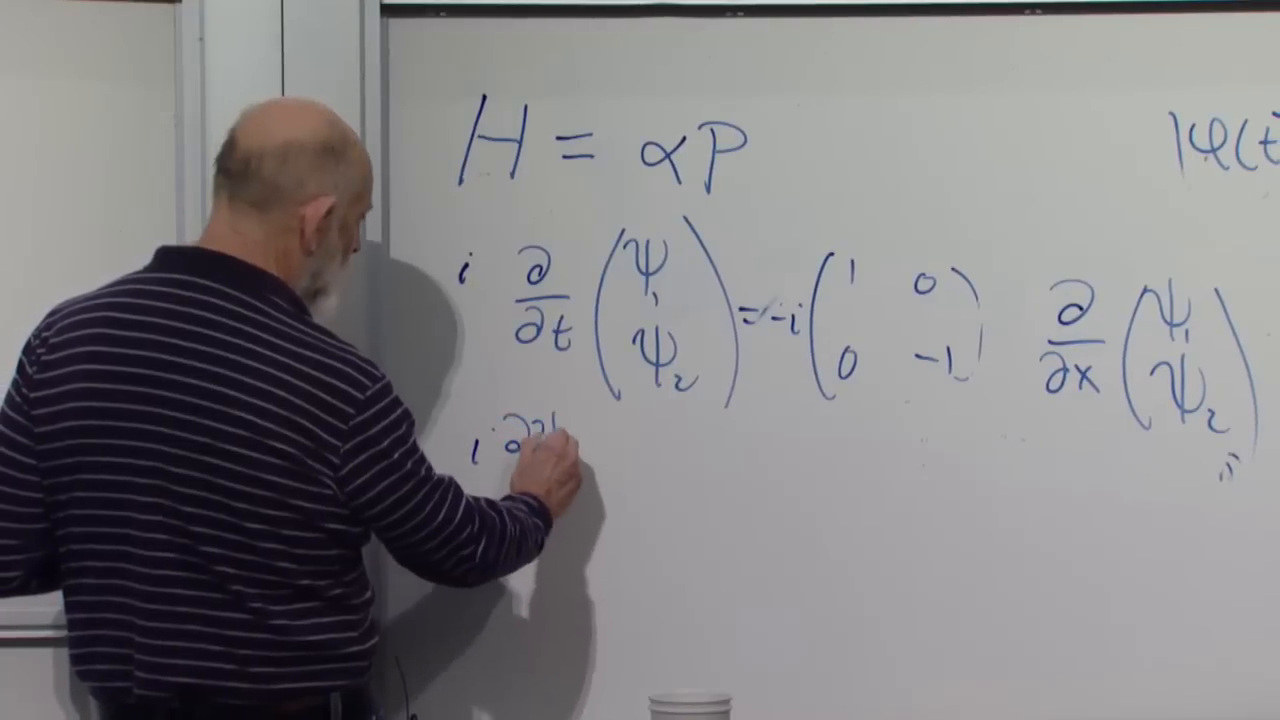
\includegraphics[width=0.94\linewidth]{lecture_09_frame_03.png}
\caption{黑板上的無質量二分量方程：\(H=\alpha P\)；對角矩陣為 \(\psi_1\) 和 \(\psi_2\) 指定相反的傳播方向。}
\lectureframe{01:26:00}
\end{figure}

單向傳播的問題解決了。負能量譜依然存在，而且我們又發現了第三個缺陷：兩個分量仍然沒有質量，並以光速傳播。接下來必須引入靜止能量，並將兩個方向耦合起來。

\section{加入質量並發現狄拉克代數}

加入一個最一般的簡單質量正比項，
\begin{equation}
H=\alpha p+\beta m,
\label{eq:l9-dirac-hamiltonian}
\end{equation}
其中 \(\beta\) 只作用於二分量指標。它可以是單位矩陣，也可以是其他矩陣；由相對論性色散關係來決定。

由於 \(H^2\) 必須等於 \(p^2+m^2\)，將式~\eqref{eq:l9-dirac-hamiltonian}平方：
\begin{align}
H^2
&=(\alpha p+\beta m)^2\\
&=\alpha^2p^2+\beta^2m^2
+(\alpha\beta+\beta\alpha)pm.
\label{eq:l9-square-dirac}
\end{align}
這些矩陣與 \(p\) 對易，因為它們作用於內部的二分量空間，而 \(p\) 作用於空間波函數。要符合式~\eqref{eq:l9-rel-dispersion}，必須滿足
\begin{equation}
\alpha^2=\mathbb{1},
\qquad
\beta^2=\mathbb{1},
\qquad
\{\alpha,\beta\}
=\alpha\beta+\beta\alpha=0.
\label{eq:l9-dirac-algebra}
\end{equation}
對 \(\alpha=\sigma_3\) 而言，第一個條件已經成立。任何不同的泡利矩陣都與它反對易，而且平方為單位矩陣。選擇
\begin{equation}
\beta=
\begin{pmatrix}
0&1\\
1&0
\end{pmatrix}
=\sigma_1.
\label{eq:l9-beta}
\end{equation}
選 \(\sigma_1\) 而不選 \(\sigma_2\) 是基底慣例；經過么正基底變換後，兩者實現的是相同的代數。

\begin{classroomqa}
\lecturetimestamp{01:33:00}
\audiencequestion{狄拉克只是看出泡利矩陣滿足這些代數條件嗎？}
\lecturerresponse{歷史上的推導是在三維中直接進行，並引入滿足所需關係的矩陣。寫出這些條件後，利用泡利代數便能立即得到一維解：選取兩個不同的泡利矩陣。}
\end{classroomqa}

\begin{classroomqa}
\lecturetimestamp{01:34:24}
\audiencequestion{這個 \(\beta\) 是相對論中的速度參數 \(v/c\) 嗎？}
\lecturerresponse{不是。它是作用於旋量分量的矩陣。字母重複使用只是狄拉克的記號，與運動學量 \(v/c\) 無關。}
\end{classroomqa}

在三個空間維度中，\(2\times2\) 矩陣不足以構成所需反對易矩陣的完整集合。這部分留待之後處理。在一維中，式~\eqref{eq:l9-alpha}和\eqref{eq:l9-beta}已經足夠。

\section{耦合的一維狄拉克方程}

代入 \(p=-i\partial_x\)，得到哈密頓形式的一維狄拉克方程：
\begin{equation}
i\partial_t\Psi
=\left(-i\alpha\partial_x+\beta m\right)\Psi.
\label{eq:l9-one-dimensional-dirac}
\end{equation}
由於 \(\alpha\) 是對角矩陣，導數項會讓兩個分量各自保持分離；由於 \(\beta\) 是非對角矩陣，質量項會使兩個分量互相轉換。逐分量寫成
\begin{align}
i\partial_t\psi_1
&=-i\partial_x\psi_1+m\psi_2,
\label{eq:l9-dirac-component-one}\\
i\partial_t\psi_2
&=+i\partial_x\psi_2+m\psi_1.
\label{eq:l9-dirac-component-two}
\end{align}

\begin{figure}[htbp]
\centering
\includegraphics[width=0.94\linewidth]{lecture_09_frame_08.png}
\caption{黑板上的耦合分量方程。導數項中相反的符號代表右行與左行；非對角的質量項則使 \(\psi_1\) 和 \(\psi_2\) 互相轉換。}
\lectureframe{01:37:44}
\end{figure}

只要 \(m\ne0\)，兩個分量就不再獨立演化。將一階方程平方後，每個分量都會得到克萊因--戈登算符：
\begin{equation}
\left(\partial_t^2-\partial_x^2+m^2\right)\psi_a=0,
\qquad a=1,2,
\end{equation}
平面波滿足 \(E^2=p^2+m^2\)，其群速度為
\begin{equation}
v_g=\frac{dE}{dp}=\frac{p}{E},
\end{equation}
只要質量不為零，群速度的大小就小於一。

質量與左右混合之間的關係並非偶然。無質量的右行粒子在任何正向洛倫茲變換下都仍是右行粒子；亞光速觀察者無法超越光，也就無法反轉它的方向。有質量的粒子可以被帶到靜止，再從沿同一方向運動且速度更快的參考系觀察；在該參考系中，粒子的速度看起來會反向。因此，有質量的相對論理論不可能讓右行與左行扇區永遠彼此隔離。非對角質量項恰好提供所需的耦合。

\begin{classroomqa}
\lecturetimestamp{01:40:01}
\audiencequestion{兩個分量互相轉換，這算是手徵振盪嗎？}
\lecturerresponse{在這個一維基底中，\(\alpha\)區分兩個無質量的手徵方向。質量項是非對角的，會使兩者混合，因此手徵性不再守恆。就此而言，質量項是手徵振盪的來源。}
\end{classroomqa}

\begin{classroomqa}
\lecturetimestamp{01:40:46}
\audiencequestion{為什麼費米子方程應該是玻色子方程的平方根？}
\lecturerresponse{不應該這樣理解。色散關係 \(E^2=p^2+m^2\) 適用於所有自由相對論粒子，不受統計性質影響。狄拉克算符恰好提供克萊因--戈登算符的矩陣分解，但這種代數關係並不能從玻色子推導出費米子。}
\end{classroomqa}

\begin{classroomqa}
\lecturetimestamp{01:41:31}
\audiencequestion{能否將方程化為簡單的純量分解，分別得到左行與右行因子？}
\lecturerresponse{只有在無質量極限下，兩個手徵方程才會解耦，成為彼此獨立的純量因子。當 \(m\ne0\) 時，有用的分解是矩陣值分解：反對易的 \(\alpha\) 與 \(\beta\) 矩陣正是消去多餘交叉項的關鍵。}
\end{classroomqa}

\begin{classroomqa}
\lecturetimestamp{01:42:04}
\audiencequestion{這兩個耦合方程已經構成狄拉克方程了嗎？}
\lecturerresponse{是的。兩式合起來就是一維空間中的狄拉克方程，也可以寫成式~\eqref{eq:l9-one-dimensional-dirac}的緊湊形式。乘上 \(\beta\) 可得到更對稱的協變記法，但這種寫法留待之後討論。}
\end{classroomqa}

還有兩項工作刻意留待後續處理。這個構造沒有消除負能量；它在兩個方向扇區中都提供了負能量解，因此這個問題反而更為明顯。而且理論仍然局限於一個空間維度。接下來要解釋負能量解，並將矩陣代數擴充到 \(3+1\) 維。

\chapter{費米子、狄拉克矩陣與狄拉克海}

狄拉克海是我們要探討的終點，但抵達的路徑也很重要。在處理相對論性電子理論中的負能量之前，我們需要先掌握兩項工具。首先是用來區分費米子與玻色子的算符代數；接著回顧一維狄拉克方程，藉此不必借助三維空間幾何，就能清楚看出波函數的每一次擴充。掌握這些之後，三維方程便會要求我們採用相應的矩陣結構；而開頭談到的費米子態填滿與空缺，則會再次成為理解正電子的關鍵。

我們採用\(c=\hbar=1\)。大寫\(P\)表示動量算符，小寫\(p\)表示動量本徵值，粗體符號則表示它們的三維版本。

\section{交換如何化為算符代數}

考慮兩個全同粒子，一個位於\(x\)，另一個位於\(y\)。標記\(x\)和\(y\)表示完整的位置，並非單一粒子的兩個笛卡兒座標。以兩個產生算符作用於真空，得到
\begin{equation}
\lvert x,y\rangle
=
\psi^\dagger(x)\psi^\dagger(y)\lvert0\rangle.
\label{eq:l10-two-particle-state}
\end{equation}

對玻色子而言，交換這兩個位置不會改變量子態：
\begin{equation}
\lvert x,y\rangle=\lvert y,x\rangle.
\end{equation}
確保這種對稱性的算符關係是
\begin{equation}
\psi^\dagger(x)\psi^\dagger(y)
=
\psi^\dagger(y)\psi^\dagger(x).
\label{eq:l10-boson-exchange}
\end{equation}
兩個玻色子產生算符彼此對易，因此交換它們的順序，不會改變所產生的量子態。

對費米子而言，交換會使符號反轉：
\begin{equation}
\lvert x,y\rangle=-\lvert y,x\rangle.
\label{eq:l10-fermion-state-exchange}
\end{equation}
單一態向量的整體符號無法觀測，但不同可能性之間的相對符號可以觀測，因此必須一致地保留這個負號。式~\eqref{eq:l10-fermion-state-exchange}要求
\begin{equation}
\psi^\dagger(x)\psi^\dagger(y)
=
-\,\psi^\dagger(y)\psi^\dagger(x).
\label{eq:l10-fermion-operator-exchange}
\end{equation}

\begin{figure}[htbp]
\centering
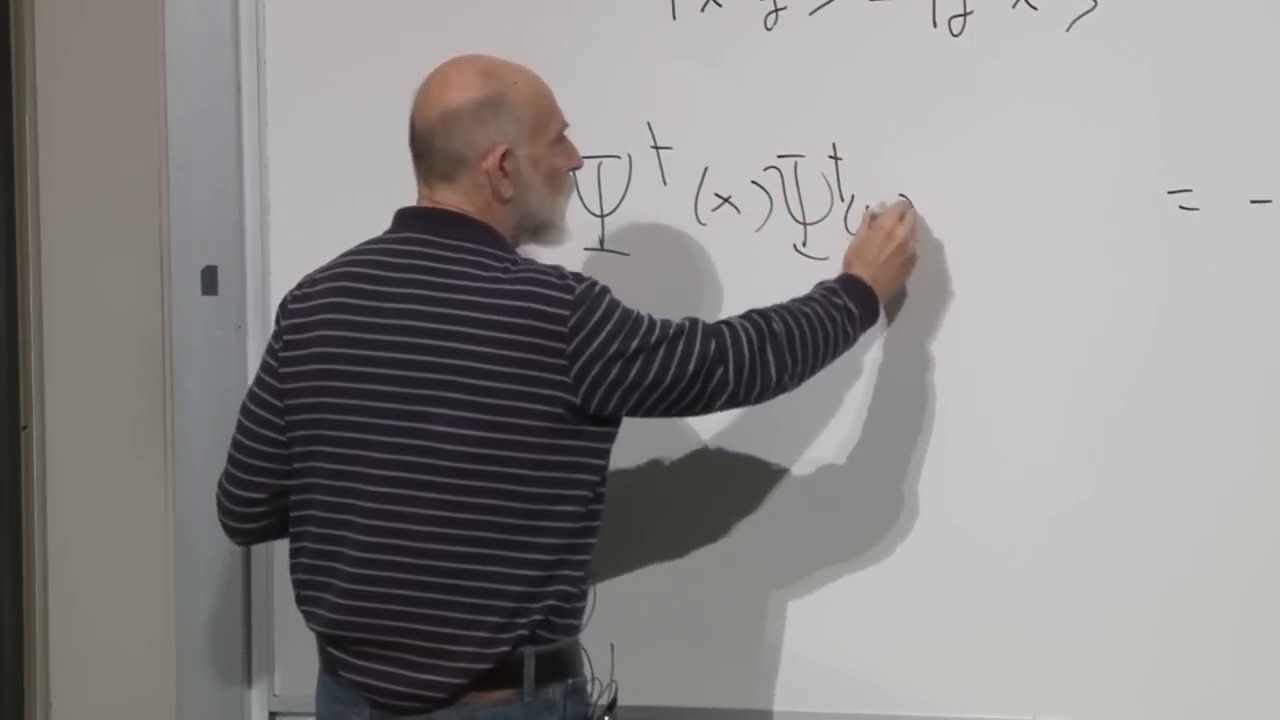
\includegraphics[width=0.94\linewidth]{lecture_10_figure_02.png}
\caption{黑板上表示費米子交換的關係。交換產生算符的順序，會使兩粒子態的符號反轉。}
\lectureframe{00:05:50}
\end{figure}

對任意兩個算符\(A\)和\(B\)，反對易子定義為
\begin{equation}
\{A,B\}:=AB+BA.
\end{equation}
因此，交換規則是
\begin{equation}
\{\psi^\dagger(x),\psi^\dagger(y)\}=0.
\label{eq:l10-creation-anticommutator}
\end{equation}
相應的費米子場代數以反對易子取代玻色子場的對易子。這裡必須區分「反對易」一詞的兩種用法：場算符因費米統計而反對易；稍後矩陣彼此反對易，則是為了消去相對論性色散關係中的交叉項。

現在在式~\eqref{eq:l10-creation-anticommutator}中令\(y=x\)。兩個乘積便相同：
\begin{align}
0
&=\{\psi^\dagger(x),\psi^\dagger(x)\}\\
&=2\,\psi^\dagger(x)\psi^\dagger(x).
\end{align}
因此
\begin{equation}
\bigl(\psi^\dagger(x)\bigr)^2=0.
\label{eq:l10-exclusion}
\end{equation}
若試圖在同一單粒子態中產生兩個相同的費米子，結果會是零向量。這就是排他原理的算符形式。

\begin{figure}[htbp]
\centering
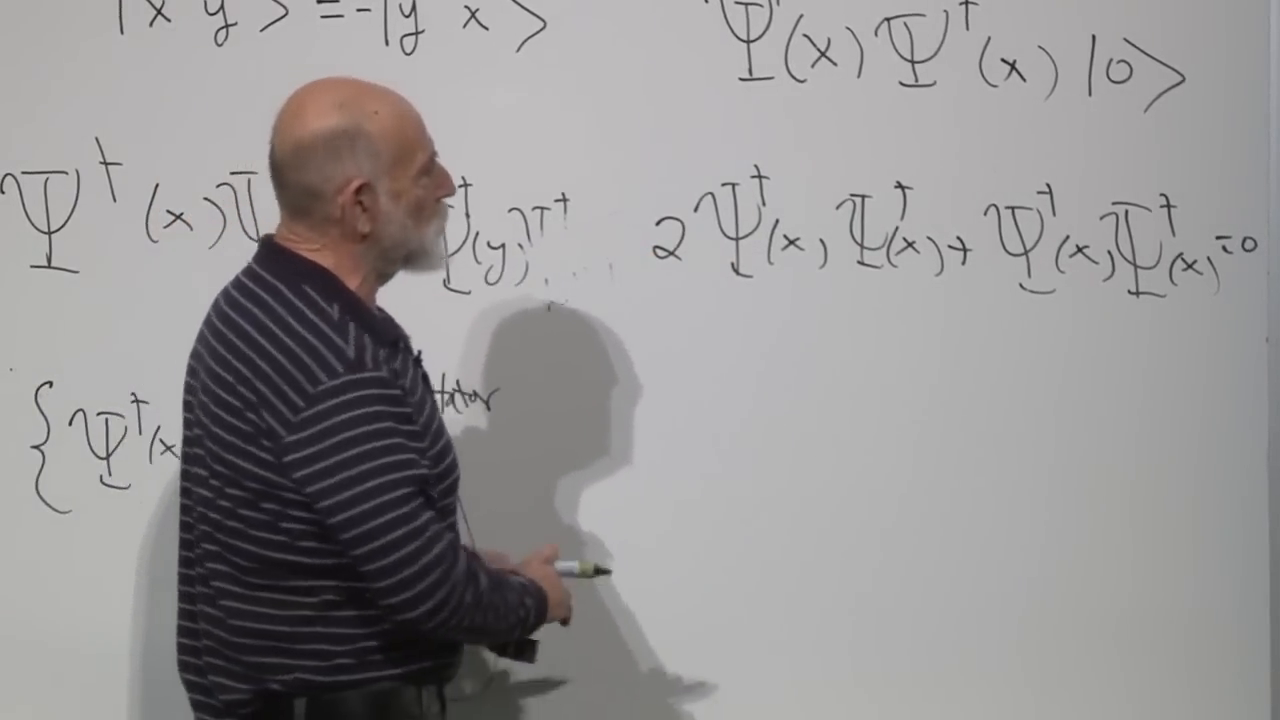
\includegraphics[width=0.94\linewidth]{lecture_10_figure_03.png}
\caption{黑板上將兩態取為相同態的情形。重複的產生算符乘積出現兩次，因此必須為零。}
\lectureframe{00:08:04}
\end{figure}

\begin{figure}[htbp]
\centering
\begin{adjustbox}{max width=\linewidth}
\begin{tikzpicture}[node distance=1.25cm,>=Latex]
\node[draw,rounded corners,align=center,inner sep=7pt] (a)
  {$\{\psi^\dagger(x),\psi^\dagger(x)\}=0$};
\node[draw,rounded corners,align=center,inner sep=7pt,right=of a] (b)
  {$2(\psi^\dagger(x))^2=0$};
\node[draw,rounded corners,align=center,inner sep=7pt,right=of b] (c)
  {$(\psi^\dagger(x))^2=0$};
\draw[->,thick] (a) -- (b);
\draw[->,thick] (b) -- (c);
\end{tikzpicture}
\end{adjustbox}
\caption{不依賴黑板上已部分擦除的中間推導，重新呈現排他原理的論證。}
\end{figure}

\section{為什麼費米子的填滿態與空態具有對稱性}

玻色子與費米子算符之間還有第二個差異，這個差異比排他原理更微妙，對後續內容也至關重要。對單一玻色子模態而言，
\begin{equation}
[a,a^\dagger]=1,
\qquad
n=0,1,2,\ldots.
\end{equation}
交換\(a\)與\(a^\dagger\)，會使對易子的符號反轉。即使只把這些算符稱作\(A\)和\(B\)，代數仍會指出哪種排列會增加佔據數，哪種會減少佔據數。

玻色子的佔據階梯也有方向。湮滅算符最終會到達\(\lvert0\rangle\)，並將它化為零；產生算符則可以不斷繼續作用：
\begin{align}
a\lvert0\rangle&=0,\\
a^\dagger\lvert n\rangle&\propto\lvert n+1\rangle,
\qquad n=0,1,2,\ldots.
\end{align}
將這個階梯上下顛倒，並不會得到相同的能譜。它有底端，卻沒有頂端。

對單一費米子模態而言，
\begin{equation}
\{a,a^\dagger\}=1,
\qquad
a^2=(a^\dagger)^2=0,
\qquad
n=0,1.
\label{eq:l10-fermion-mode}
\end{equation}
產生算符將空態變為滿態，之後便停止作用：
\begin{equation}
a^\dagger\lvert0\rangle=\lvert1\rangle,
\qquad
a^\dagger\lvert1\rangle=0.
\end{equation}
湮滅算符則執行相反的操作：
\begin{equation}
a\lvert1\rangle=\lvert0\rangle,
\qquad
a\lvert0\rangle=0.
\end{equation}
只有兩種態，因此交換滿態與空態，並交換\(a\)與\(a^\dagger\)，圖示仍保持對稱。這兩個算符的物理意義仍然不同，但它們的代數不再特別指定其中一個為產生算符、另一個為湮滅算符。這種形式上的對稱性，正是粒子—空穴重新詮釋的起點。

\begin{classroomqa}
\lecturetimestamp{00:13:54}
\audiencequestion{如果\((a^\dagger)^2=0\)，這是矛盾嗎？還是表示\(a^\dagger=0\)？}
\lecturerresponse{兩者皆非。非零算符的平方可以為零。這裡，\(a^\dagger\)將\(\lvert0\rangle\)變為\(\lvert1\rangle\)，但\(\lvert1\rangle\)之上沒有可允許的態，因此對它作用兩次，結果為零。同理可得\(a^2=0\)。}
\end{classroomqa}

先記住這種滿態與空態之間的對稱性。移除一個負能量電子時，湮滅算符會重新標記為正電子產生算符。這不是任意更改符號，而是運用了此處建立的兩態費米子代數。

\section{一維狄拉克方程的構造}

現在回到一維空間中的單一粒子。最簡單的一階相對論性波動方程是
\begin{equation}
i\partial_t\psi=-\,i\partial_x\psi.
\label{eq:l10-right-mover}
\end{equation}
取\(P=-i\partial_x\)後，方程成為
\begin{equation}
H=P.
\end{equation}
動量本徵態滿足\(E=p\)，其群速度為
\begin{equation}
v_g=\frac{dE}{dp}=1.
\end{equation}
動量為正或為負，因而能量為正或為負，波仍都以固定形狀向右傳播。\(p\)的符號會改變相位的分布，而非傳播方向。

有質量的粒子必須能向任一方向運動。引入第二個分量，使其滿足
\begin{equation}
H\psi_1=P\psi_1,
\qquad
H\psi_2=-P\psi_2.
\label{eq:l10-two-directions}
\end{equation}
第一個分量向右傳播，第二個分量向左傳播。將兩者排成一個欄向量，
\begin{equation}
\Psi=
\begin{pmatrix}
\psi_1\\
\psi_2
\end{pmatrix},
\end{equation}
並定義
\begin{equation}
\alpha=
\begin{pmatrix}
1&0\\
0&-1
\end{pmatrix}.
\end{equation}
兩個方程便都可以寫成
\begin{equation}
H\Psi=\alpha P\Psi.
\label{eq:l10-massless-one-d}
\end{equation}
納入兩個傳播方向，代價是引入一個新的二值內部自由度。

只有傳播方向還不足以產生質量。引入第二個矩陣，
\begin{equation}
\beta=
\begin{pmatrix}
0&1\\
1&0
\end{pmatrix},
\end{equation}
並令哈密頓量為
\begin{equation}
H=\alpha P+\beta m.
\label{eq:l10-massive-one-d}
\end{equation}
這些矩陣滿足
\begin{equation}
\alpha^2=\beta^2=\mathbb{1},
\qquad
\{\alpha,\beta\}=0.
\label{eq:l10-one-d-algebra}
\end{equation}
將哈密頓量平方，得到
\begin{align}
H^2
&=(\alpha P+\beta m)^2\\
&=\alpha^2P^2+\beta^2m^2
  +(\alpha\beta+\beta\alpha)Pm\\
&=P^2+m^2.
\label{eq:l10-one-d-dispersion}
\end{align}
式~\eqref{eq:l10-one-d-algebra}中的反對易子會消去同時含有\(P\)與\(m\)的多餘項。

非對角矩陣\(\beta\)將兩個方向分量耦合起來。可以把質量項想成持續混合向右與向左傳播的振幅。這個圖像不應被理解成粒子真的沿著微觀軌道來回彈跳，但它說明了為何有質量波包的平均速度可以低於光速，也說明了為何它可以有靜止參考系，而孤立的無質量手徵分量則不能。

\begin{classroomqa}
\lecturetimestamp{00:23:37}
\audiencequestion{引入兩個方向分量，是否有更深一層的物理解釋？}
\lecturerresponse{有，不過到了三維時，這種解釋會更清楚。目前這兩個分量只是描述相反傳播方向、並容許非對角質量耦合所必需的分量。它們後來會被詮釋為左右手性，也就是相反的手徵性。}
\end{classroomqa}

\section{三維空間要求泡利矩陣}

在三維空間中，動量是向量。若哈密頓量對動量呈線性且為旋轉標量，自然會引入另一個向量；這次它的分量是矩陣：
\begin{equation}
H=\boldsymbol{\alpha}\cdot\mathbf P
=\alpha_xP_x+\alpha_yP_y+\alpha_zP_z.
\label{eq:l10-three-d-ansatz}
\end{equation}

\begin{figure}[htbp]
\centering
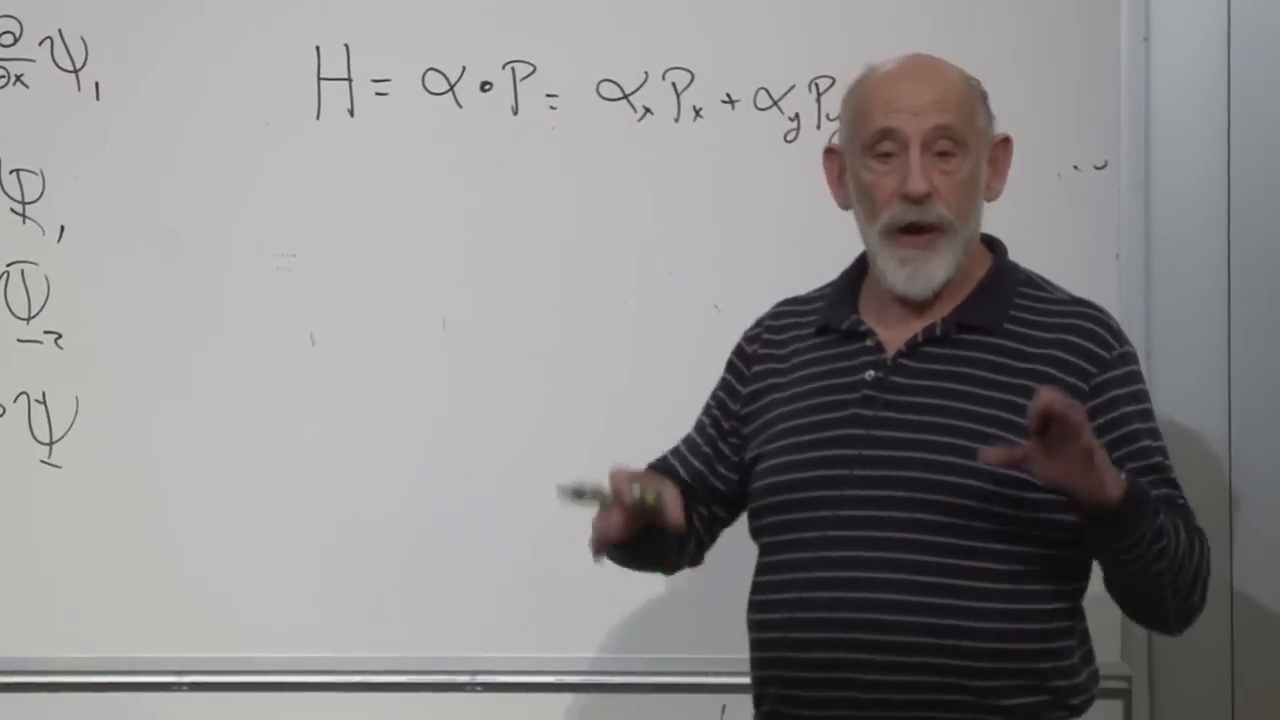
\includegraphics[width=0.94\linewidth]{lecture_10_figure_04.png}
\caption{三維無質量假設\(H=\boldsymbol{\alpha}\cdot\mathbf P\)，圖中正顯示一個矩陣如何成為由三個矩陣組成的向量。}
\lectureframe{00:26:00}
\end{figure}

再次從無質量情形開始。我們要求
\begin{equation}
H^2=\mathbf P^2=P_x^2+P_y^2+P_z^2.
\end{equation}
將式~\eqref{eq:l10-three-d-ansatz}平方後展開，得到
\begin{align}
H^2
&=\alpha_x^2P_x^2+\alpha_y^2P_y^2\\
&\quad+\alpha_z^2P_z^2\\
&\quad+\{\alpha_x,\alpha_y\}P_xP_y\\
&\quad+\{\alpha_x,\alpha_z\}P_xP_z\\
&\quad+\{\alpha_y,\alpha_z\}P_yP_z.
\end{align}
若滿足
\begin{equation}
\alpha_x^2=\alpha_y^2=\alpha_z^2=\mathbb{1},
\end{equation}
對角項就會正確；若滿足
\begin{equation}
\{\alpha_i,\alpha_j\}=0,
\qquad i\ne j.
\label{eq:l10-alpha-anticommutation}
\end{equation}
所有交叉項便會消失。

三個熟知的\(2\times2\)矩陣恰好符合這些要求：
\begin{equation}
\sigma_x=
\begin{pmatrix}
0&1\\
1&0
\end{pmatrix},
\quad
\sigma_y=
\begin{pmatrix}
0&-i\\
i&0
\end{pmatrix},
\quad
\sigma_z=
\begin{pmatrix}
1&0\\
0&-1
\end{pmatrix}.
\label{eq:l10-pauli-matrices}
\end{equation}
因此，一個解為
\begin{equation}
\alpha_i=\sigma_i,
\qquad
H=\boldsymbol{\sigma}\cdot\mathbf P.
\label{eq:l10-weyl-hamiltonian}
\end{equation}

\begin{figure}[htbp]
\centering
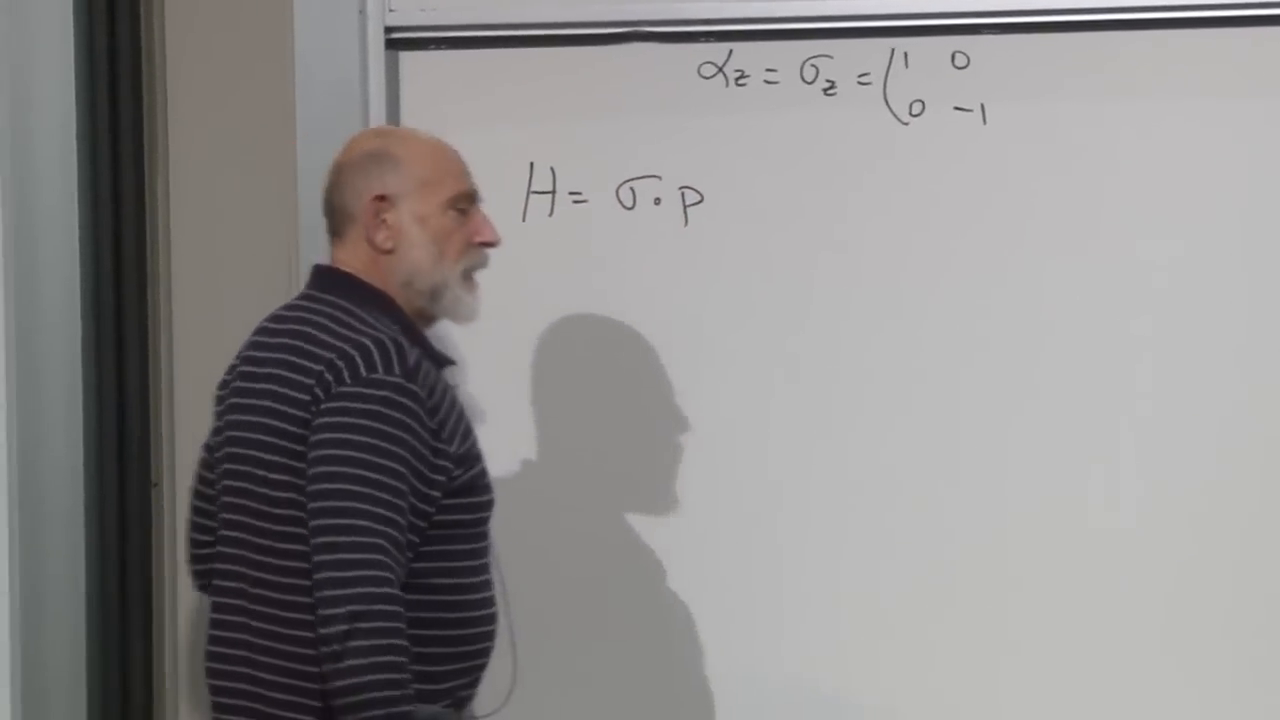
\includegraphics[width=0.94\linewidth]{lecture_10_figure_05.png}
\caption{緊湊的無質量哈密頓量\(H=\boldsymbol{\sigma}\cdot\mathbf P\)；上方仍可看到\(\alpha_z=\sigma_z\)。}
\lectureframe{00:28:16}
\end{figure}

對動量本徵態而言，
\begin{equation}
\boldsymbol{\sigma}\cdot\mathbf p
=
|\mathbf p|\,\boldsymbol{\sigma}\cdot\widehat{\mathbf p}.
\end{equation}
算符\(\boldsymbol{\sigma}\cdot\widehat{\mathbf p}\)的本徵值為\(+1\)和\(-1\)，因此
\begin{equation}
E=\pm|\mathbf p|.
\end{equation}
在這個二分量理論中，正能態的泡利自由度與動量同向，負能態則與動量反向。這種對齊關係是固定的；能量符號給定後，自旋方向不能再獨立調整。

\begin{classroomqa}
\lecturetimestamp{00:30:10}
\audiencequestion{自旋是從狄拉克方程推導出來的，還是因為已知電子具有磁矩，才把自旋放進方程？}
\lecturerresponse{這裡「推導出來」的意思是「作為結果出現」，不是「消失」。我們一開始要求哈密頓量對動量呈線性，且其平方為\(\mathbf P^2\)。普通數無法滿足所需的代數關係，但泡利矩陣可以。因此，線性化本身便帶入了二分量結構。這並不證明每種粒子都必須具有自旋；它表示，以這類狄拉克方程描述的粒子，具有相應的旋量自由度。}
\end{classroomqa}

這是此一構造的核心教訓之一。矩陣不是找到相對論性方程之後才加上的裝飾標記；試圖對相對論性色散關係取局域平方根，便會導出這些矩陣。

\section{為什麼質量需要四個分量}

試著不擴充\(2\times2\)理論，重做一維情形中引入質量的構造：
\begin{equation}
H=\boldsymbol{\sigma}\cdot\mathbf P+\beta m.
\label{eq:l10-failed-mass}
\end{equation}
假設\(\beta^2=\mathbb{1}\)。平方後會出現所需的項\(\mathbf P^2+m^2\)，但也會出現
\begin{equation}
m\sum_i\{\sigma_i,\beta\}P_i.
\end{equation}
若要消去這一項，矩陣\(\beta\)必須滿足
\begin{equation}
\{\sigma_x,\beta\}
=
\{\sigma_y,\beta\}
=
\{\sigma_z,\beta\}
=0.
\label{eq:l10-impossible-beta}
\end{equation}
然而不存在符合要求的\(2\times2\)矩陣。單位矩陣與所有三個泡利矩陣對易，而任何無跡的\(2\times2\)矩陣都是泡利矩陣的線性組合。這類組合都無法與平行於它的分量反對易。\(2\times2\)代數中不存在符合要求的第四個獨立矩陣。

解決方法是擴充旋量。四個彼此反對易且平方為單位矩陣的矩陣，最早可在\(4\times4\)複數表示中實現。選擇這種矩陣大小，不是因為時空有四個維度，而是因為這是能實現所需代數的最小矩陣空間。

等價表示有很多種。對旋量基底作么正變換，會改變所有矩陣的元素，但不會改變任何物理預測。重要的是以下這組抽象關係：
\begin{equation}
\{\alpha_i,\alpha_j\}=2\delta_{ij}\mathbb{1},
\qquad
\{\alpha_i,\beta\}=0,
\qquad
\beta^2=\mathbb{1}.
\label{eq:l10-dirac-algebra}
\end{equation}

\begin{classroomqa}
\lecturetimestamp{00:37:38}
\audiencequestion{能否將\(\beta\)視為時間分量\(\alpha_t\)？}
\lecturerresponse{不能直接這麼看。三個\(\alpha_i\)與\(\beta\)並不會合成單一洛倫茲向量的四個分量。在協變記號中，我們改為定義\(\beta=\gamma^0\)與\(\alpha_i=\gamma^0\gamma^i\)；四個\(\gamma^\mu\)矩陣則滿足時空克利福德代數。}
\end{classroomqa}

一種方便的分塊表示是
\begin{equation}
\alpha_i=
\begin{pmatrix}
\sigma_i&0\\
0&-\sigma_i
\end{pmatrix},
\qquad
\beta=
\begin{pmatrix}
0&I_2\\
I_2&0
\end{pmatrix}.
\label{eq:l10-block-representation}
\end{equation}
對角區塊中的泡利矩陣確保不同的\(\alpha_i\)彼此反對易。\(\beta\)中的非對角單位矩陣區塊則確保\(\beta\)與每個\(\alpha_i\)反對易。

\begin{figure}[htbp]
\centering
\includegraphics[width=0.94\linewidth]{lecture_10_figure_06.png}
\caption{黑板上的\(4\times4\)分塊表示。上方的方程列出所需的反對易關係；完整矩陣則列於式~\eqref{eq:l10-block-representation}。}
\lectureframe{00:41:10}
\end{figure}

有質量的哈密頓量現在為
\begin{equation}
H=\boldsymbol{\alpha}\cdot\mathbf P+\beta m
=
\begin{pmatrix}
\boldsymbol{\sigma}\cdot\mathbf P&mI_2\\
mI_2&-\boldsymbol{\sigma}\cdot\mathbf P
\end{pmatrix}.
\label{eq:l10-massive-dirac}
\end{equation}
利用式~\eqref{eq:l10-dirac-algebra}，可得
\begin{equation}
H^2=\mathbf P^2+m^2.
\end{equation}
因此，四分量結構並非可有可無的修飾；它是在保持方程為一階的同時，容納三維動量與質量項所需的最小結構。

\section{手徵性與額外分量的意義}

擴充旋量後，多出了什麼物理區別？先看無質量的上方區塊，
\begin{equation}
H_R=\boldsymbol{\sigma}\cdot\mathbf P,
\end{equation}
再看無質量的下方區塊，
\begin{equation}
H_L=-\boldsymbol{\sigma}\cdot\mathbf P.
\end{equation}
對正能態而言，第一個區塊的自旋與動量同向，第二個區塊的自旋與動量反向。兩者具有相反的螺旋度。在無質量理論中，螺旋度在正洛倫茲變換下保持不變，因為沒有觀察者能超越類光粒子、反轉其動量，同時維持其自旋方向不變。因此，這兩個區塊描述相反的手徵扇區。

\begin{classroomqa}
\lecturetimestamp{00:41:28}
\audiencequestion{一維情形中，引入質量需要額外的二值自由度。三維情形中，對應的物理區別是什麼？}
\lecturerresponse{是旋量的手徵性。兩個\(2\times2\)區塊中的自旋與動量具有相反的關係：一個是右手性，另一個是左手性。\(4\times4\)理論包含兩者。}
\end{classroomqa}

式~\eqref{eq:l10-massive-dirac}中的質量項是非對角的。它將上方區塊的振幅耦合到下方區塊，反之亦然：
\begin{equation}
\beta m
\begin{pmatrix}
\Psi_R\\
\Psi_L
\end{pmatrix}
=
m
\begin{pmatrix}
\Psi_L\\
\Psi_R
\end{pmatrix}.
\end{equation}
因此，質量會耦合相反手徵性的態。

\begin{classroomqa}
\lecturetimestamp{00:43:58}
\audiencequestion{無質量粒子能改變手徵性嗎？}
\lecturerresponse{在此處顯示的自由無質量哈密頓量中不能。兩個區塊彼此解耦，因此一個起初為右手性或左手性的態會維持原狀。當\(m\ne0\)時，非對角質量項正是混合兩者的原因。}
\end{classroomqa}

對分塊表示而言，這種說法是精確的；但不宜把粒子在兩個箭頭之間機械翻轉的圖像過度延伸。真正的物理敘述，是波動方程中的矩陣耦合。

\begin{classroomqa}
\lecturetimestamp{00:44:50}
\audiencequestion{這些矩陣是由四元數構成的嗎？}
\lecturerresponse{泡利矩陣與四元數單位密切相關：矩陣\(-i\sigma_i\)的平方為\(-\mathbb{1}\)，其乘法也符合四元數的形式，只有方向慣例上的差異。完整的狄拉克矩陣需要更大的克利福德代數，而接下來的論證不需要用到四元數的關聯。}
\end{classroomqa}

\begin{classroomqa}
\lecturetimestamp{00:46:34}
\audiencequestion{若自旋是角動量，這裡是否還有與自旋相關的獨立能量項？}
\lecturerresponse{沒有加入獨立的自由粒子項。旋量結構已透過矩陣納入動能哈密頓量。若將自旋與外加磁場耦合，會引入額外的交互作用項，但那是另一個問題。}
\end{classroomqa}

\section{{\proseunicodefont α}矩陣代表速度，不是自旋}

每個\(\alpha_i\)都有兩個\(+1\)本徵值，也有兩個\(-1\)本徵值。不同分量彼此不對易，因此無法同時精確測量。若要辨明其中一個分量代表什麼，可以使用海森堡方程。對於沒有顯式時間依賴的算符\(L\)，
\begin{equation}
\dot L=i[H,L].
\label{eq:l10-heisenberg}
\end{equation}
此處的符號慣例由Schr\"odinger演化\(e^{-iHt}\)決定。

將式~\eqref{eq:l10-heisenberg}用於位置算符\(x\)。這些矩陣作用於旋量指標，與位置算符對易；只有\(P_x\)不與\(x\)對易：
\begin{align}
\dot x
&=i[\boldsymbol{\alpha}\cdot\mathbf P+\beta m,x]\\
&=i\alpha_x[P_x,x]\\
&=\alpha_x,
\label{eq:l10-velocity}
\end{align}
因為\([P_x,x]=-i\)。因此，\(\alpha_x\)就是速度算符的\(x\)分量；同理，
\begin{equation}
\dot{\mathbf x}=\boldsymbol{\alpha}.
\end{equation}

\begin{classroomqa}
\lecturetimestamp{00:51:50}
\audiencequestion{速度分量的測量結果真的只有\(+1\)或\(-1\)嗎？}
\lecturerresponse{是的。以\(\alpha_i\)為瞬時算符，並採用\(c=1\)單位制時，結果確實如此。一般態不一定是本徵態，因此其期望值可以介於這兩個值之間。有質量粒子的波包平滑傳播，其平均速度低於光速。}
\end{classroomqa}

速度並非守恆量：
\begin{equation}
\dot\alpha_x=i[H,\alpha_x]\ne0.
\end{equation}
含有\(\alpha_y\)、\(\alpha_z\)和\(\beta\)的項都不與\(\alpha_x\)對易。因此，同時含有正能與負能分量的態，其位置會呈現快速振盪的部分。這就是\emph{zitterbewegung}，字面意思是顫動運動。

對遠長於快速振盪週期的時間取平均後，預期的相對論速度為
\begin{equation}
\overline{\mathbf v}=\frac{\mathbf p}{E},
\end{equation}
對低速電子而言，這會化為\(\mathbf p/m\)。

\begin{classroomqa}
\lecturetimestamp{00:54:40}
\audiencequestion{自由電子沒有外力卻在顫動，是否違反牛頓定律？}
\lecturerresponse{不會。平移不變性保證動量守恆，因此\(\dot{\mathbf P}=0\)。狄拉克速度算符並不等同於\(\mathbf P/m\)；即使動量保持不變，其快速振盪部分仍可改變。時間平均後的運動符合預期的自由粒子關係。}
\end{classroomqa}

\begin{classroomqa}
\lecturetimestamp{00:55:22}
\audiencequestion{速度總是\(c\)嗎？}
\lecturerresponse{對單一\(\alpha_i\)作瞬時測量，其本徵值為\(\pm c\)；但有質量的波包通常是疊加態，其期望值低於光速。其平均群速度為\(\mathbf p/E\)。}
\end{classroomqa}

\begin{classroomqa}
\lecturetimestamp{00:55:30}
\audiencequestion{可以把這種振盪想成質量使速度改變嗎？}
\lecturerresponse{不可以。質量是固定參數。這種振盪來自速度算符與哈密頓量算符彼此不對易；等價地說，它來自不同能量扇區之間的干涉，而不是質量有所波動。}
\end{classroomqa}

\begin{classroomqa}
\lecturetimestamp{00:56:22}
\audiencequestion{瞬時測量能否發現速度指向一個方向，但平均運動卻指向另一個方向？}
\lecturerresponse{可以。分量算符的本徵值是兩個確定值，而重複測量或時間平均測量會呈現較平滑的漂移。}
\end{classroomqa}

「自旋」一詞也必須謹慎使用。\(\alpha_i\)的分量依照速度這種普通向量的方式變換。在此表示中，真正的自旋算符是
\begin{equation}
\mathbf S=\frac12\boldsymbol{\Sigma},
\qquad
\Sigma_i=
\begin{pmatrix}
\sigma_i&0\\
0&\sigma_i
\end{pmatrix}.
\label{eq:l10-spin-operator}
\end{equation}
它與\(\alpha_i\)的差異在於下方區塊的符號相反。兩者的矩陣密切相關，但速度與自旋並非同一個可觀測量。

\section{負能量與最低能量真空}

在引入這些矩陣工具之前，負能量問題就已經存在。回到一維的右行解，
\begin{equation}
H=P.
\end{equation}
由於\(p\)涵蓋整條實數軸，\(E=p\)便沒有下界。

真空不能只定義為沒有粒子的態；它必須是無法再從中取出能量的態。若在空態中加入一個負能量粒子就能降低能量，而後還能再加入一個並無限延續下去，那麼這個空態就不是穩定的真空。

費米統計提供了一種歷史上的解法：在每個負能態中放入一個電子。每加入一個電子，總能量都會降低；但排他原理限制每個單粒子態只能有一個電子。所有負能態填滿後，便沒有其他電子能再落入這些態。狄拉克將這種填滿的組態視為真空。

同樣的構造若用於玻色子，就會失效。任意多個玻色子都能佔據同一個態，因此負能玻色子模態可以不受限制地吸收粒子。講座一開始介紹的費米子佔據數限制\(n=0,1\)，正是阻止能量不斷下降的關鍵。

\begin{figure}[htbp]
\centering
\includegraphics[width=0.94\linewidth]{lecture_10_figure_07.png}
\caption{黑板上的歷史性狄拉克海圖像：負能級一路填滿至分界線，正能態則位於其上方。}
\lectureframe{01:02:45}
\end{figure}

\begin{figure}[htbp]
\centering
\begin{adjustbox}{max width=\linewidth}
\begin{tikzpicture}[x=1.05cm,y=0.72cm,>=Latex]
\draw[->] (0,-4.8) -- (0,4.8) node[above] {$E$};
\draw[thick] (-2.9,0) -- (3.2,0) node[right] {$E=0$};
\foreach \y in {-4,-3.3,...,-0.5} {
  \draw (-2.3,\y) -- (2.3,\y);
  \foreach \x in {-1.8,-1.2,...,1.8} {
    \fill[blue!65!black] (\x,\y) circle (1.6pt);
  }
}
\foreach \y in {0.8,1.6,...,4.0} {
  \draw (-2.3,\y) -- (2.3,\y);
}
\draw[red,very thick] (0.6,-2.6) circle (5pt);
\draw[red,->,very thick] (0.6,-2.35) .. controls (1.4,-0.4) and (1.2,1.6) .. (1.5,2.4);
\fill[red] (1.5,2.4) circle (2.5pt);
\node[right,red] at (0.85,-2.6) {hole};
\node[right,red] at (1.7,2.4) {$e^-$};
\node[left] at (-2.5,-2.2) {filled negative-energy states};
\end{tikzpicture}
\end{adjustbox}
\caption{填滿的狄拉克海之上的激發：將一個負能量電子提升後，留下正能量空穴。}
\end{figure}

狄拉克海是對正確算符重排的一種歷史性描述。不能把它字面上的無限電荷與能量，誤認為可直接觀測的物理量；現代重新表述後，便不必再想像有實際電子填滿整個空間。

\section{空穴就是正電子}

所有負能態都被佔據後，可能出現兩種激發：我們可以在海之上加入一個正能量電子；也可以移除一個負能量電子，留下空穴。

空穴帶有與缺失電子相反的電荷。移除電荷\(-e\)，會使電荷改變\(+e\)。空穴也具有正的激發能。若被移除電子的能量為\(E_-<0\)，相對於填滿的真空，能量變化為
\begin{equation}
E_{\mathrm{hole}}=-E_->0.
\end{equation}
空穴是帶正電的正能量激發，也就是正電子。

光子可以將狄拉克海中的電子提升到正能態。相對於真空，末態包含一個電子和一個正電子。在時間排序圖中，慣例上將電子的電子數流向畫成向上，而正電子線則畫上相反方向的箭頭。這些箭頭表示費米子數或電荷的流向，並非微小的經典速度向量。

\begin{classroomqa}
\lecturetimestamp{01:05:14}
\audiencequestion{這種圖像是否要求電子和正電子數量相等？}
\lecturerresponse{不要求任意態都如此。從真空出發產生一對中性粒子時，會各有一個電子和正電子；但某個態原本就可能含有較多電子或較多正電子。電荷守恆會限制反應，卻不要求所有允許的態都具有相等的粒子數。}
\end{classroomqa}

狄拉克最初並不知道這個空穴會是質量與電子相同、只有電荷及其他可加量子數相反的粒子。正電子尚未納入熟知的粒子清單前，狄拉克方程和空穴構造便已導出這項預測。

\section{一個費米子場同時包含電子與正電子}

場算符將歷史圖像轉化為現代代數。暫且略去旋量指標、歸一化因子與時間依賴。一維場可以示意性地展開為
\begin{equation}
\psi(x)
\sim
\int_{-\infty}^{\infty}dp\,a(p)e^{ipx}.
\label{eq:l10-full-field-integral}
\end{equation}
對右行色散關係\(E=p\)而言，正的\(p\)標記正能量，負的\(p\)則標記負能量。將積分拆開：
\begin{equation}
\psi(x)
\sim
\int_0^\infty dp\,a(p)e^{ipx}
+
\int_{-\infty}^0 dp\,a(p)e^{ipx}.
\end{equation}
在第二項中令\(p=-q\)，其中\(q>0\)，並將湮滅一個已佔據負能態的電子，重新詮釋為產生一個正電子：
\begin{equation}
b^\dagger(q):=a(-q).
\end{equation}
於是
\begin{equation}
\psi(x)
\sim
\int_0^\infty dp\,
\left[
a(p)e^{ipx}
+
b^\dagger(p)e^{-ipx}
\right].
\label{eq:l10-electron-positron-split}
\end{equation}
平面波相位的確切符號取決於時空慣例；不受慣例影響的內容是，\(\psi\)包含電子湮滅算符與正電子產生算符。

\begin{figure}[htbp]
\centering
\includegraphics[width=0.94\linewidth]{lecture_10_figure_08.png}
\caption{將場積分拆分為正能量與負能量兩個部分。下方一行將負能量電子算符重新標記為正電子產生算符。}
\lectureframe{01:11:35}
\end{figure}

這正是式~\eqref{eq:l10-fermion-mode}所呈現的滿態與空態對稱性派上用場之處。對費米子而言，算符代數允許這種重新標記，同時保留反對易結構。

示意性的電磁交互作用可寫成
\begin{equation}
H_{\mathrm{int}}
\sim
\int dx\,\psi^\dagger(x)\psi(x)A(x),
\label{eq:l10-qed-schematic}
\end{equation}
其中\(A\)表示光子場。由於每個費米子場都包含電子與正電子部分，一個局域算符便涵蓋了數種反應通道：
\begin{align}
e^-&\longrightarrow e^-+\gamma,\\
e^-+e^+&\longrightarrow\gamma,\\
\gamma&\longrightarrow e^-+e^+,
\end{align}
此外還有這些過程的反向與交叉過程。能量—動量守恆決定特定環境下哪些通道在運動學上可行。例如，真空中的孤立實光子無法產生電子—正電子對，除非有另一個參與者吸收反衝；即使如此，相互作用中仍存在這個局域頂點。

\begin{figure}[htbp]
\centering
\includegraphics[width=0.94\linewidth]{lecture_10_figure_09.png}
\caption{黑板並列了電子放射、電子—正電子對湮滅，以及示意性交互作用\(\psi^\dagger\psi A\)。從相同場算符中選取不同部分，就會得到不同反應通道。}
\lectureframe{01:13:30}
\end{figure}

因此，單一簡潔的場算符乘積便統整了許多表面上不同的反應。費曼後來提出了系統化的圖解規則，用來計算振幅；不過，這裡已經顯示出大部分算符結構。

\section{現代真空概念與費米海類比}

\begin{classroomqa}
\lecturetimestamp{01:14:20}
\audiencequestion{現代物理學家如何描述這件事，而不把真空視為字面上的狄拉克海？}
\lecturerresponse{他們直接重新詮釋算符：將負能量電子的湮滅重新命名為正能量正電子的產生，並將真空定義為會被所有電子與正電子湮滅算符消去的態。這樣得到的表述對稱地處理粒子與反粒子，也不需要假設有實質的粒子海。}
\end{classroomqa}

歷史上的海仍有參考價值，因為它的邏輯與凝聚態物質中的情形十分相似。在晶體中，固定數量的電子會填滿最低的可用單粒子態，直到費米能階。填滿的基態並非空無一物。若將一個電子激發到費米能階以上，就會在其下方留下一個未佔據態。相對於填滿的背景，這個空穴具有正的激發能，並可表現為帶正電的載子。

兩者仍有重要差異。固體中的空穴存在於介質中，其有效質量和電荷響應取決於能帶結構。正電子則是相對論量子場中的基本反粒子。即使如此，共通的粒子—空穴代數仍使這個類比很有力。

\begin{classroomqa}
\lecturetimestamp{01:17:14}
\audiencequestion{玻色子的克萊因--戈登理論也會同樣地級聯到負能量態嗎？}
\lecturerresponse{不會。經過適當量子化的複數克萊因--戈登場，會以正能量粒子和反粒子的形式加以組織，而不需要填滿玻色子海。它的二階方程和正則結構不同於狄拉克哈密頓量的建構方式，因此不能將歷史上的費米子海論證原封不動地套用過來。}
\end{classroomqa}

\begin{classroomqa}
\lecturetimestamp{01:17:30}
\audiencequestion{玻色子的自旋為一是從何而來？}
\lecturerresponse{不是來自這裡使用的泡利矩陣線性化。自旋為一的場有各自的洛倫茲變換律和場方程。這裡的推導說明的是狄拉克費米子的旋量結構，並不涵蓋所有可能的粒子自旋。}
\end{classroomqa}

\begin{classroomqa}
\lecturetimestamp{01:17:46}
\audiencequestion{為什麼負能量解必須遵循費米統計？}
\lecturerresponse{因為泡利不相容原理限制每個態至多容納一個電子。一旦所有負能量態都已佔據，就沒有電子能再落入其中。玻色子的佔據數沒有這種上限，因此若照字面構想負能量玻色子海，它仍然沒有底。}
\end{classroomqa}

\begin{classroomqa}
\lecturetimestamp{01:20:02}
\audiencequestion{電子與正電子的區別，是否只是另一種二元自由度，就像電荷一樣？}
\lecturerresponse{就態的計數而言，有質量的狄拉克場有兩種電子自旋態和兩種正電子自旋態，因此用兩個二元標籤來記憶很有幫助。但粒子與反粒子的區別，並不是單一電子中可獨立旋轉的內部量子位元：每個電子的電荷都是\(-e\)，每個正電子的電荷都是\(+e\)；量子化之後，這項區別才從正、負頻部分中顯現出來。}
\end{classroomqa}

無限大的海引出最後一個問題。

\begin{classroomqa}
\lecturetimestamp{01:20:54}
\audiencequestion{無限大的狄拉克海會產生無限大的宇宙常數嗎？}
\lecturerresponse{這凸顯了真空能問題。玻色子零點模貢獻\(+\tfrac12\hbar\omega\)，而費米子模的貢獻符號相反。若兩者的譜相符，形式上可能相消；但電子譜與光子譜並不相符，因此預期會留下極大的剩餘量。沒有重力時，可以扣除哈密頓量中的常數項，因為只有能量差有意義。有重力時，絕對真空能會產生引力效應，因此扣除這一項便成了物理問題，而不只是記帳方式。}
\end{classroomqa}

最後要回到質量的意義。

\begin{classroomqa}
\lecturetimestamp{01:22:56}
\audiencequestion{我們能進一步說明質量如何關聯左手與右手分量嗎？}
\lecturerresponse{精確的說法已經寫在哈密頓量中：非對角項\(m\beta\)將一個手徵區塊映射到另一個區塊。若要用更具體、機械式的圖像描述微觀翻轉，也可以這麼做，但那種圖像終究不完整。}
\end{classroomqa}

\end{document}
